%% 采析绘使用手册（MiKTeX / xelatex 编译两趟；PDF 是构建产物，不进仓库）
%% 本文件就是全书的版式模板（ch02…ch10 只写正文，不设版式）。全文仿宋，正文五号，页面上下 2.54cm 左右 3.18cm，
%% 一级标题三号加粗、二级标题五号加粗，均不编号、左对齐，图题写 图N，表题写 表N。
\documentclass[a4paper]{article}
\usepackage[UTF8]{ctex}
\usepackage{fontspec}
\usepackage{graphicx}
\usepackage{booktabs}
\usepackage{tabularx}
\usepackage{multirow}
\usepackage{array}
\usepackage[table]{xcolor}
\usepackage{caption}
\usepackage{float}
\usepackage{enumitem}
\usepackage{amsmath}
\usepackage{tikz}
\usetikzlibrary{arrows.meta,positioning,calc,shapes.geometric,backgrounds,fit}
\usepackage{pgfplots}
\pgfplotsset{compat=1.18}
\usepackage[left=3.18cm,right=3.18cm,top=2.54cm,bottom=2.54cm,headheight=0pt,headsep=0pt,footskip=1.2cm]{geometry}
\usepackage{titlesec}
\usepackage[hidelinks,bookmarks=true]{hyperref}
\usepackage{tocloft}
\renewcommand{\cftsecfont}{\bfseries}
\renewcommand{\cftsecpagefont}{\bfseries}
\renewcommand{\cftsecleader}{\cftdotfill{\cftdotsep}}
\setlength{\cftbeforesecskip}{7pt}
\setlength{\cftbeforesubsecskip}{2pt}
\renewcommand{\cftsubsecfont}{\normalsize}

\setCJKmainfont{FangSong}[AutoFakeBold=2.0]
\setCJKsansfont{FangSong}[AutoFakeBold=2.0]
\setCJKmonofont{FangSong}[AutoFakeBold=2.0]
\setmainfont{FangSong}[AutoFakeBold=2.0]
\setsansfont{FangSong}[AutoFakeBold=2.0]
% 代码与路径用真正的等宽字体，与中文正文分开
\IfFontExistsTF{Consolas}
  {\setmonofont{Consolas}[Scale=0.92]}
  {\IfFontExistsTF{DejaVu Sans Mono}
    {\setmonofont{DejaVu Sans Mono}[Scale=0.9]}
    {\setmonofont{Latin Modern Mono}}}

\setcounter{secnumdepth}{-1}
\setcounter{tocdepth}{1}
\titleformat{\section}[block]{\normalfont\bfseries\fontsize{16}{22}\selectfont}{}{0pt}{}
\titlespacing*{\section}{0pt}{24pt}{20pt}
\titleformat{\subsection}[block]{\normalfont\bfseries\fontsize{10.5}{15}\selectfont}{}{0pt}{}
\titlespacing*{\subsection}{0pt}{18pt}{14pt}
\titleformat{\subsubsection}[runin]{\normalfont\bfseries\fontsize{10.5}{15}\selectfont}{}{0pt}{}

\captionsetup{font=normalsize,labelfont=bf,labelsep=quad,skip=6pt}
\captionsetup[figure]{name=图}
\captionsetup[table]{name=表}
\renewcommand{\arraystretch}{1.22}
\setlist[enumerate]{leftmargin=1.6em,itemsep=3pt,topsep=3pt,parsep=0pt}
\setlist[itemize]{leftmargin=1.4em,itemsep=3pt,topsep=3pt,parsep=0pt,label=\ensuremath{\bullet}}
\graphicspath{{./img/}}

% ─── 采析绘配色，取前端的设计令牌 ───
\definecolor{cA}{HTML}{22557A}   % 图表首色，深板岩蓝
\definecolor{cB}{HTML}{B5563C}
\definecolor{cC}{HTML}{3E7A5A}
\definecolor{cD}{HTML}{C79A3B}
\definecolor{cE}{HTML}{6A5A8C}
\definecolor{cF}{HTML}{2E7D8C}
\definecolor{ink}{HTML}{1A1A1A}
\definecolor{paper}{HTML}{FFFFFF}
\definecolor{grid}{HTML}{EDEBE6}
\definecolor{okc}{HTML}{4E8061}
\definecolor{warnc}{HTML}{9A7740}
\definecolor{errc}{HTML}{A85454}
\definecolor{src}{HTML}{4A6FA5}
\definecolor{upc}{HTML}{4A8FA5}
\definecolor{prc}{HTML}{A85454}
\definecolor{anl}{HTML}{9A7740}
\definecolor{bib}{HTML}{3D7A72}
\definecolor{viz}{HTML}{4E8061}
\definecolor{cmt}{HTML}{B0567A}
\definecolor{outc}{HTML}{6F7F8A}
\definecolor{namec}{HTML}{3A4A5A}

% ─── 全书共用的插图样式，对齐前端的 OMM-ZEN 视觉 ───
% 纸白底、墨色细线、极小圆角、左侧一道类型色条、灰阶层次而不是重色块。
\tikzset{
  card/.style={draw=ink!15,line width=0.4pt,rounded corners=2pt,fill=paper,
    align=center,font=\small,inner sep=6pt,minimum height=1.0cm,
    path picture={\fill[#1] ([xshift=2.2pt]path picture bounding box.north west)
      rectangle ([xshift=3.6pt]path picture bounding box.south west);}},
  card/.default=cA,
  chip/.style={draw=ink!13,line width=0.4pt,rounded corners=2pt,fill=paper,
    align=center,font=\scriptsize,inner sep=4pt},
  ghost/.style={draw=none,fill=none,align=center,font=\scriptsize,inner sep=2pt},
  wire/.style={-{Latex[length=1.8mm,width=1.3mm]},draw=ink!28,line width=0.5pt},
  softwire/.style={draw=ink!16,line width=0.45pt},
  tag/.style={font=\scriptsize,text=ink!45,inner sep=1pt},
  micro/.style={font=\tiny,text=ink!35,inner sep=1pt},
  badge/.style={circle,draw=ink!18,line width=0.4pt,fill=paper,
    text=ink!50,font=\scriptsize,inner sep=1.4pt},
  rule/.style={draw=ink!15,line width=0.4pt},
  accentline/.style={draw=#1,line width=1.6pt},
  accentline/.default=cA
}
\arrayrulecolor{ink!30}
\setlength{\aboverulesep}{0.35ex}
\setlength{\belowrulesep}{0.35ex}

% 小注一行，用在插图里的次要说明
\newcommand{\micro}{\fontsize{7}{9}\selectfont\color{ink!45}}

\begin{document}
\fontsize{10.5}{13.1}\selectfont

\thispagestyle{empty}

\begin{center}
\vspace*{2.2cm}
{\bfseries\fontsize{26}{34}\selectfont 采析绘使用手册\par}
\vspace{10pt}
{\bfseries\fontsize{13}{20}\selectfont 从采集到论文图的一条流水线\par}
\vspace{26pt}

\begin{tikzpicture}[scale=0.98]
  \node[card=cA,minimum width=2.6cm] (a) at (0,0) {采集\\[2pt]\micro 十个平台};
  \node[card=cC,minimum width=2.6cm] (b) at (3.5,0) {清洗\\[2pt]\micro 去重与筛选};
  \node[card=anl,minimum width=2.6cm] (c) at (7.0,0) {分析\\[2pt]\micro 模型与主题};
  \node[card=viz,minimum width=2.6cm] (d) at (10.5,0) {成图\\[2pt]\micro 论文样式};
  \draw[wire] (a) -- (b);
  \draw[wire] (b) -- (c);
  \draw[wire] (c) -- (d);
  \node[micro,below=9pt of b] {数据一行行落下};
  \node[micro,below=9pt of c] {每一步都能重来};
\end{tikzpicture}

\vspace{30pt}
{\fontsize{11}{18}\selectfont 所有截图都来自真实运行，例子都是仓库里带着的工作流\par}
\end{center}

\vfill
\begin{center}
{\fontsize{9}{14}\selectfont 版本对应仓库 main 分支，二〇二六年十一月\par}
\end{center}

\newpage

\tableofcontents

\newpage

\section{它做什么}

一句话，它把网页上的公开内容变成一张能分析的表格，再把表格变成论文里的图。

中间那一步是重点。它不替你写论文，也不替你选题目，它负责把重复的体力活接成流水线。
一条流水线上有若干节点，节点之间用线连着，数据从左往右流。你按下执行，程序按顺序把每个节点跑一遍，
每一步的中间结果都存进本地数据库，所以断网、关机、中途停下都不至于从头再来。

\begin{figure}[H]\centering
\begin{tikzpicture}[node distance=5mm,scale=0.92,transform shape]
  \node[card=cA,text width=2.9cm] (src) {采集\\[2pt]\micro 浏览器抓公开页面};
  \node[card=cC,right=of src,text width=2.9cm] (clean) {整理\\[2pt]\micro 清洗与去重};
  \node[card=anl,right=of clean,text width=2.9cm] (ana) {理解\\[2pt]\micro 模型读文本};
  \node[card=viz,right=of ana,text width=2.9cm] (viz) {表达\\[2pt]\micro 图与表};

  \node[chip,below=7mm of src,text width=2.9cm] (login) {登录状态\\ Cookie 与 profile};
  \node[chip,below=7mm of clean,text width=2.9cm] (dedupe) {三层去重\\ 精确、归一、近重复};
  \node[chip,below=7mm of ana,text width=2.9cm] (model) {本地 Ollama\\ 或 OpenRouter};
  \node[chip,below=7mm of viz,text width=2.9cm] (tex) {PNG、SVG\\ LaTeX 与 PDF};

  \draw[softwire] (login) -- (src);
  \draw[softwire] (dedupe) -- (clean);
  \draw[softwire] (model) -- (ana);
  \draw[softwire] (tex) -- (viz);

  \begin{scope}[on background layer]
    \node[draw=ink!10,line width=0.4pt,dashed,rounded corners=3pt,fit=(src)(viz)(login)(tex),inner sep=7pt] (all) {};
  \end{scope}
  \node[micro,above=2pt of all] {一条工作流，四段分工，任何一段都能单独重跑};
\end{tikzpicture}
\caption{采析绘的四段分工}
\end{figure}

谁在干活，分三种角色。人负责选题、填参数、看图；程序负责翻页、等待、写库、算数；模型只负责读文字，
判断这段话是夸还是骂、这一簇文章在谈什么。三者边界清楚，所以模型没启动时，除了模型那一步，别的照常能跑。

它适合的活有一类共同点：材料是文字，量在几千到几万条，来源在公开网页或文献库里，最后要出成图表或者论文。
课程作业、毕业论文、课题报告，基本都是这个形状。

按钮名和字段名在书里用等宽字体，比如 \texttt{执行}、\texttt{目标数量}。凡是我说它拒绝的，
意思都是它会在开始前停下并写清原因，不会闷头跑完再给你一张空表。

\section{云端试用}

不想先折腾环境，可以直接用浏览器打开云端已部署的一份。

\begin{center}
\begin{minipage}{0.92\textwidth}
\rule{\linewidth}{0.4pt}\\[5pt]
{\bfseries 云端入口}\quad{\fontsize{11}{16}\selectfont\texttt{http://47.116.114.77/crawler}}\\[5pt]
只要能上网就能打开，不用装 Python，不用配 Chrome，也不用在本机跑模型。
工作流、数据集、运行记录都在服务器上，换一台电脑登录同一个账号，东西还在。\\[3pt]
账号由站点管理员开通。登录以后可以新建画布、上传表格、接分析节点、出图，与本地版是同一套界面。\\[3pt]
云端为了安全和速度，关掉了本地模型的界面，采集一律在后台跑，也不允许在服务器上弹出浏览器扫码登录。
红果短剧那种要在本机播放器上旁听的采集只能在 Windows 本地做；其余靠公开页面就能读的部分，云端都能跑。\\[4pt]
\rule{\linewidth}{0.4pt}
\end{minipage}
\end{center}

云端与本地共用同一套操作。要真的采数据、跑本地模型、编 PDF 时，再回本机按下一节装好环境。

\section{安装}

要装的东西分四层，缺哪层它就在控制台点名说缺哪层。

\begin{enumerate}
\item Python 3.11 以上。代码里用了 \texttt{zip(strict=True)} 这类新语法，系统自带的 3.9 会直接报错。
\item Chrome 浏览器，外加一个和它大版本一致的 chromedriver。程序不会替你联网下载驱动，这一点是有意的。
\item 本地大模型用 Ollama，或者在设置里填一个 OpenRouter 的 Key。两个都不配也能跑，只是模型相关的节点用不了。
\item 要出 PDF 图和论文成稿，再装一个 TeX 发行版。Windows 上装 MiKTeX，装的时候把中文支持勾上。
\end{enumerate}

先在项目根目录建虚拟环境，在虚拟环境里装依赖。

\begin{quote}\small
\texttt{python -m venv .venv}\\
\texttt{.venv\textbackslash Scripts\textbackslash activate}（Linux 与 macOS 用 \texttt{source .venv/bin/activate}）\\
\texttt{pip install -r requirements.txt}\\
\texttt{ollama pull qwen3.5:9b}（用 OpenRouter 可以跳过）
\end{quote}

启动时一定要进入 \texttt{backend} 目录，那里是导入的根，从别处启动会找不到模块。

\begin{quote}\small
\texttt{cd backend}\\
\texttt{python app.py}
\end{quote}

浏览器打开 \texttt{127.0.0.1:5000} 就是界面。端口和监听地址可以用环境变量 \texttt{PORT} 与 \texttt{HOST} 改。
程序默认只监听本机，也不会自己弹浏览器，这两条都是安全的默认值。

第一次启动会在项目根目录建出 \texttt{data/} 与 \texttt{logs/}。运行记录、数据集、登录状态、导出文件都在 \texttt{data/} 里，
只有 \texttt{data/workflows/} 跟着仓库走。换电脑时把整个 \texttt{data/} 一起搬，工作流才找得到它引用的数据集。

同一份数据目录同时只能开一个服务。两个实例会互相当成对方中断，把正在写的运行标成异常。要同时开第二个，
给其中一个指定自己的数据根，两边互不干涉。程序只在 \texttt{backend/} 里跑，从别处启动会找不到模块。

\section{第一次打开}

页面打开后先看三处：左上角节点库，中间带网格的画布，底部一排面板按钮与状态栏。

\begin{enumerate}
\item 在节点库搜索框里输入 \texttt{数据源}，列表只剩匹配项。
\item 点 \texttt{数据源} 一次，画布中央落下一个节点。
\item 点右上角“\texttt{样式}”，主题选“\texttt{深色}”，界面与图表配色一起变暗；再选回“\texttt{浅色}”。
\item 删掉刚才那个节点：选中后按 Delete。
\end{enumerate}

底部若出现一行红字，先读它。常见的是模型服务连不上、数据目录被占用、浏览器驱动找不到。这些都不阻止界面打开，
只影响用到那项能力的节点。

界面有中英两套文案，右上角的“\texttt{中文}”与“\texttt{EN}”随时切。切换只影响显示，不改数据，也不会让已保存的工作流失效。

\section{界面}

界面是一整块，从上到下五条带，从左到右三列。

\begin{enumerate}
\item 菜单条。文件、编辑、视图、样式、运行、数据、语言都在这一行，平铺不藏二级菜单。
\item 节点库。按工作流、数据输入、数据处理、结果输出四组排列，点一下把节点放到画布中央，也可以按住拖到指定位置。
\item 画布。网格底，节点在这里摆放与连线，滚轮缩放，空白处拖动平移，左下角有缩略图。
\item 大纲。当前画布的节点清单，点一条就把镜头移过去，节点多的时候靠它找路。
\item 停靠面板。控制台、进程监控、运行记录、定时任务、文献计量、导出产物、已保存的登录、数据集、词库、工作流文件都在这里，点底部的按钮打开，一次只开一个，再点一次收起。
\item 状态栏。节点数、预计行数、预计调用模型次数、缩放比例，运行前扫一眼能省不少等待。
\end{enumerate}

\begin{figure}[H]\centering
\begin{tikzpicture}
\node[anchor=south west,inner sep=0] (shot) at (0,0) {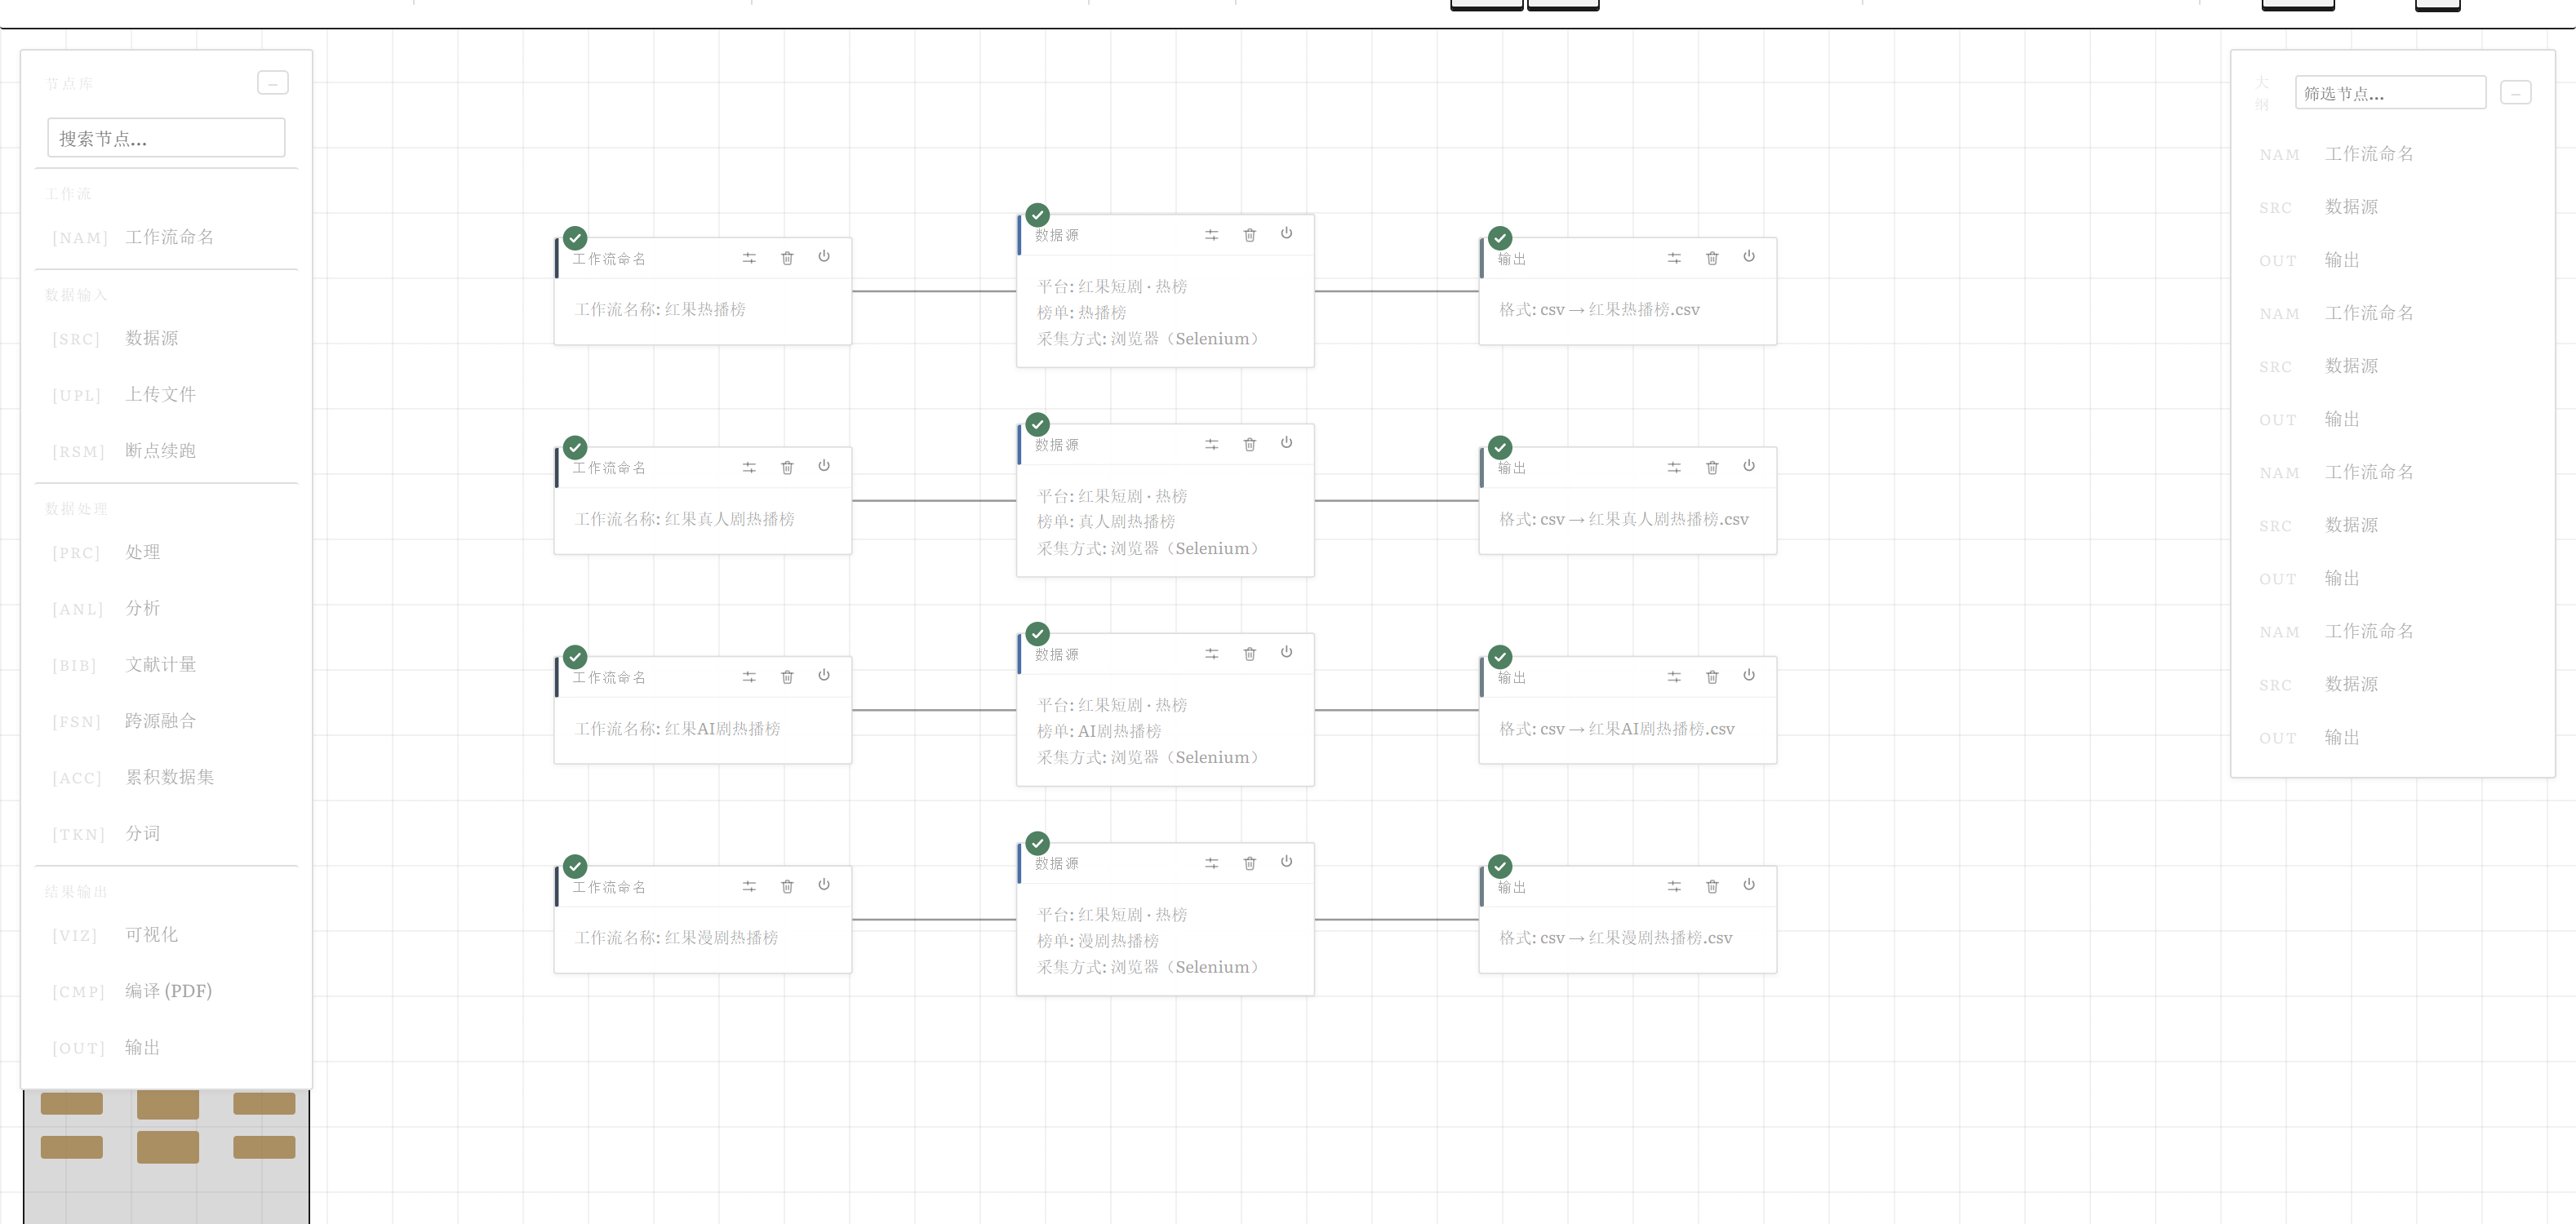
\includegraphics[width=\textwidth]{hg-canvas.png}};
\node[badge,fill=paper] at ([xshift=0.45cm,yshift=-0.40cm]shot.north west) {1};
\node[badge,fill=paper] at ([xshift=0.55cm,yshift=-2.35cm]shot.north west) {2};
\node[badge,fill=paper] at ([xshift=6.9cm,yshift=-2.55cm]shot.north west) {3};
\node[badge,fill=paper] at ([xshift=-1.0cm,yshift=-1.55cm]shot.north east) {4};
\node[badge,fill=paper] at ([xshift=1.05cm,yshift=0.65cm]shot.south west) {5};
\node[badge,fill=paper] at ([xshift=-0.75cm,yshift=0.25cm]shot.south east) {6};
\end{tikzpicture}
\caption{界面的六块区域，画布里是一份跑过的红果工作流}
\label{fig:ui-map}
\end{figure}

\subsection{大纲}

大纲按画布顺序列出每个节点，左边是类型代码，右边是标题。顶部搜索框按标题筛选，点一条就把画布镜头对准它并选中。
面板右上角的减号把大纲折成一条窄边，给画布让出宽度。

\begin{figure}[H]\centering
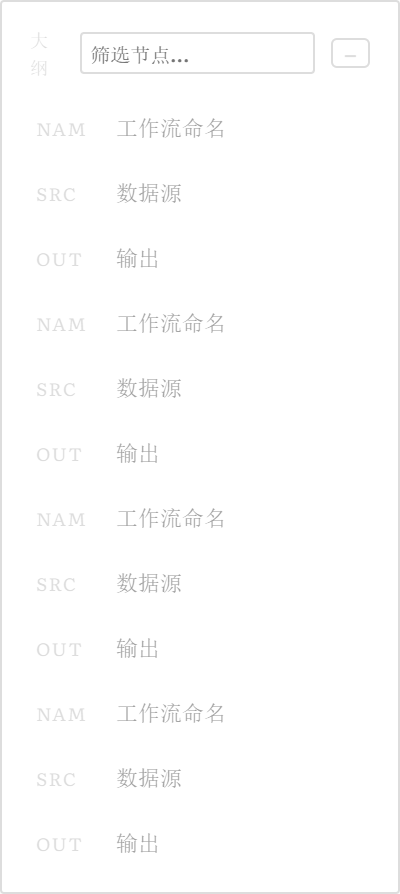
\includegraphics[width=0.43\textwidth]{outline.png}
\caption{大纲：搜索、类型代码、标题，点一条跳过去}
\label{fig:outline}
\end{figure}

\subsection{停靠面板}

底部一行按钮各管一个面板。面板从底部升起，占屏幕下半部分，再点同一个按钮收起。每个面板的内容都是服务端现算的，
所以看到的是这一刻的真实状态，不是页面打开时的旧快照。

\begin{table}[H]\centering
\caption{停靠面板一览}
\label{tab:docks}
\small
\begin{tabularx}{\textwidth}{p{2.6cm}X}
\toprule
面板 & 内容 \\
\midrule
控制台 & 本轮运行的实时日志，按工作流分页签，可按级别过滤、搜索、下载 \\
进程监控 & 服务内正在跑的后台线程，看得出哪个采集卡住了 \\
运行记录 & 每次运行的状态、节点数、行数、耗时，能载入某次结果、看日志、出报告、删除 \\
定时任务 & 按天、按周、按间隔或 cron 定时执行一张已存画布 \\
文献计量 & 已建网项目的快照与跨运行对比 \\
导出产物 & 所有落盘文件，下载、删除、复制路径 \\
已保存的登录 & 每个平台每个账号的 Cookie 与浏览器目录 \\
数据集 & 上传过的表格，来源、列数、行数、被谁引用 \\
词库 & 停用词与领域词 \\
工作流文件 & 打开、重命名、导入导出、打包成项目 \\
\bottomrule
\end{tabularx}
\end{table}

\begin{figure}[H]\centering
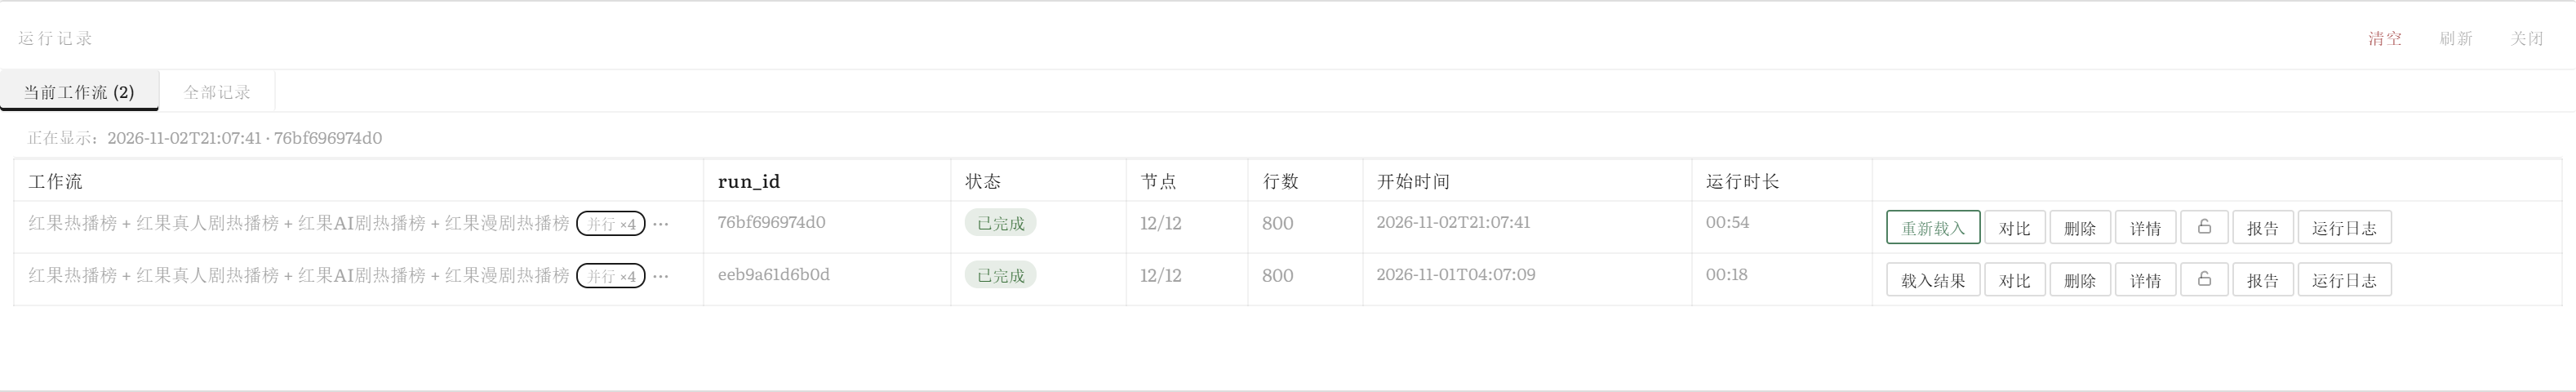
\includegraphics[width=0.98\textwidth]{runs-panel.png}
\caption{运行记录：状态、节点数、行数、耗时与每一行的操作}
\label{fig:runs-panel}
\end{figure}

\begin{figure}[H]\centering

\includegraphics[width=0.43\textwidth]{datasets.png}
\caption{数据集面板，一份表格一行}
\label{fig:datasets}
\end{figure}

\subsection{样式}

菜单条的“\texttt{样式}”管三件事：背景、主题、排布，另加一个圆角滑杆。背景有五档由浅到深的底纹，
主题有自动、浅色、深色三档，自动跟随系统。排布选“\texttt{算法排布}”按连线分层摆放，
选“\texttt{布局基准}”恢复你为这份工作流存过的位置；基准要先保存工作流才能选。
“\texttt{打开画布历史}”给当前状态起名存档，一次最多一百份，恢复之前列出与当前状态的差异，恢复本身也算一步撤销。

\begin{figure}[H]\centering
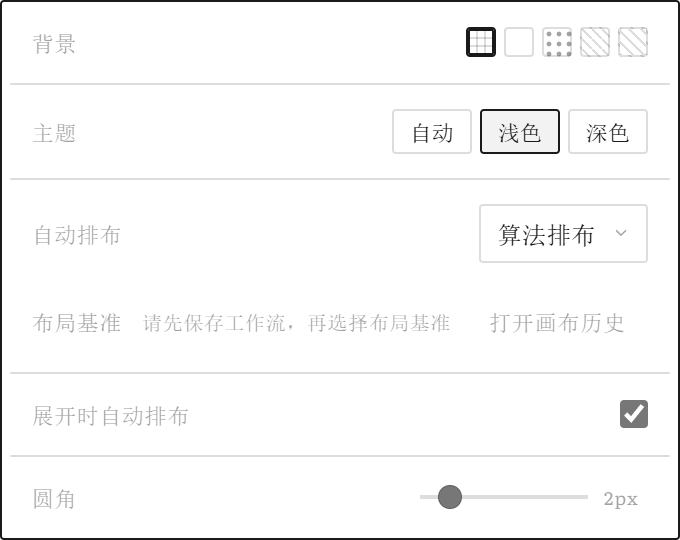
\includegraphics[width=0.5\textwidth]{style-menu.png}
\caption{样式菜单：背景、主题、排布、布局基准、画布历史、圆角}
\label{fig:style-menu}
\end{figure}

\section{画布}

画布是一张可以无限大的桌面。下面十个动作覆盖日常九成操作。

\begin{enumerate}
\item 放节点。点节点库的条目，或者按住拖到画布上松手。新节点落在视野中央或落点。
\item 连线。鼠标移到节点右侧的小圆点，按住拖到下一个节点左侧的圆点，松手成线。
\item 删除连线。点一下线，线变粗，按 Delete；框选可以一次删多条。
\item 选中。单击选一个，Shift 加单击加选，空白处拖方框框选。
\item 移动。拖节点本身；方向键逐像素微调，按着 Shift 步子更大。
\item 缩放与平移。滚轮缩放，空白处拖动平移，“\texttt{适应}”把所有节点装回屏幕，缩略图点哪去哪。
\item 撤销重做。菜单条的两个箭头，也可以按 Ctrl 加 Z。参数、挪位、连线都算一步。
\item 禁用节点。节点右上角的电源按钮。关掉以后不参与运行，下游失去唯一输入的节点也一起失效。
\item 复制粘贴。Ctrl 加 C 与 Ctrl 加 V，副本参数一样，位置稍微错开；剪贴板面板跨页面保存复制过的节点与文本。
\item 命名与注释。“\texttt{工作流命名}”给这一段起名字，运行记录和日志就用这个名字；“\texttt{注释}”节点不参与数据，只在画布上写说明。
\end{enumerate}

\begin{figure}[H]\centering
\begin{tikzpicture}[scale=0.95]
  \node[card=src,minimum width=3.0cm] (n1) at (0,0) {数据源};
  \node[card=prc,minimum width=3.0cm] (n2) at (4.6,0) {清洗};
  \draw[wire] (1.55,0) -- (3.05,0);
  \fill[src] (1.55,0) circle (2.4pt);
  \fill[prc] (3.05,0) circle (2.4pt);
  \draw[draw=ink!18,line width=0.4pt] (1.55,0) circle (5.5pt);
  \draw[draw=ink!18,line width=0.4pt] (3.05,0) circle (5.5pt);
  \node[micro,above=8pt] at (2.3,0.5) {拖住右侧圆点，落到左侧圆点};
\end{tikzpicture}
\caption{连线的两个圆点}
\label{fig:wire}
\end{figure}

快捷键都写在“\texttt{视图}”里的“\texttt{快捷键}”面板上：Enter 开合节点面板，L 进入连线模式，WASD 在节点之间跳，
空格加拖动平移，Delete 删除选中，Ctrl 加 Z 撤销，Ctrl 加 F 跳到大纲搜索。面板里列出的组合就是画布真正绑定的那一组。

\begin{figure}[H]\centering
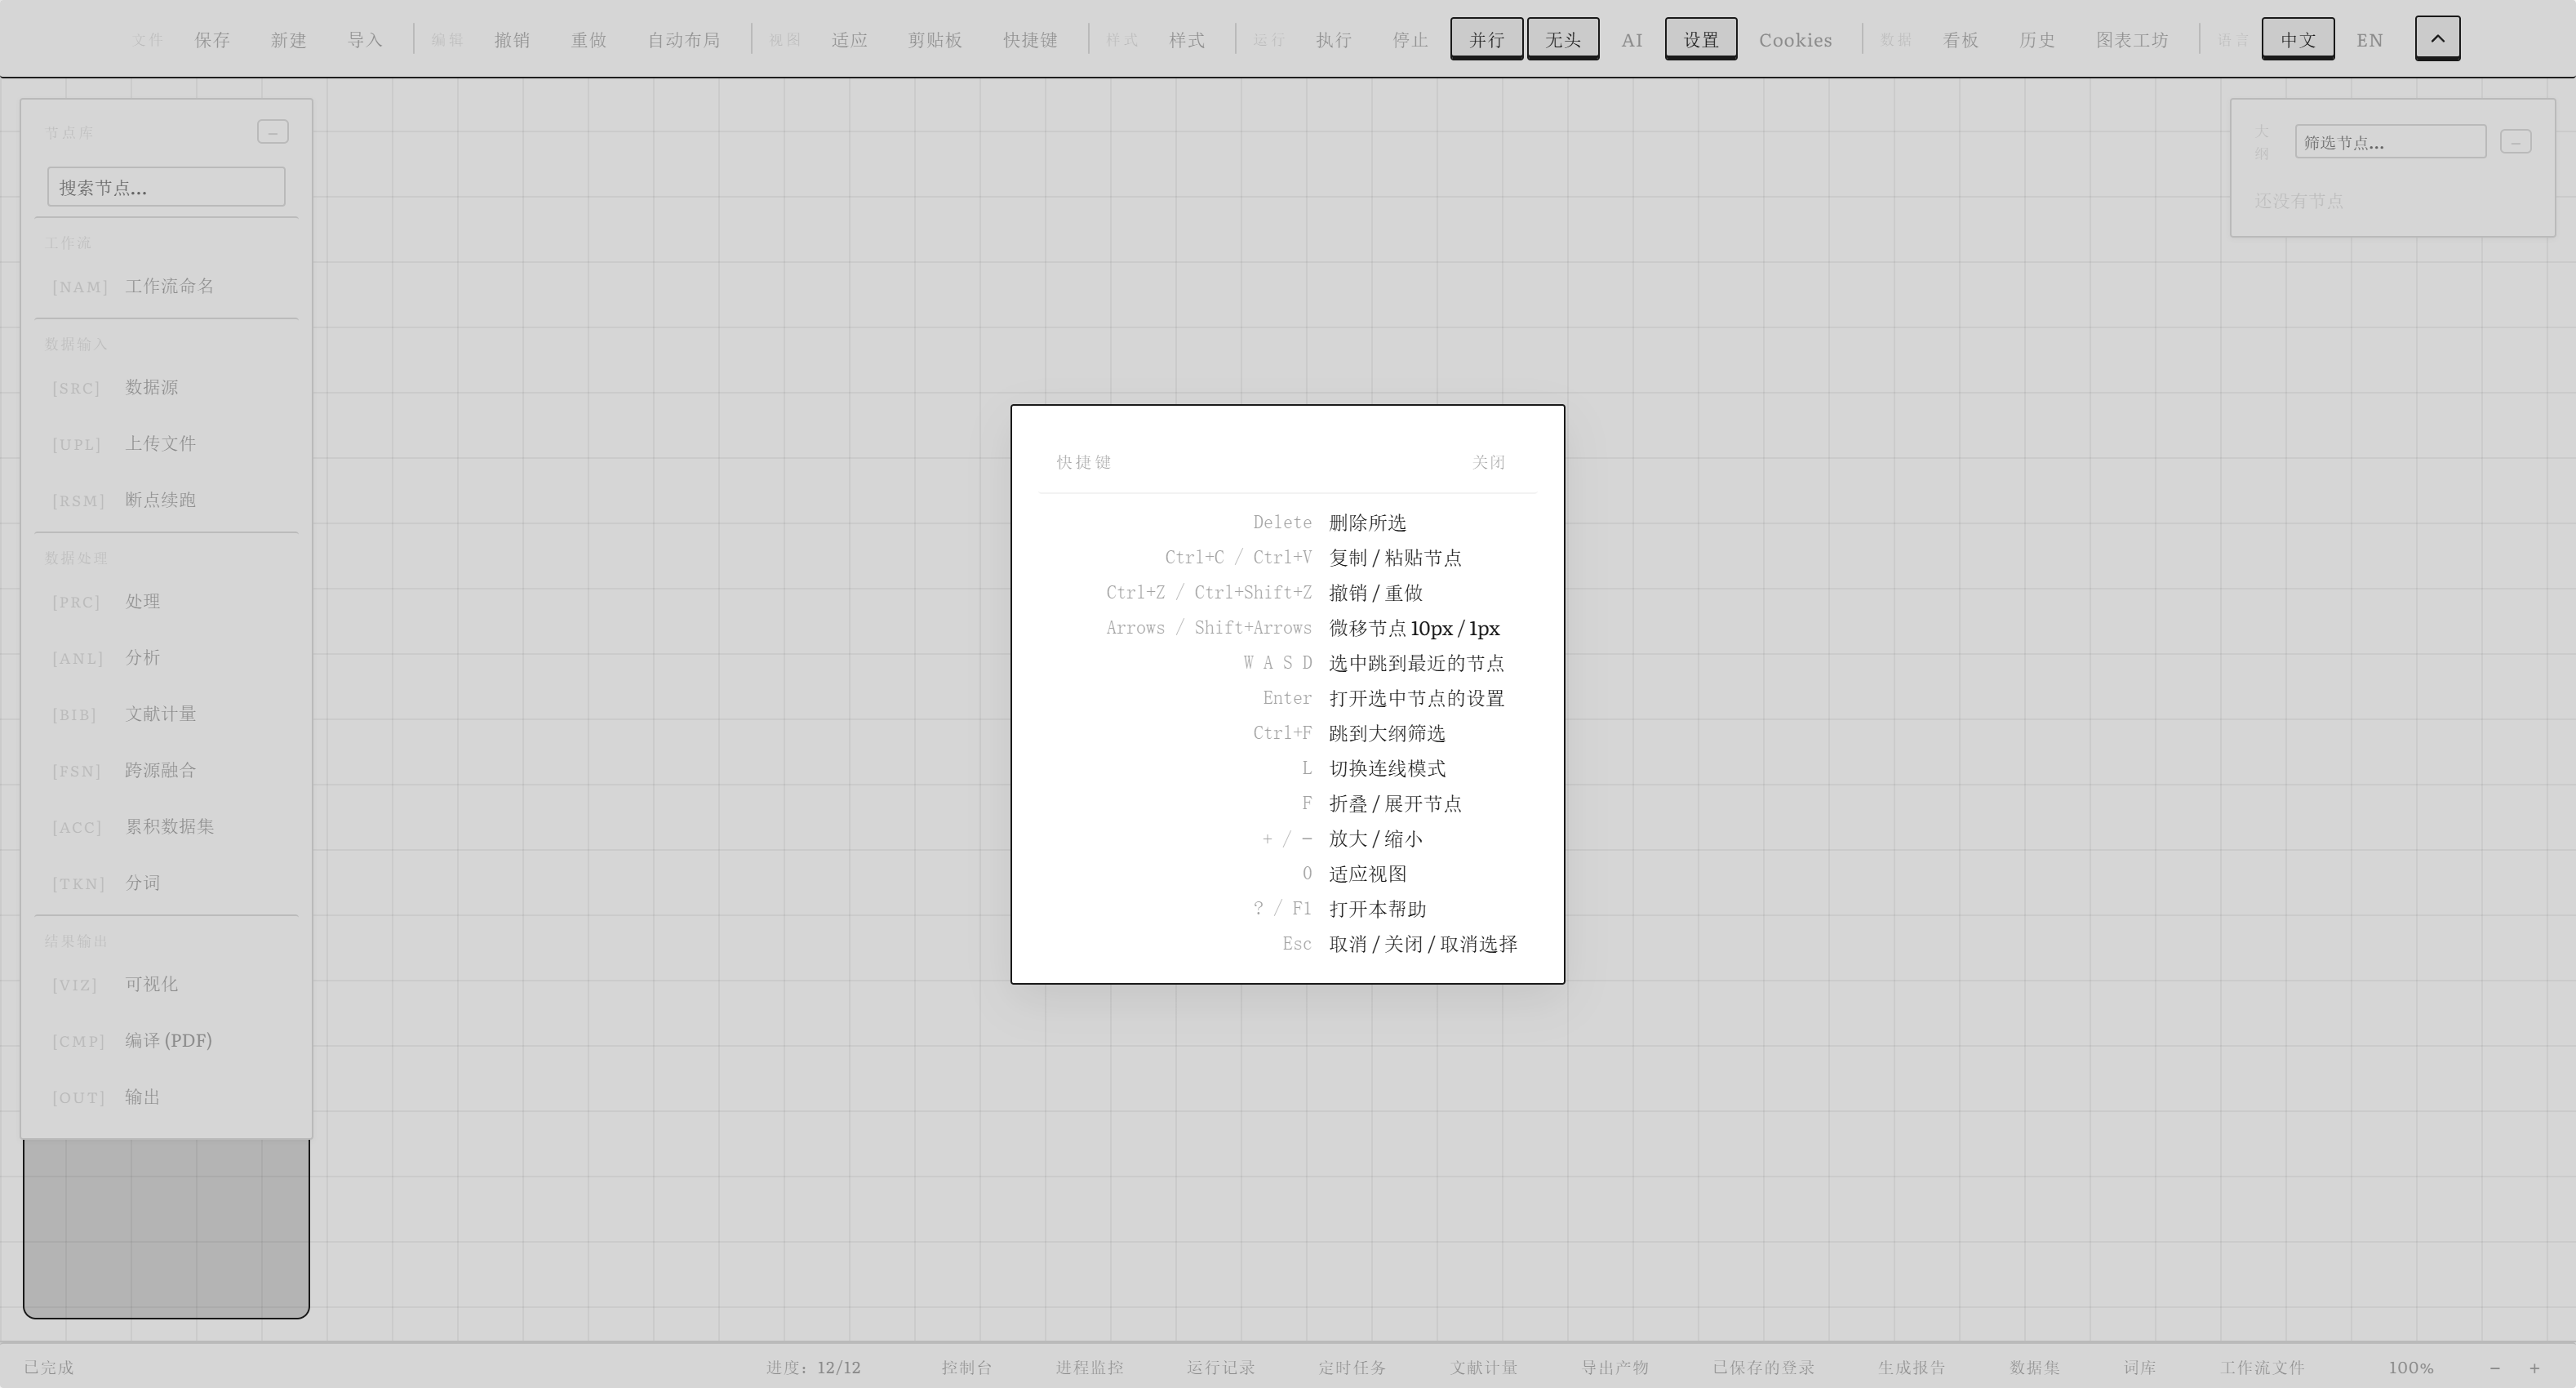
\includegraphics[width=0.72\textwidth]{shortcuts.png}
\caption{快捷键面板}
\label{fig:shortcuts}
\end{figure}

复制过的节点与文本进“\texttt{剪贴板}”抽屉，按标题或内容搜索，可以置顶、改名、单条删除或清空。抽屉里的内容重启浏览器还在。

\begin{figure}[H]\centering

\includegraphics[width=0.5\textwidth]{clipboard.png}
\caption{剪贴板抽屉}
\label{fig:clipboard}
\end{figure}

\section{节点与参数面板}

节点长得都一样：左边一道竖色条表示类型，标题下一行摘要写关键参数，右边三个按钮，依次是设置、删除、开关。

\begin{figure}[H]\centering
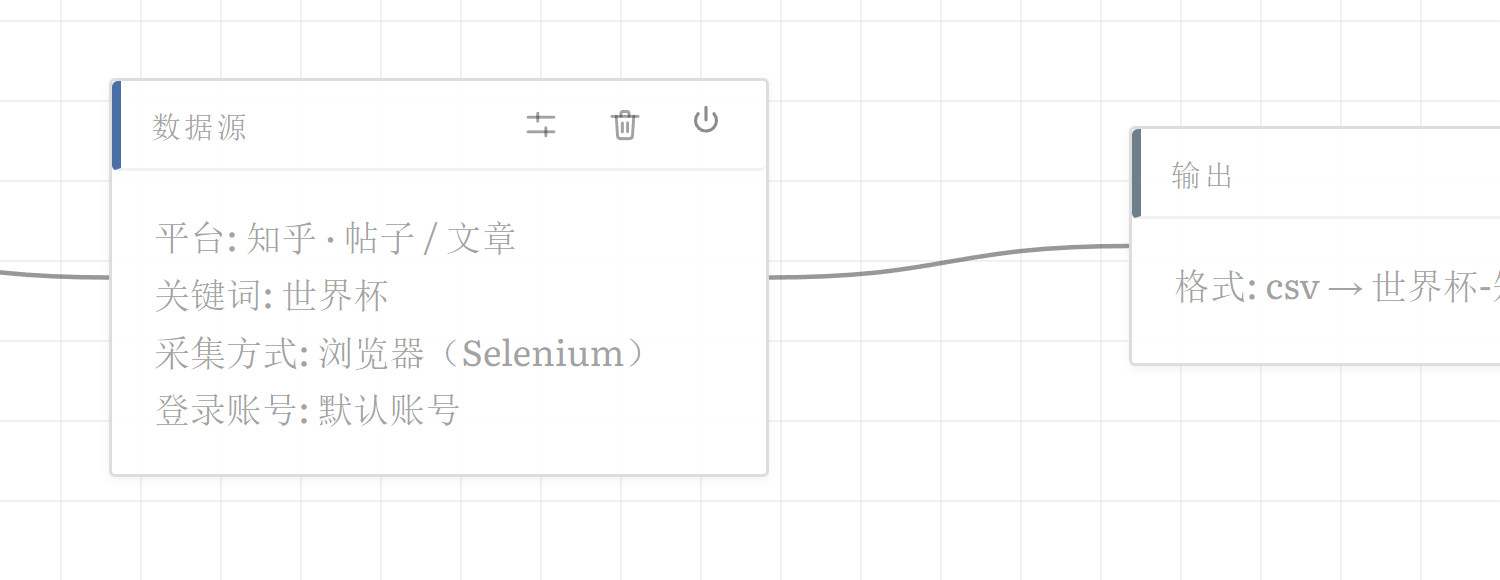
\includegraphics[width=0.72\textwidth]{node-closeup.png}
\caption{一个数据源节点：设置、删除、开关}
\label{fig:node}
\end{figure}

右上角还有状态角标。绿勾是完成或复用了以前的结果，转圈是在跑，红叉是没成功，灰色小点是没跑过或被关掉。
角标只反映运行库里的结论，不会把没跑过的画成成功。

点设置按钮打开右侧参数面板。面板结构固定：顶上写节点类型与标题，接着是这一段运行的校验结论，下面是主参数，最下面是预览按钮。
每一行都对应一个数据列或者一个行为；凡是需要先选一项才能继续的字段，面板不替你猜默认值，选错会按名字拒绝并列出可选项。

\begin{figure}[H]\centering
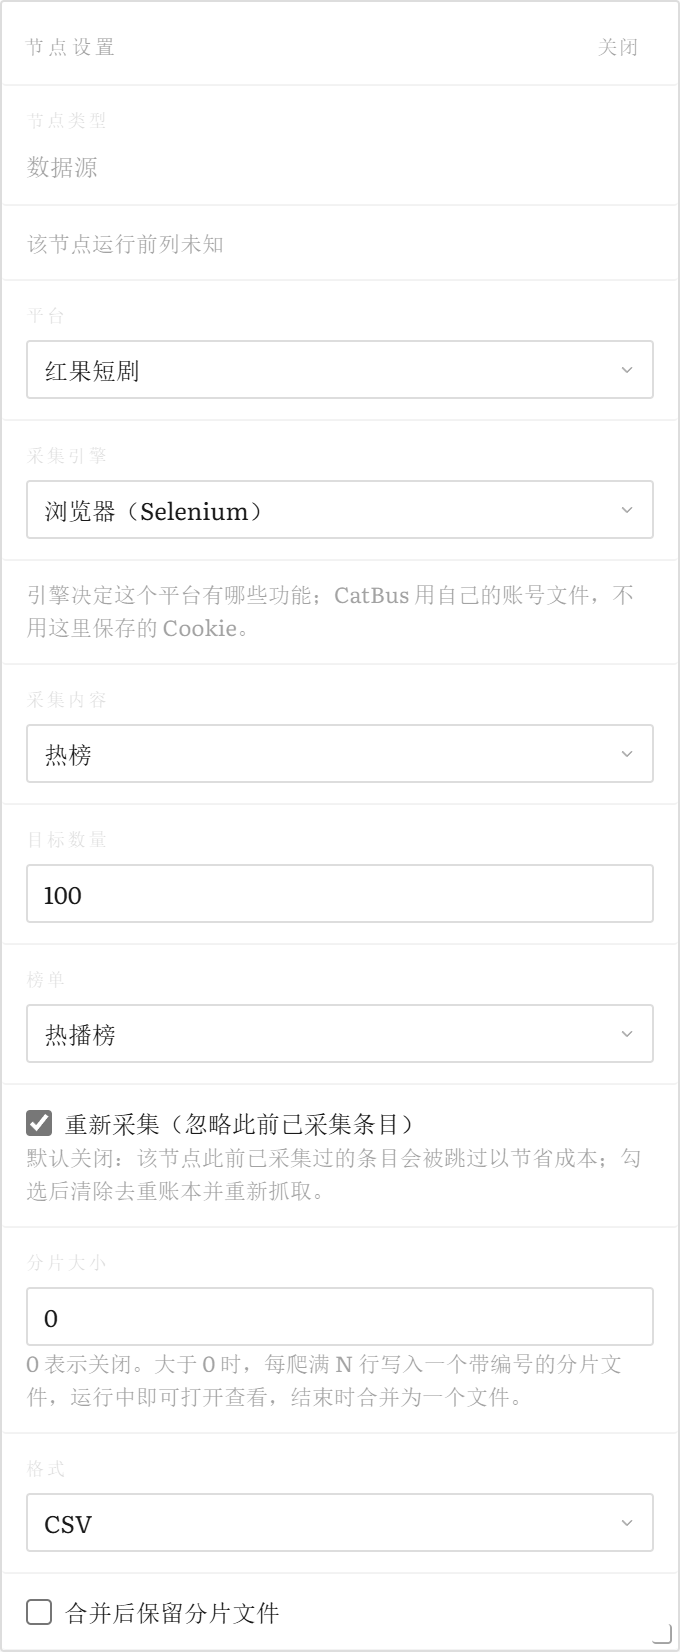
\includegraphics[width=0.31\textwidth]{panel-source.png}
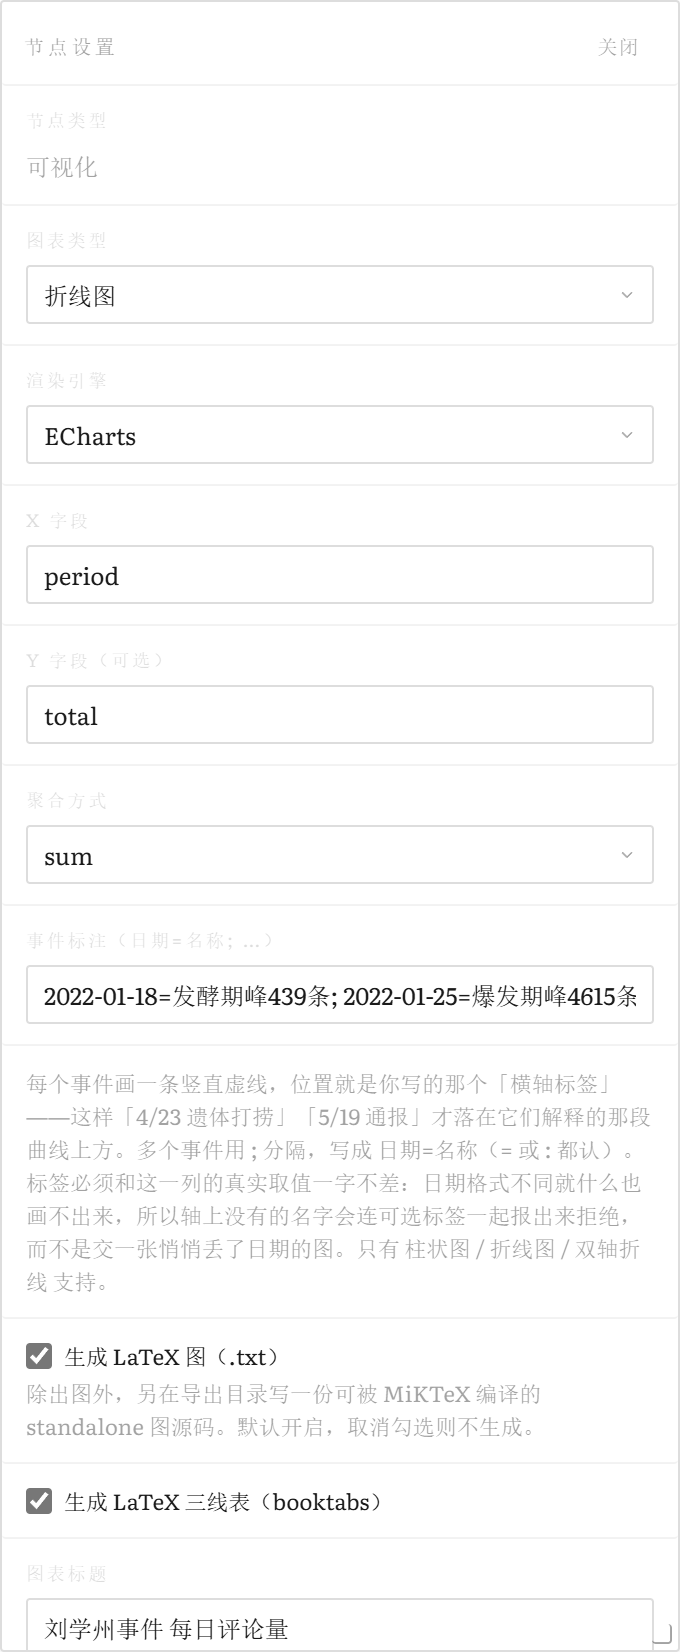
\includegraphics[width=0.31\textwidth]{panel-visualize.png}
\caption{左：数据源面板，平台、内容、数量、格式往下排；右：可视化面板，图表类型、引擎、字段、标题}
\label{fig:panels}
\end{figure}

摘要行值得常看。数据源写平台、内容、关键词或链接、账号；上传写文件名与行数；分析写操作与输出列；
可视化写图表类型与标题；输出写格式与文件名。看一眼摘要就知道这个节点是不是上次调好的那一份。

\section{节点类型}

节点库十三种，按数据流分工。

\begin{table}[H]\centering
\caption{节点类型}
\label{tab:nodes}
\small
\begin{tabularx}{\textwidth}{p{2.4cm}X}
\toprule
节点 & 作用 \\
\midrule
工作流命名 & 给这一条链贴名字，运行记录与日志用它 \\
数据源 & 采集一个平台的一种内容 \\
上传文件 & 读一张本地表，或挂一份已存数据集 \\
断点续跑 & 把历史运行的输出行收回来当输入，不重新采 \\
处理 & 分词、清洗、情感、倾向、关键词、聚类、实体、网暴、水军、相关、显著、异常 \\
分析 & 去重、筛选、选列、改名、排序、采样、聚合、关联、分箱、时间、阶段、主题、演化、预警 \\
文献计量 & 题录建网、指标、聚类、突现、变异、叠加 \\
跨源融合 & 多张表折成一份规范表 \\
累积数据集 & 每次追加新行到带版本的长期表 \\
可视化 & 三十种图与十四类文献图谱，另出 LaTeX 图源 \\
编译 & 把图和表用本机 xelatex 编成 PDF \\
输出 & 落成 CSV、JSON、Excel、文本、HTML、Markdown、Parquet 或 PDF \\
\bottomrule
\end{tabularx}
\end{table}

\begin{figure}[H]\centering
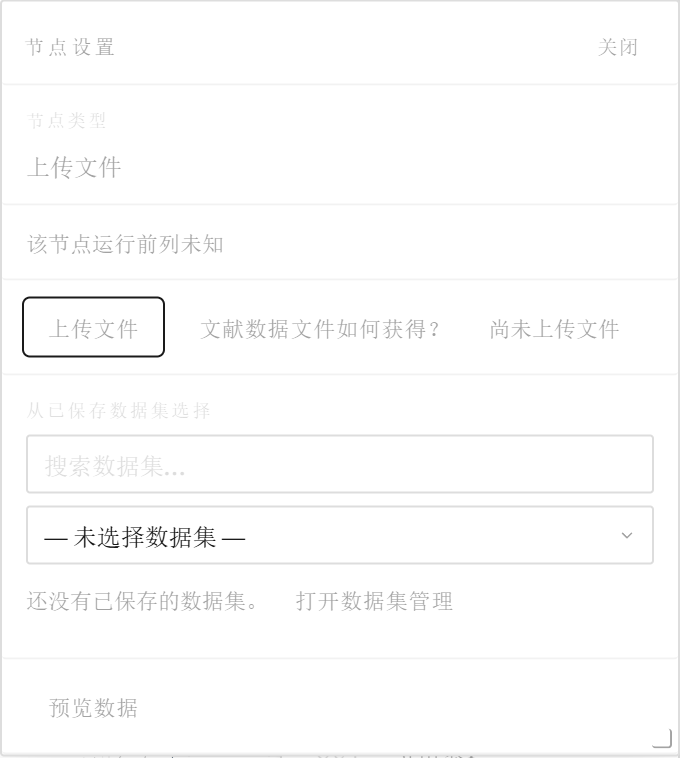
\includegraphics[width=0.31\textwidth]{panel-upload.png}
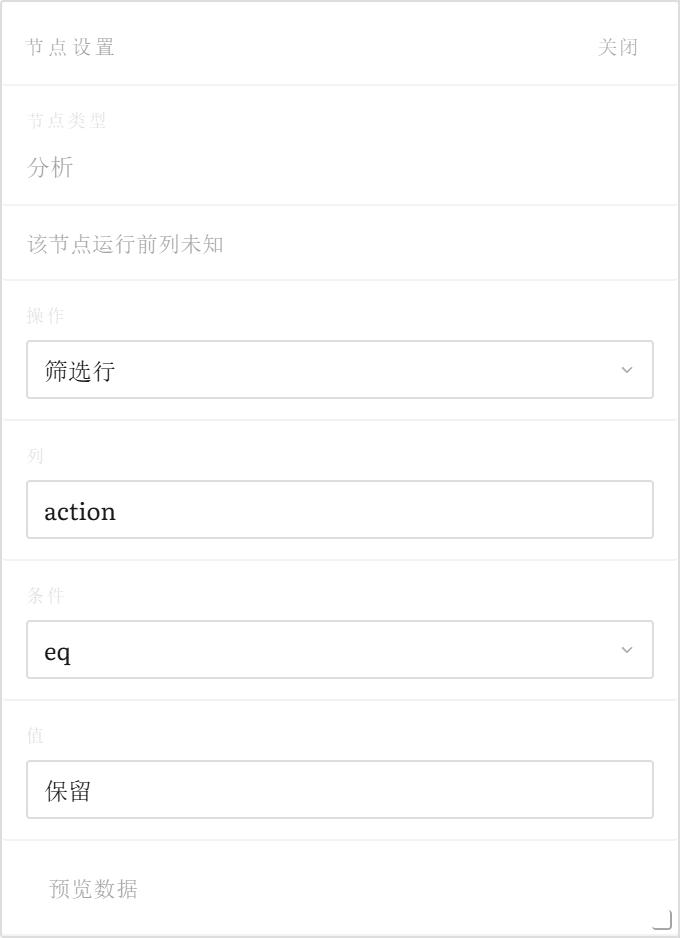
\includegraphics[width=0.31\textwidth]{panel-analysis.png}
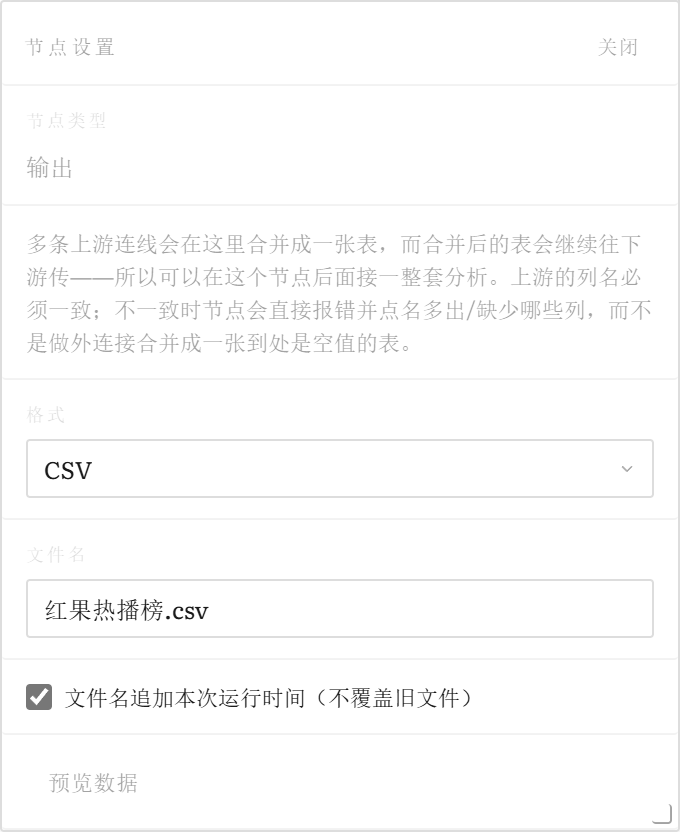
\includegraphics[width=0.31\textwidth]{panel-output.png}
\caption{上传、分析、输出三个面板，字段都按上游实际列名给候选项}
\label{fig:panels2}
\end{figure}

\section{运行一次}

按下“\texttt{执行}”先做三项检查：画布有没有环，每个节点参数齐不齐，这次要用的平台有没有登录状态。
任何一项不过就在开始前停下，控制台写清是哪个节点哪一项。

检查通过以后按连线顺序跑。一个节点可以接多个上游，上游表按列名取并集合并；也可以分给多个下游，各拿一份同样的输入。

服务同一时刻只跑一轮。忙的时候按钮变成“\texttt{排队运行}”，任务进队列，当前这轮结束自动开始。
勾了“\texttt{并行}”，几条互不相连的链同时跑；同一条链里的节点仍然一个接一个。
“\texttt{无头}”让浏览器在后台跑，不占桌面，第一次调试可以不开。

停止按钮把正在跑的与还没跑的节点一起停下。已经写进库的行保留，节点标成停止，不算失败，下次可以从那里接着做。

控制台按工作流分页签，实时输出，刷新页面会重新接上。日志同时写进运行库，事后在运行记录里还能翻到同一份。
进程监控列出服务内正在跑的后台线程，采集卡住时用它看是哪一条。

\begin{figure}[H]\centering
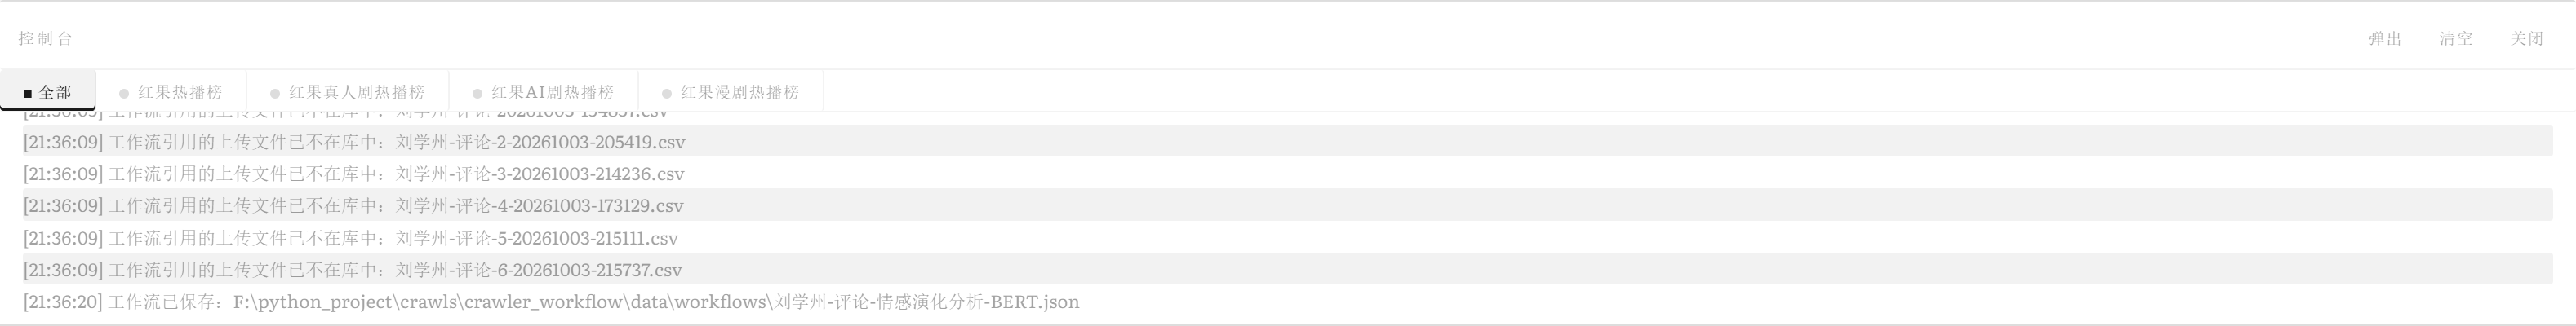
\includegraphics[width=0.98\textwidth]{console.png}
\caption{控制台：工作流页签、级别过滤、搜索、导出}
\label{fig:console}
\end{figure}

\section{从零做一次}

这一节不采集，只用一张现成的表格走完整条链：上传、分析、出图、看数据、找文件。全程十分钟，不需要登录任何平台。

\subsection{第一步\quad 新建并命名}

菜单条点“\texttt{新建}”，画布清空，状态栏节点数为零。节点库点“\texttt{工作流命名}”，它落在画布中央。
打开设置，在“\texttt{工作流名称}”里写“\texttt{示例 评论情感}”。运行记录和日志以后就用这个名字。

\subsection{第二步\quad 准备表格}

任意一张两列的 CSV，一列分类，一列文本。这一节用二十来条餐厅评论，列名是“\texttt{城市}”与“\texttt{评论}”。
第一行必须是表头，编码用 UTF-8。表格不必大，二十行能看出结果，真实项目几千行流程一样。

\subsection{第三步\quad 上传}

节点库点“\texttt{上传文件}”，放在命名节点右边，打开设置。

\begin{enumerate}
\item 点“\texttt{选择文件}”，挑刚才那张 CSV。
\item 传完面板写文件名、列数、行数，并列出识别到的列名。
\item 文本列选“\texttt{评论}”，下游据此知道读哪一列。
\end{enumerate}

Excel 一次只读一张工作表，多张非空的表会拒绝并列出表名。

\subsection{第四步\quad 分析}

节点库点“\texttt{处理}”，接在上传右边，打开设置。

\begin{enumerate}
\item 操作选“\texttt{情感极性}”，输出标签与零到一的分数。
\item 文本列填“\texttt{评论}”。
\item 分析模式选 \texttt{SnowNLP}，不联网、不占显存。
\item 两个阈值保持默认：正面零点六，负面零点四，中间算中性。
\end{enumerate}

面板底部点“\texttt{预览数据}”，先确认列没选错再往下走。

\subsection{第五步\quad 可视化}

节点库点“\texttt{可视化}”，接在分析节点右边。

\begin{enumerate}
\item 图表类型选“\texttt{柱状图}”，渲染引擎保持 \texttt{ECharts}。
\item 横轴字段选 \texttt{sentiment}，也就是上一步写出的标签列。
\item 聚合方式选“\texttt{计数}”，值字段留空。
\item 图表标题写“\texttt{各情感倾向的评论数}”。
\end{enumerate}

“\texttt{生成 LaTeX 图}”与“\texttt{生成 LaTeX 三线表}”默认勾着，跑完导出目录会多一份可编译的图源。

\subsection{第六步\quad 连线}

三个节点从左到右摆好，用右侧圆点接到下一个节点左侧圆点。命名节点也要连到上传节点，否则运行前会提示它没有下游。

\begin{figure}[H]\centering
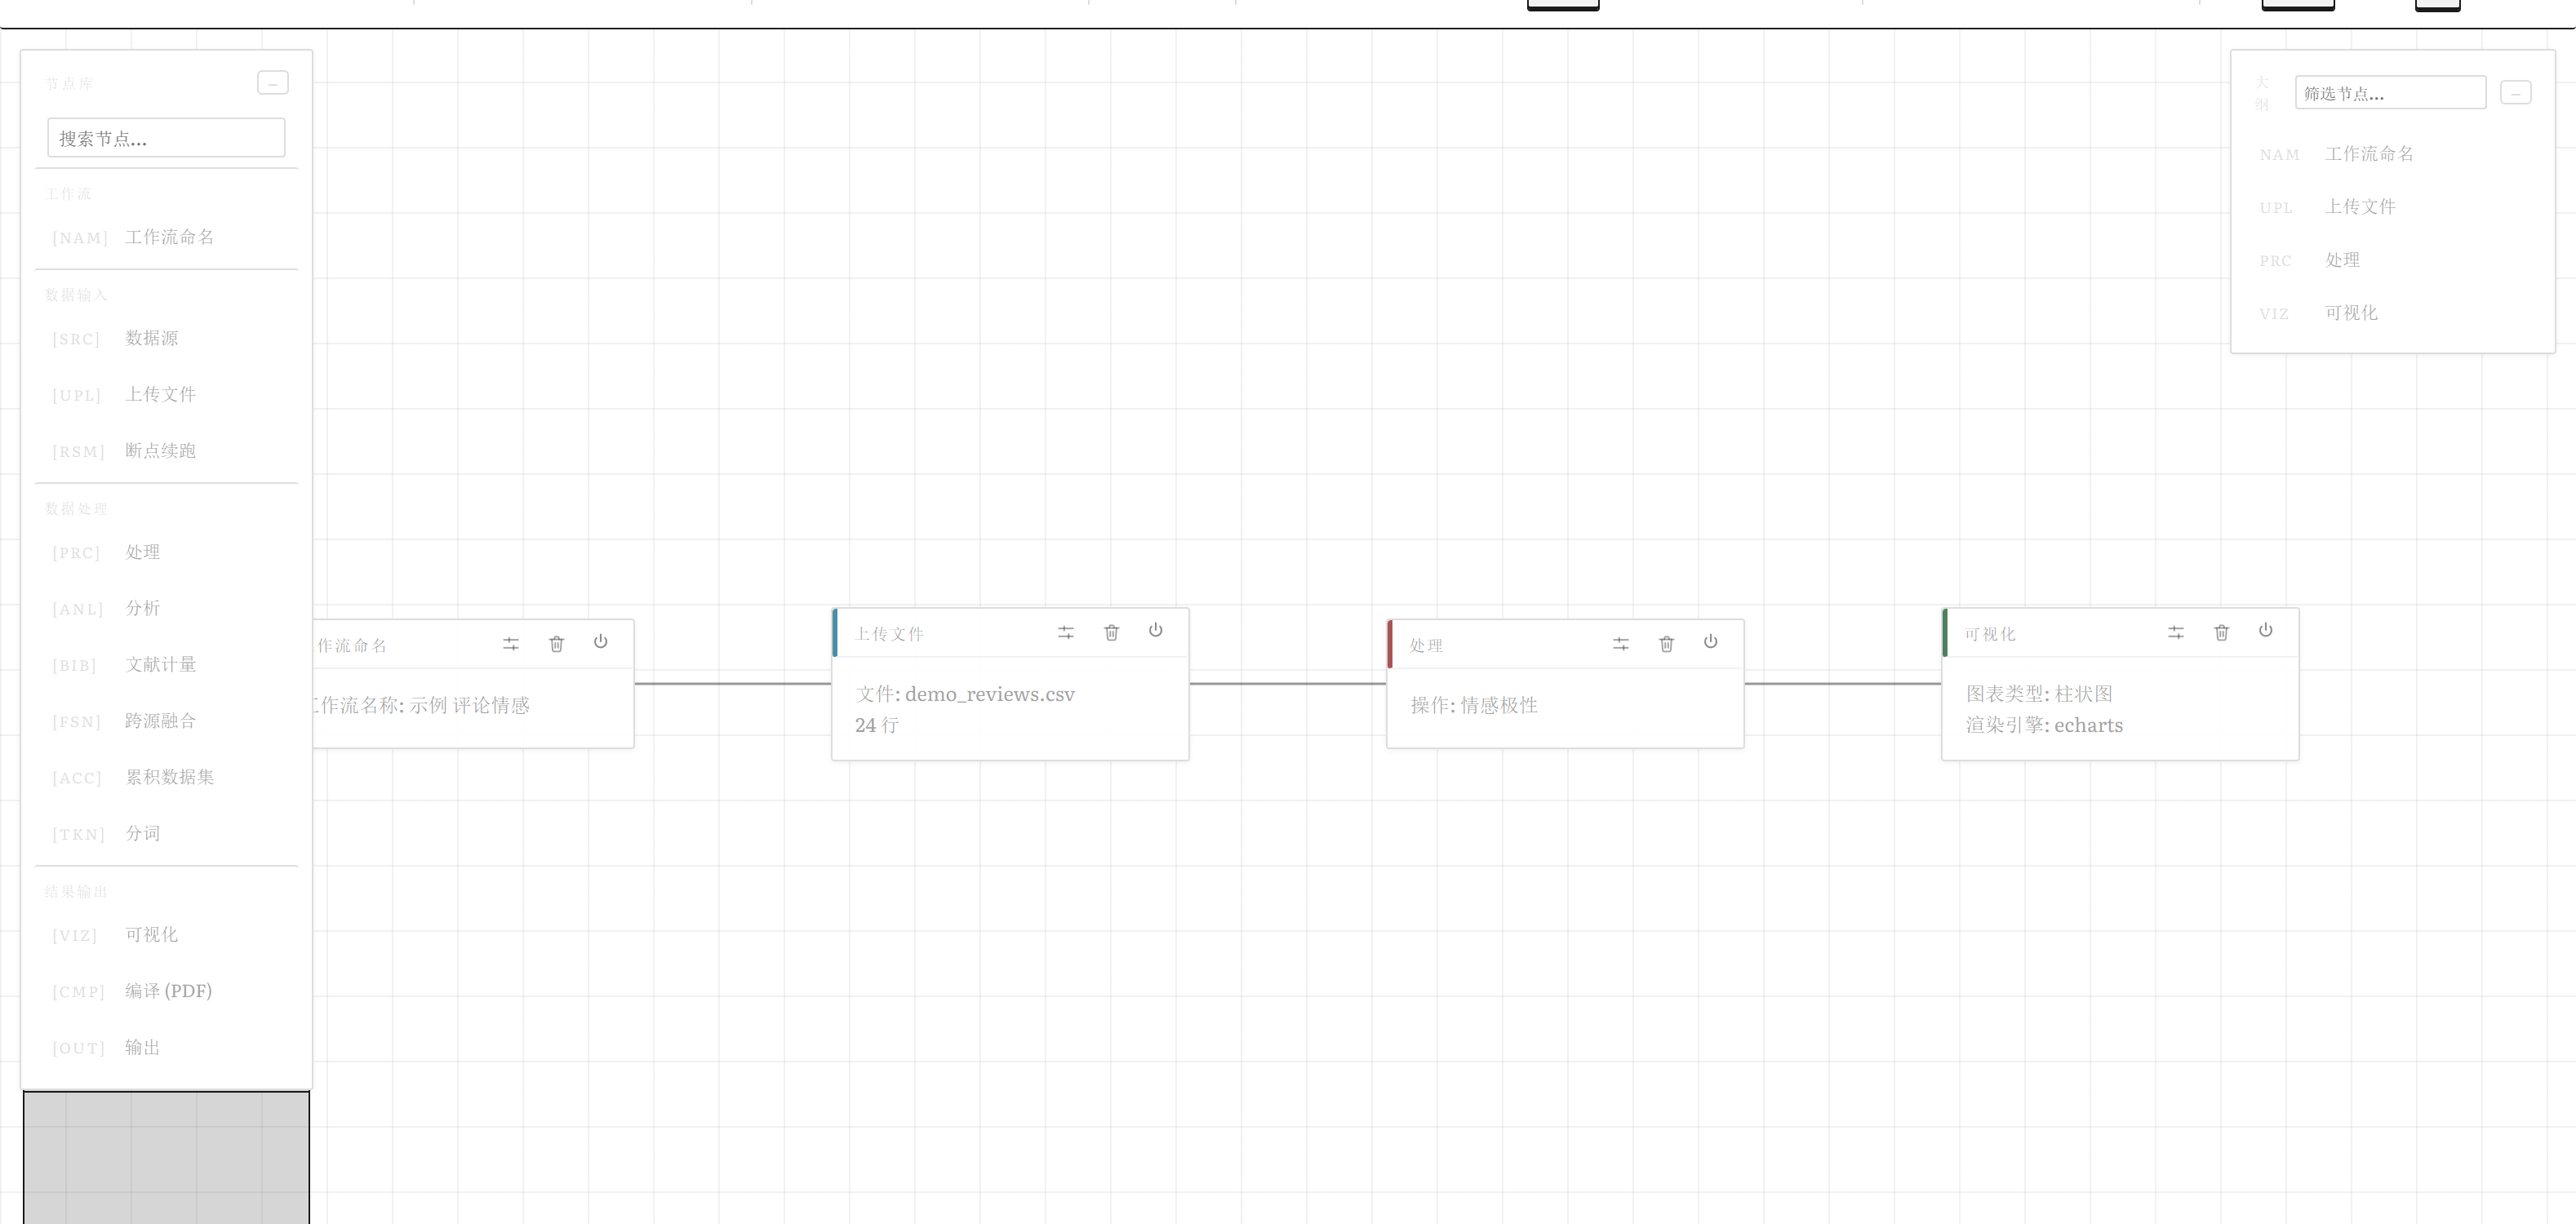
\includegraphics[width=0.9\textwidth]{demo-canvas.png}
\caption{最小的一条工作流：命名、上传、分析、可视化}
\label{fig:demo-canvas}
\end{figure}

\subsection{第七步\quad 保存}

菜单条点“\texttt{保存}”，起名“\texttt{示例-评论情感}”。保存的是画布本身：节点位置、参数、连线、视角。
数据集不存进工作流，工作流只记它的编号，换机器时数据目录要一起搬。

\subsection{第八步\quad 执行}

点“\texttt{执行}”。控制台先写发现了几个节点，再逐个写正在执行哪个、完成几个。二十多行数据几秒钟跑完。
分析节点会打印实际用的模式，可视化节点会打印画了多少行、生成了哪些文件，最后一行是运行结束与完成节点数。

\subsection{第九步\quad 看图}

回到可视化节点，点设置底部的“\texttt{预览图表}”。图在浮层里出现，顶上四个按钮分别是全屏、存为图片、存为 SVG、关闭；
底部还能复制或下载 LaTeX 图源、把图编译成 PDF、复制或下载三线表。

\begin{figure}[H]\centering
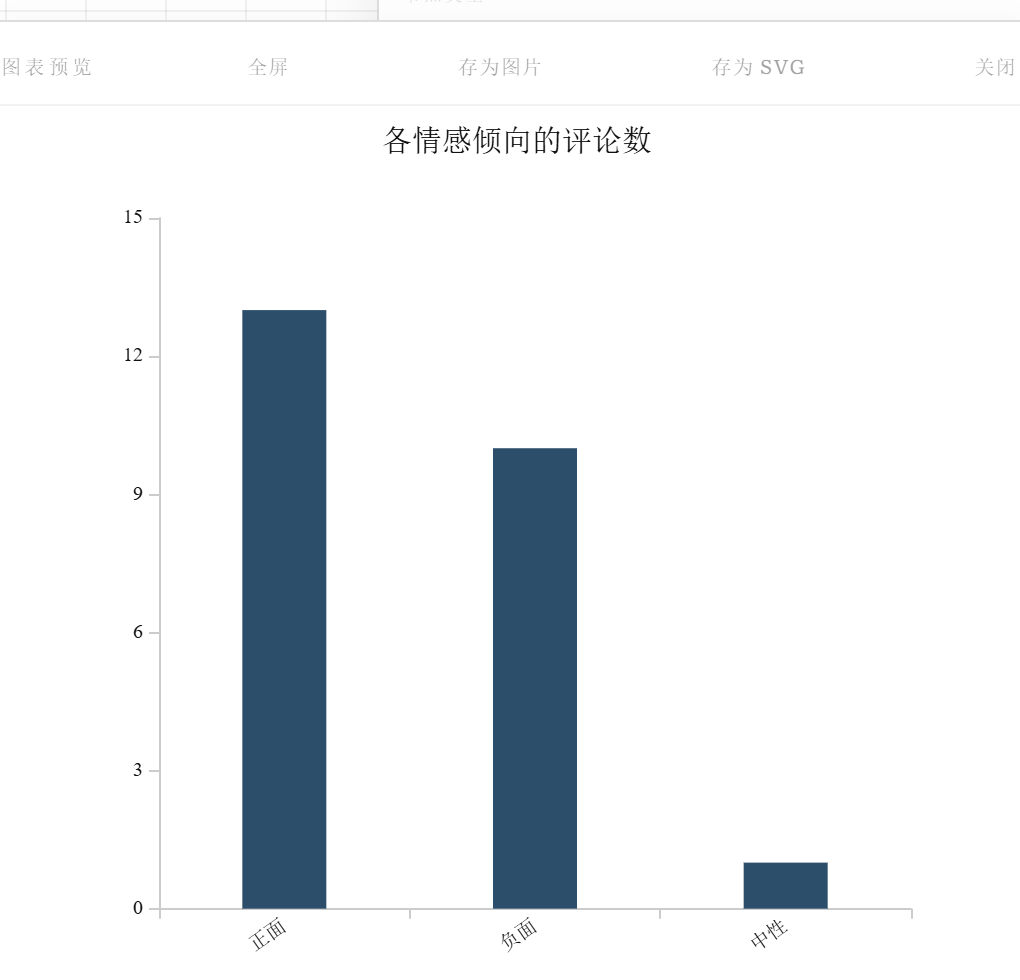
\includegraphics[width=0.72\textwidth]{demo-chart.png}
\caption{预览图表：论文样式的柱状图，正面十三、负面十、中性一}
\label{fig:demo-chart}
\end{figure}

坐标轴只留左边与下面两条，网格很浅，柱条是直角，分类多时横轴自动斜排，每一格都显示，不为避让丢标签。

\subsection{第十步\quad 翻数据}

回到分析节点，点“\texttt{预览数据}”。表头写着行数与列数，底部能翻页，分析结果就在原文右边多出的两列里。

\begin{figure}[H]\centering
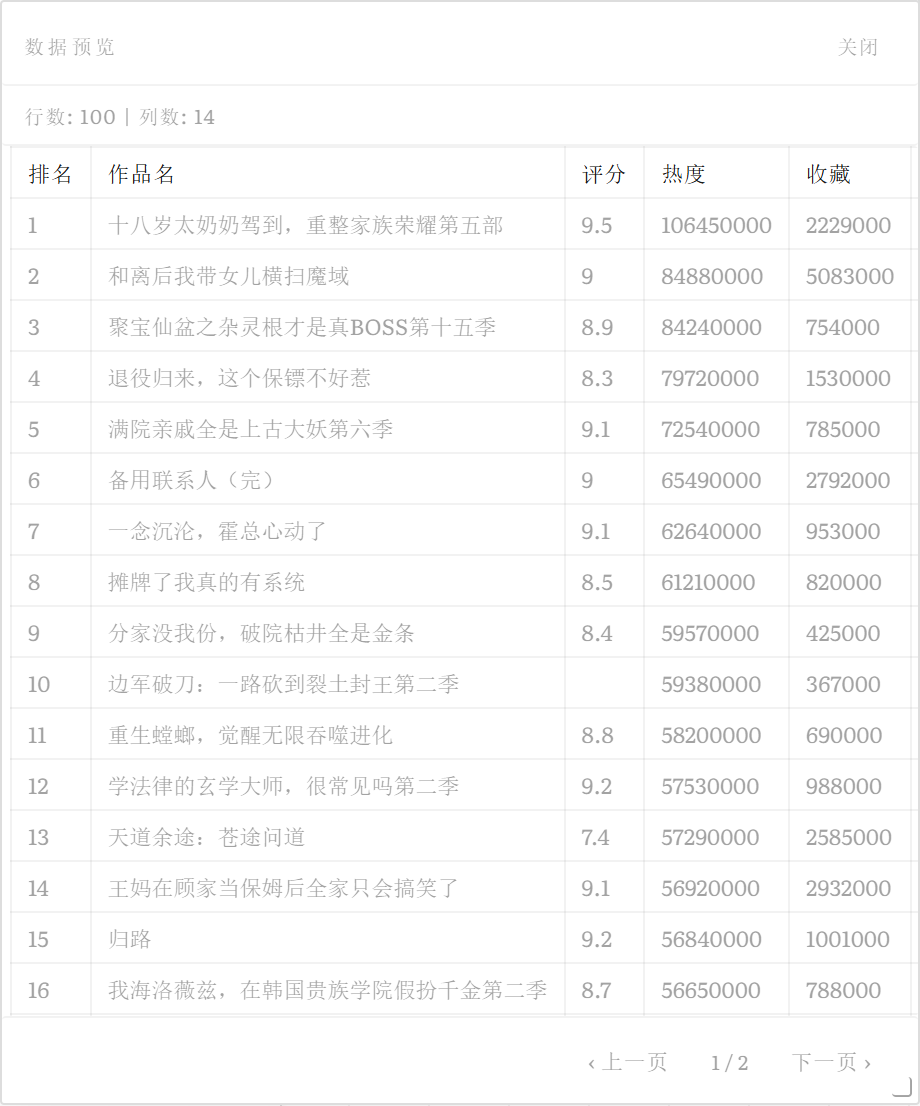
\includegraphics[width=0.72\textwidth]{data-preview.png}
\caption{数据预览：行数、列数、翻页，任何一步都能这样翻}
\label{fig:data-preview}
\end{figure}

\subsection{第十一步\quad 找文件与查记录}

底部点“\texttt{导出产物}”，这次运行写下的文件都在：图表的 PNG、LaTeX 图源、三线表。每一行能下载、删除、复制路径。

\begin{figure}[H]\centering
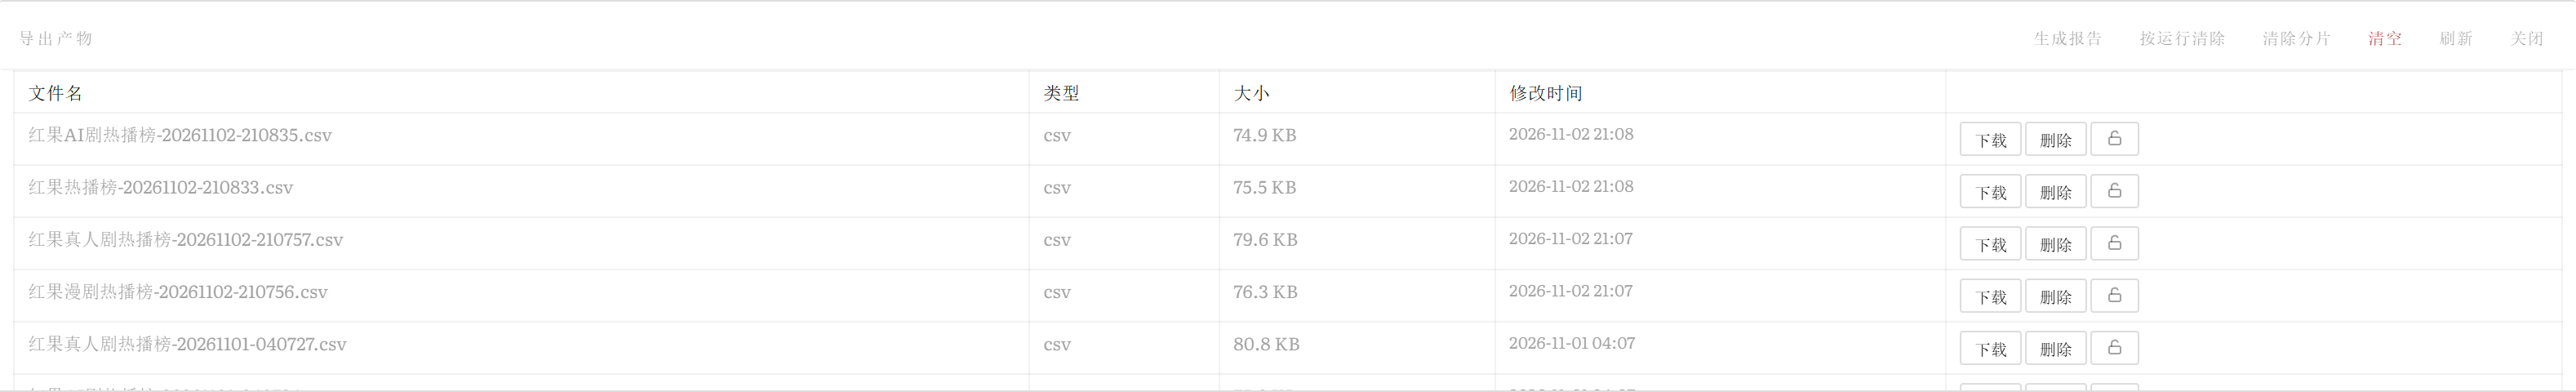
\includegraphics[width=0.96\textwidth]{exports-panel.png}
\caption{导出产物，按运行归档}
\label{fig:exports-panel}
\end{figure}

底部点“\texttt{运行记录}”，这一行写着状态、节点数、行数、开始时间与耗时。右边的按钮能载入这次结果、打开完整日志、生成报告、删除记录。

到这里，建画布、填参数、连线、保存、运行、看图、翻数据、找文件都走了一遍。后面的复杂工作流都是在这几步上叠功能。

\section{采集}

采集节点只有一个，选项很多。选平台，选采集内容，填目标数量，选格式，剩下的交给程序。
平台之间的差别收在一张表里，面板只显示这个平台真正支持的那几项。

\begin{table}[H]\centering
\caption{各平台能采集的内容}
\label{tab:platforms}
\small
\begin{tabularx}{\textwidth}{p{2.6cm}X}
\toprule
平台 & 可选内容 \\
\midrule
知乎 & 关键词帖子与文章、某作者的作品、热榜、评论 \\
微博 & 关键词帖子、某作者的作品、热搜、评论 \\
小红书 & 关键词笔记、某作者的笔记、评论 \\
微信公众号 & 关键词文章正文 \\
哔哩哔哩 & 关键词视频、某作者的作品、热榜、评论 \\
抖音 & 某作者的作品、热榜、评论 \\
红果短剧 & 四个榜单、评论（仅 Windows 桌面） \\
中国知网 & 文献检索结果，按篇数导出 \\
YouTube & 关键词视频、频道作品、评论 \\
X & 关键词帖子、某作者的作品、评论 \\
Instagram & 只能保存登录状态，采集未接入 \\
\bottomrule
\end{tabularx}
\end{table}

采集引擎有两套。一套是浏览器，用 Selenium 驱动本机 Chrome；另一套是 CatBus，一个独立的外部采集器，
走自己的适配器与账号文件。两套后端能采什么、输出哪些列，都读各自的清单，选到不支持的组合会置灰并写明原因。

浏览器这套要登录状态。一个平台一个账号对应一份 Cookie 快照加一个独立的浏览器目录，对站点来说就是一台连续的设备。
默认那份登录也有名字，叫默认账号。采集节点的账号下拉列出当前存了登录的账号。

按下执行前会做一次登录预检：用这次真要用的浏览器打开平台首页，看它还认不认这份登录。跳到登录页就拦下来并点名平台。
因为网络慢、验证码、站点忙而没法判断的情况不拦，只记一笔，让你自己决定。预检可以关，关掉后由采集自己撞墙再报错。

采集支持分批落库。节点里填分片大小，每满 N 行先写一个带编号的文件，运行中就能打开看，结束时合成一份。
分片文件名可以带采集时间或者本次创建时间，跑第二遍不覆盖第一遍。

采集也支持上游喂任务。上游是一张表时，在节点里指定一列，程序逐行取这一列的链接或名字去采。
这是批量补抓评论最省事的做法，热榜转评论那一节会完整走一遍。

采集结束时报一个数。站点提前到底就按站点自己的话结束，并说明第几页到底；没到目标数量就停下时，控制台写清为什么停，
不会把短表当成长表交给你。

\section{保存登录}

要采带登录态的内容，先存一份登录，存一次以后一直用。

\begin{enumerate}
\item 菜单条点“\texttt{Cookies}”，打开登录设置。左边选平台，右边是这一份登录的字段。
\item “\texttt{账号}”留空就是默认账号，填一个新名字则另存一份，用来对付限流或换号。
\item 点“\texttt{浏览器生成}”，程序弹出一个 Chrome 窗口，你在里面扫码或输密码登录，登录完回到本面板点“\texttt{已完成登录}”，Cookie 自动收下来。
\item 也可以把浏览器导出的 Cookie JSON 粘进大框，点“\texttt{保存 Cookies}”。
\item 点“\texttt{验证 Cookie}”，程序打开平台首页问一句还认不认，认就写可用，不认就写失效。
\end{enumerate}

\begin{figure}[H]\centering
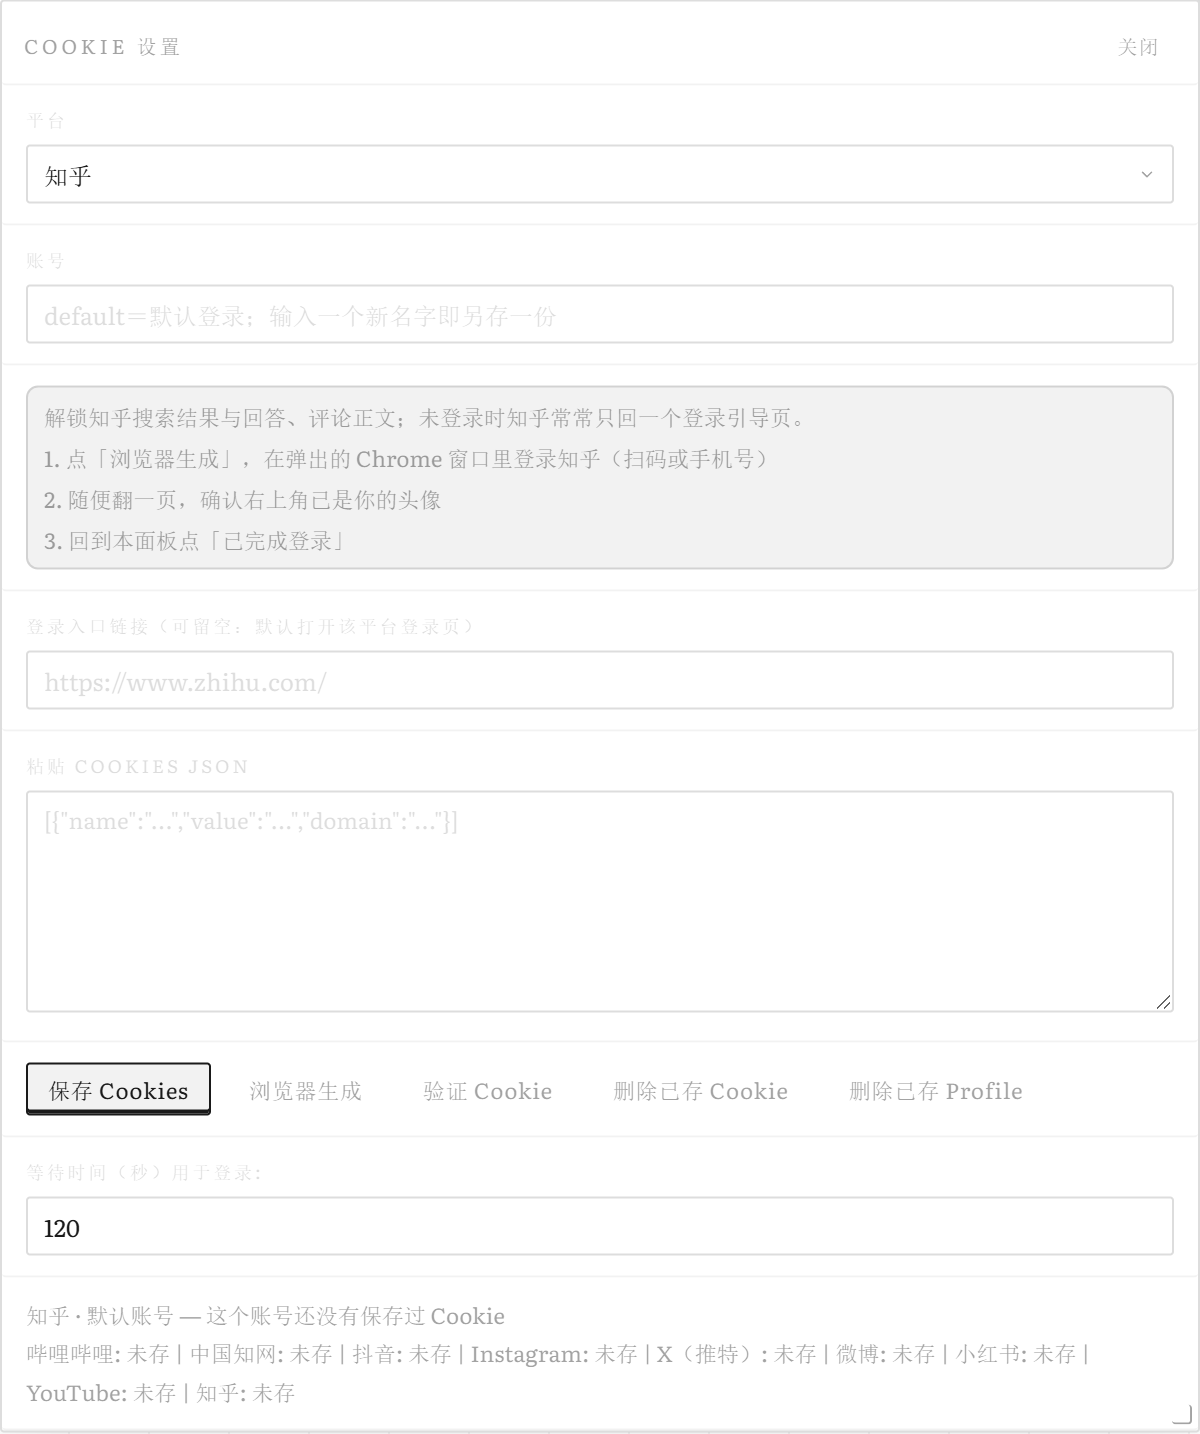
\includegraphics[width=0.56\textwidth]{cookie-dialog.png}
\caption{登录设置：平台、账号、登录入口、粘贴区与四个操作按钮}
\label{fig:cookie-dialog}
\end{figure}

面板底部一行是各平台当前账号的状态，未存、可用、失效一眼可见。存好的登录出现在底部“\texttt{已保存的登录}”表里，
一行一个平台加账号，写着条数与存入时间，每行能重命名、删 Cookie、删浏览器目录。

\begin{figure}[H]\centering

\includegraphics[width=0.86\textwidth]{cookies.png}
\caption{已保存的登录，一行一个平台加账号}
\label{fig:cookies}
\end{figure}

两个删除不一样。删 Cookie 只删那份快照，浏览器目录里的登录态还在，下次采集仍可能是登录的；删 Profile 才是把那台设备登出。
写论文前如果换过账号，两个都要清，免得采到上一个账号的视角。

采集节点里的“\texttt{登录账号}”就是这张表里的名字。选了哪份就用哪份，预检也会用它打开首页核对一遍。

\section{实战一\quad 红果短剧四个热播榜}

这一段从空白画布做出一条能跑的采集链，得到四份 CSV：热播榜、真人剧、AI 剧、漫剧，每个一百条。
红果只能在本机桌面上采，别的系统上这个平台会按名字拒绝。

\subsection{建链}

菜单条点“\texttt{新建}”。节点库拖出“\texttt{工作流命名}”，设置里填“\texttt{红果热播榜}”。
右边放“\texttt{数据源}”，打开设置依次填：

\begin{enumerate}
\item 平台“\texttt{红果短剧}”，采集引擎“\texttt{浏览器}”，采集内容“\texttt{热榜}”。
\item 目标数量 \texttt{100}。这是上限，站点只有五页就写到一百条为止。
\item 榜单选“\texttt{热播榜}”，另外三个是真人剧、AI 剧、漫剧。
\item 重新采集打勾，分片大小填 \texttt{0}，格式 \texttt{CSV}。
\end{enumerate}

右边再放“\texttt{输出}”：操作“\texttt{保存}”，格式 \texttt{CSV}，文件名“\texttt{红果热播榜.csv}”，勾上“\texttt{文件名追加本次运行时间}”。

\begin{figure}[H]\centering
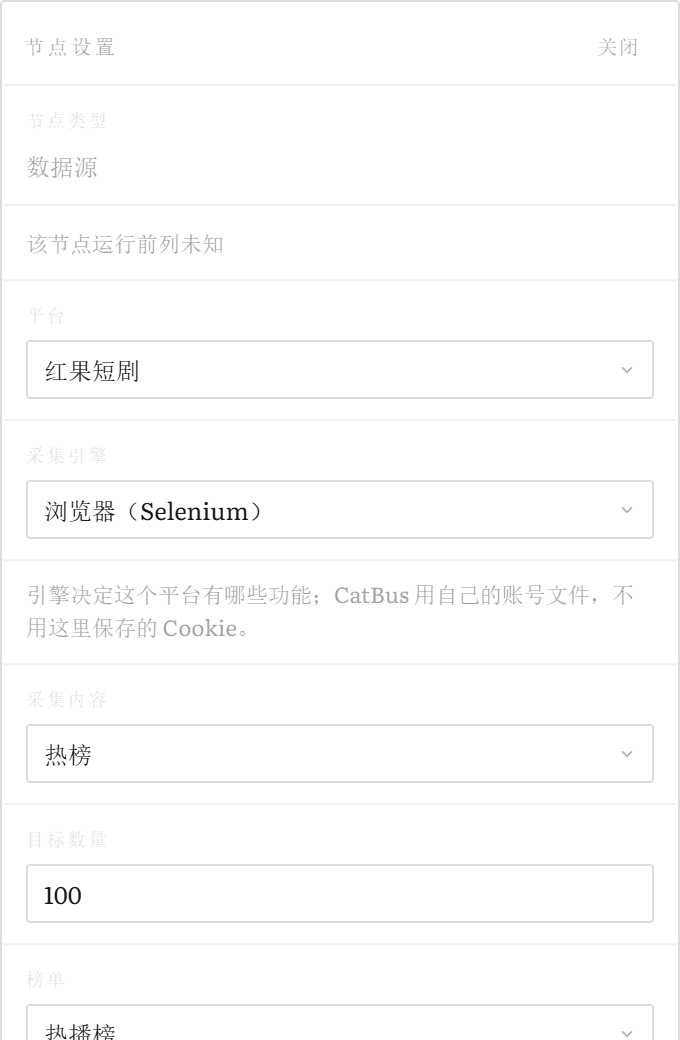
\includegraphics[width=0.31\textwidth]{hg-source.png}
\caption{红果数据源：平台、内容、数量、榜单、重新采集、格式}
\label{fig:hg-source}
\end{figure}

从命名节点右侧圆点拖到数据源左侧，再从数据源拖到输出左侧。两条线一接，这条链就成立。

\subsection{复制成四条}

把三个节点框选，Ctrl 加 C，Ctrl 加 V 三次。每条链改三处：名字、榜单、文件名。
四条链互不相连，摆成四行，画布就是下图。节点上的绿勾是上一次跑完留下的。

\begin{figure}[H]\centering
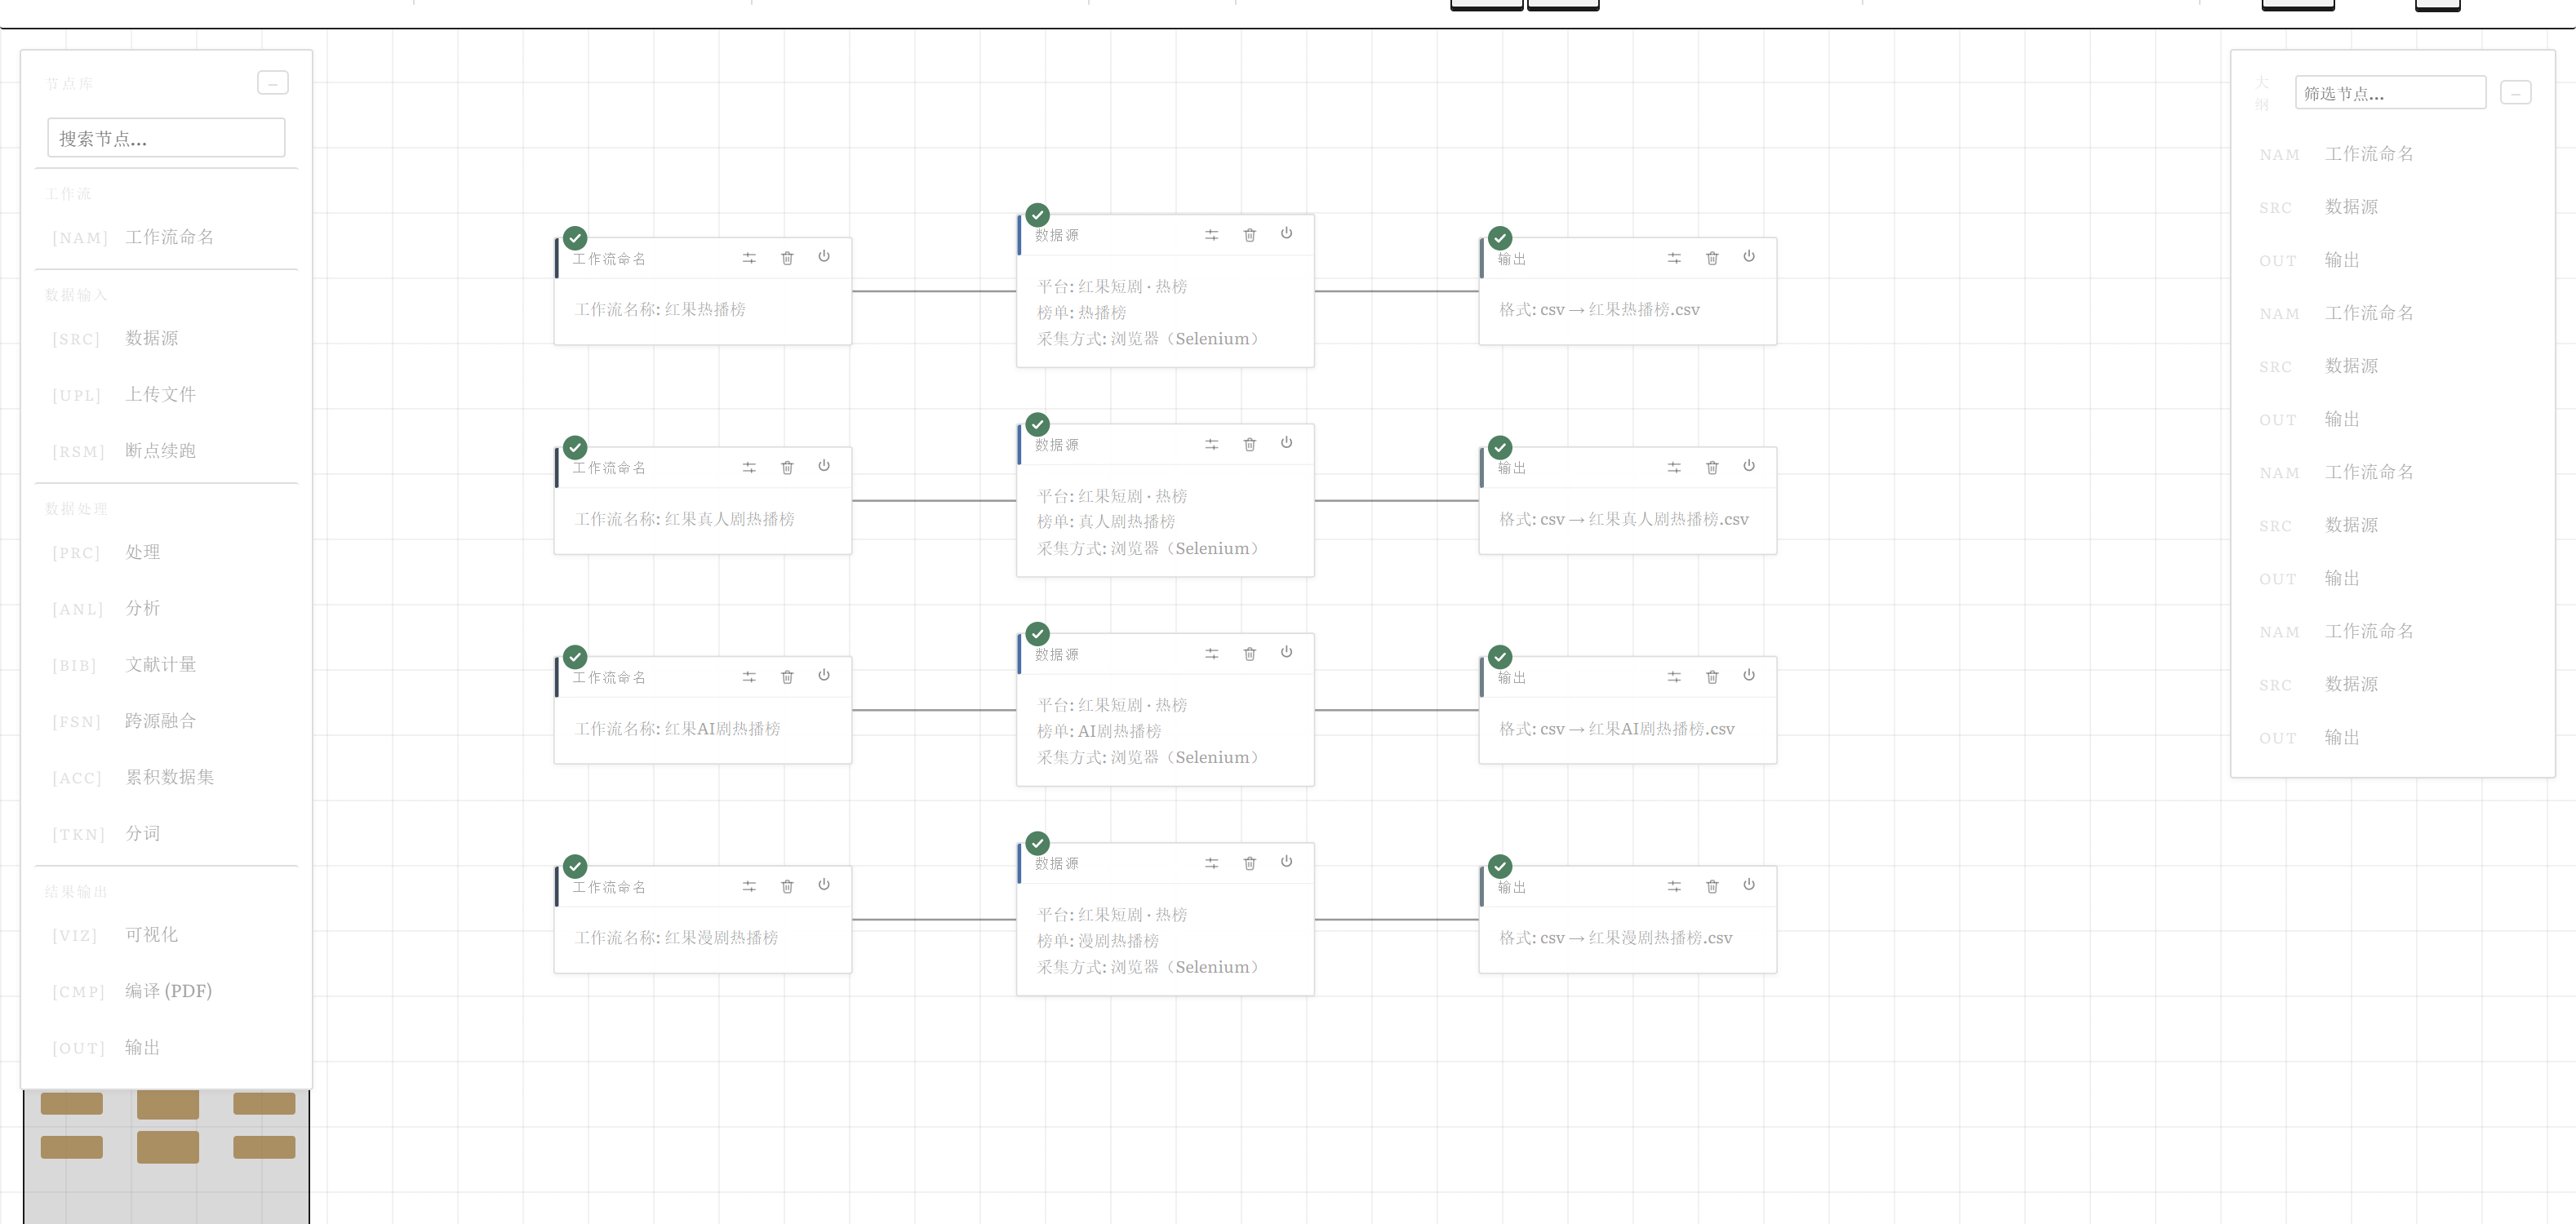
\includegraphics[width=0.98\textwidth]{hg-canvas.png}
\caption{四条链并排，可以并行跑}
\label{fig:hg-canvas}
\end{figure}

\subsection{运行}

菜单条按下“\texttt{并行}”，第一次调试可以不按“\texttt{无头}”，方便看浏览器点了哪里。点“\texttt{执行}”，
控制台先写发现四条工作流，然后四条链交错输出，每条链写每页采了多少条、累计多少、第几页是最后一页。

\begin{figure}[H]\centering
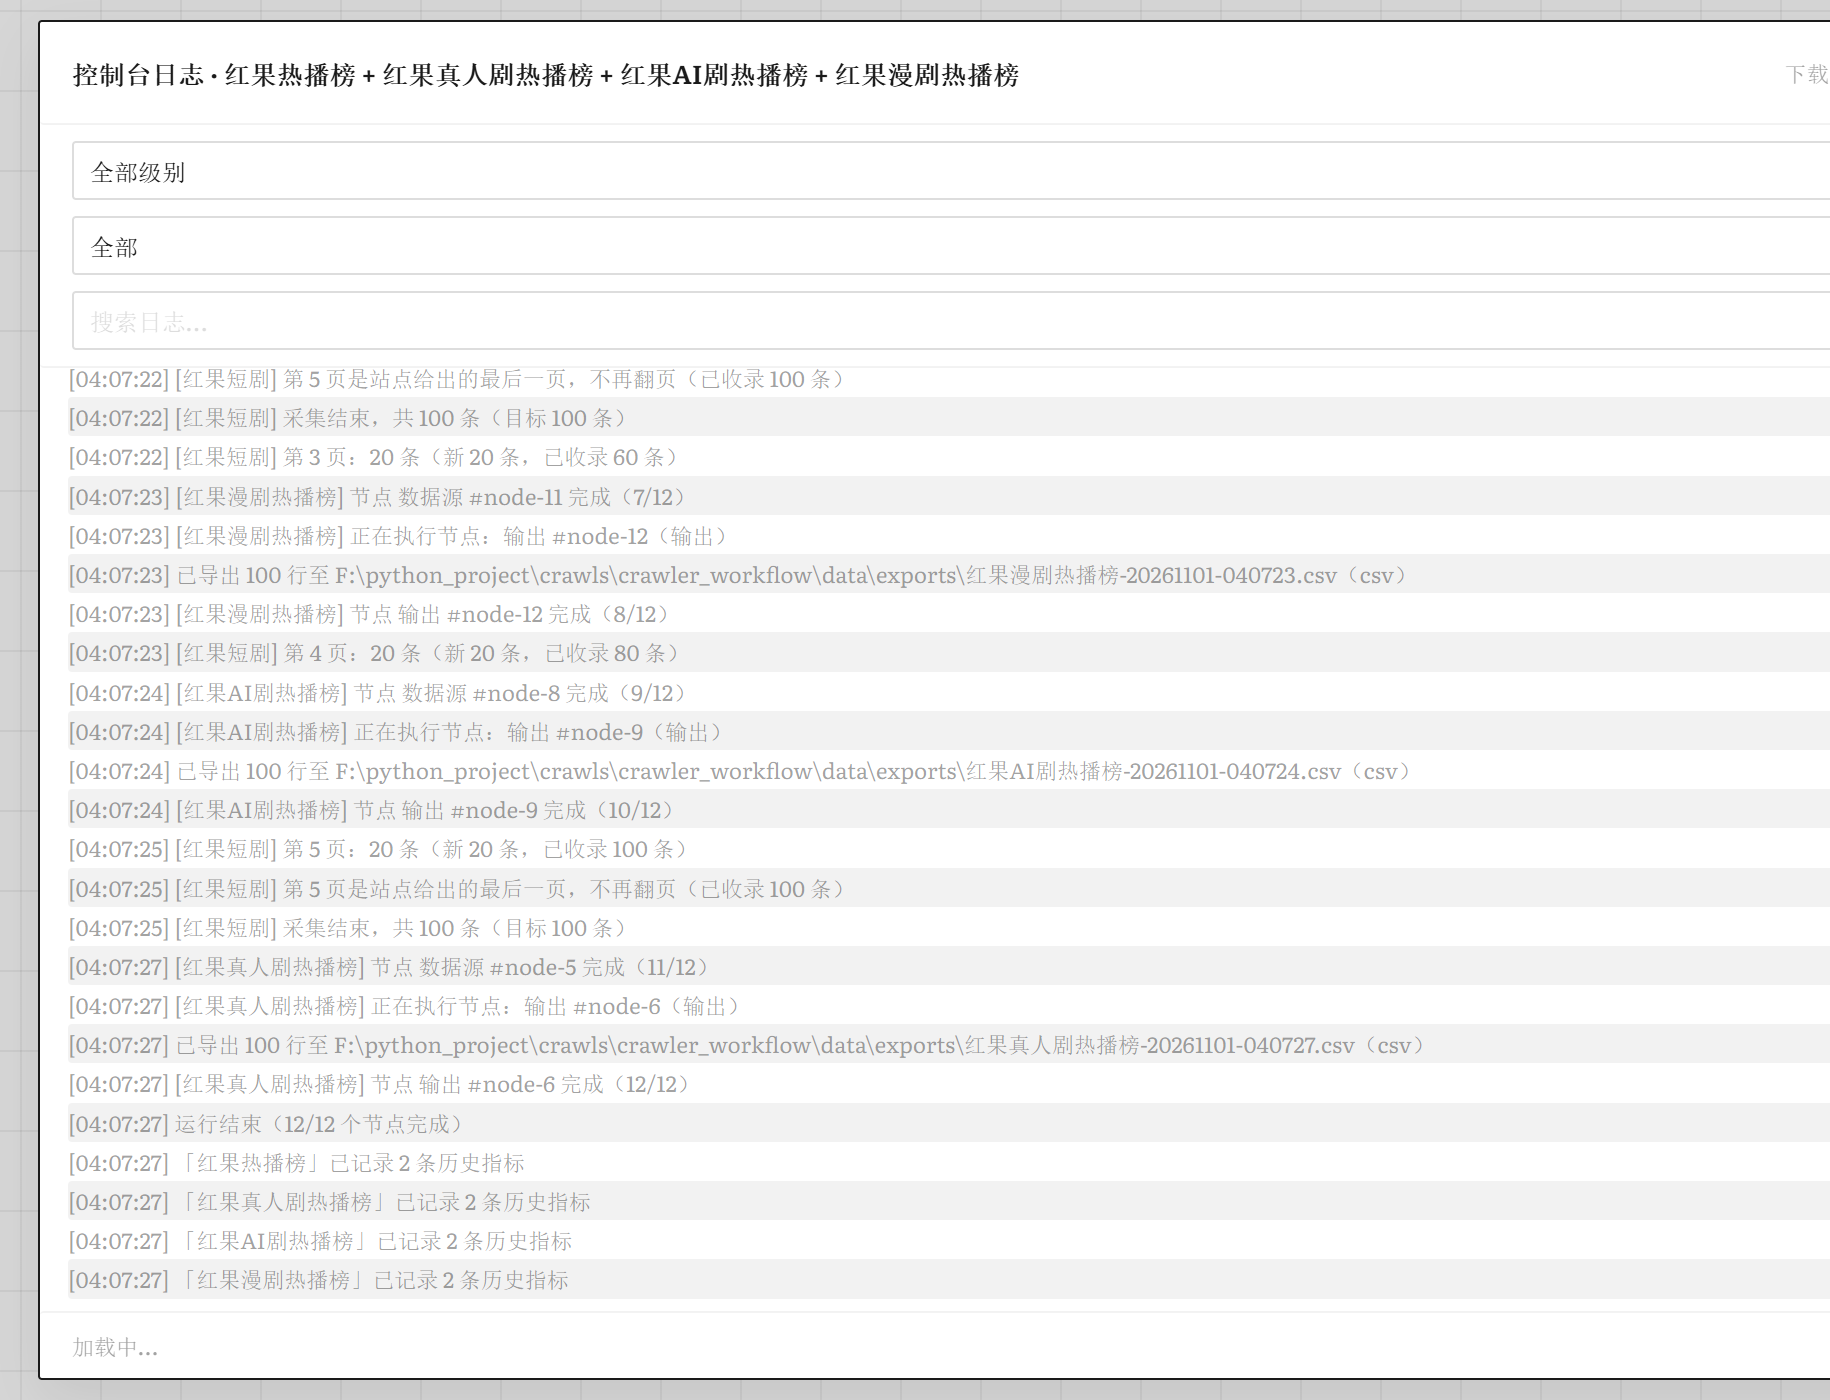
\includegraphics[width=0.94\textwidth]{run-log.png}
\caption{一次运行的完整日志，四条链交错输出}
\label{fig:hg-log}
\end{figure}

两句值得学会看：“\texttt{第 5 页是站点给出的最后一页，不再翻页（已收录 100 条）}”是站点自己的边界；
“\texttt{采集结束，共 100 条（目标 100 条）}”是这条链的结论。两句都在，就是完整结束。

\subsection{看结果}

跑完节点角标变成绿勾。数据源设置底部点“\texttt{预览数据}”，能看到这次真实落下的行：一百行十四列，
列里有作品编号、作品名、评分、热度、分类、标签。这些列名就是下游能用的列名。

\begin{figure}[H]\centering
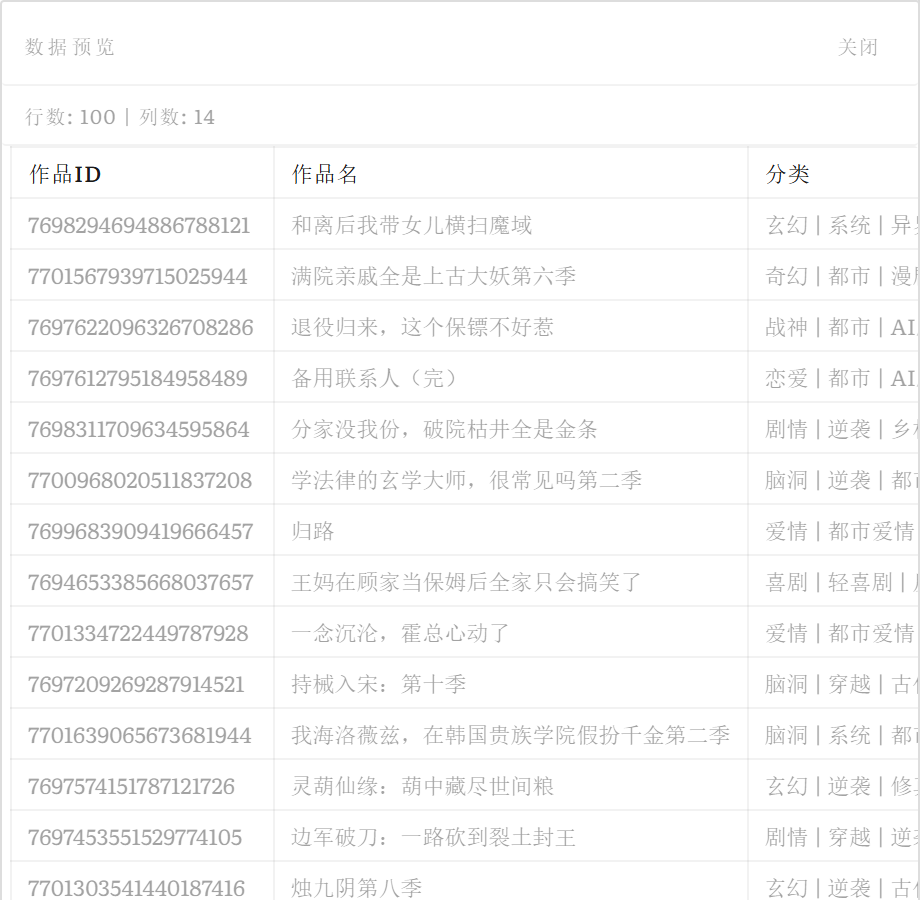
\includegraphics[width=0.9\textwidth]{hg-data.png}
\caption{预览数据：一百行十四列}
\label{fig:hg-data}
\end{figure}

底部“\texttt{导出产物}”里四份 CSV 都在，带运行时间戳，大小接近，时间挨着。点“\texttt{下载}”存到本地。

\section{实战二\quad 热榜转评论}

光有榜单没有内容。这一段把榜单当任务清单，让程序拿着每部剧的名字去抓评论。
仓库里的“\texttt{红果短剧-热榜转评论}”就是这个做法，它比上一节多一个关键动作：上游喂链接。

底部点“\texttt{工作流文件}”，找到“\texttt{红果短剧-热榜转评论}”点“\texttt{打开}”。画布上是两条链，上面一条启用，下面一条关掉。

\begin{figure}[H]\centering
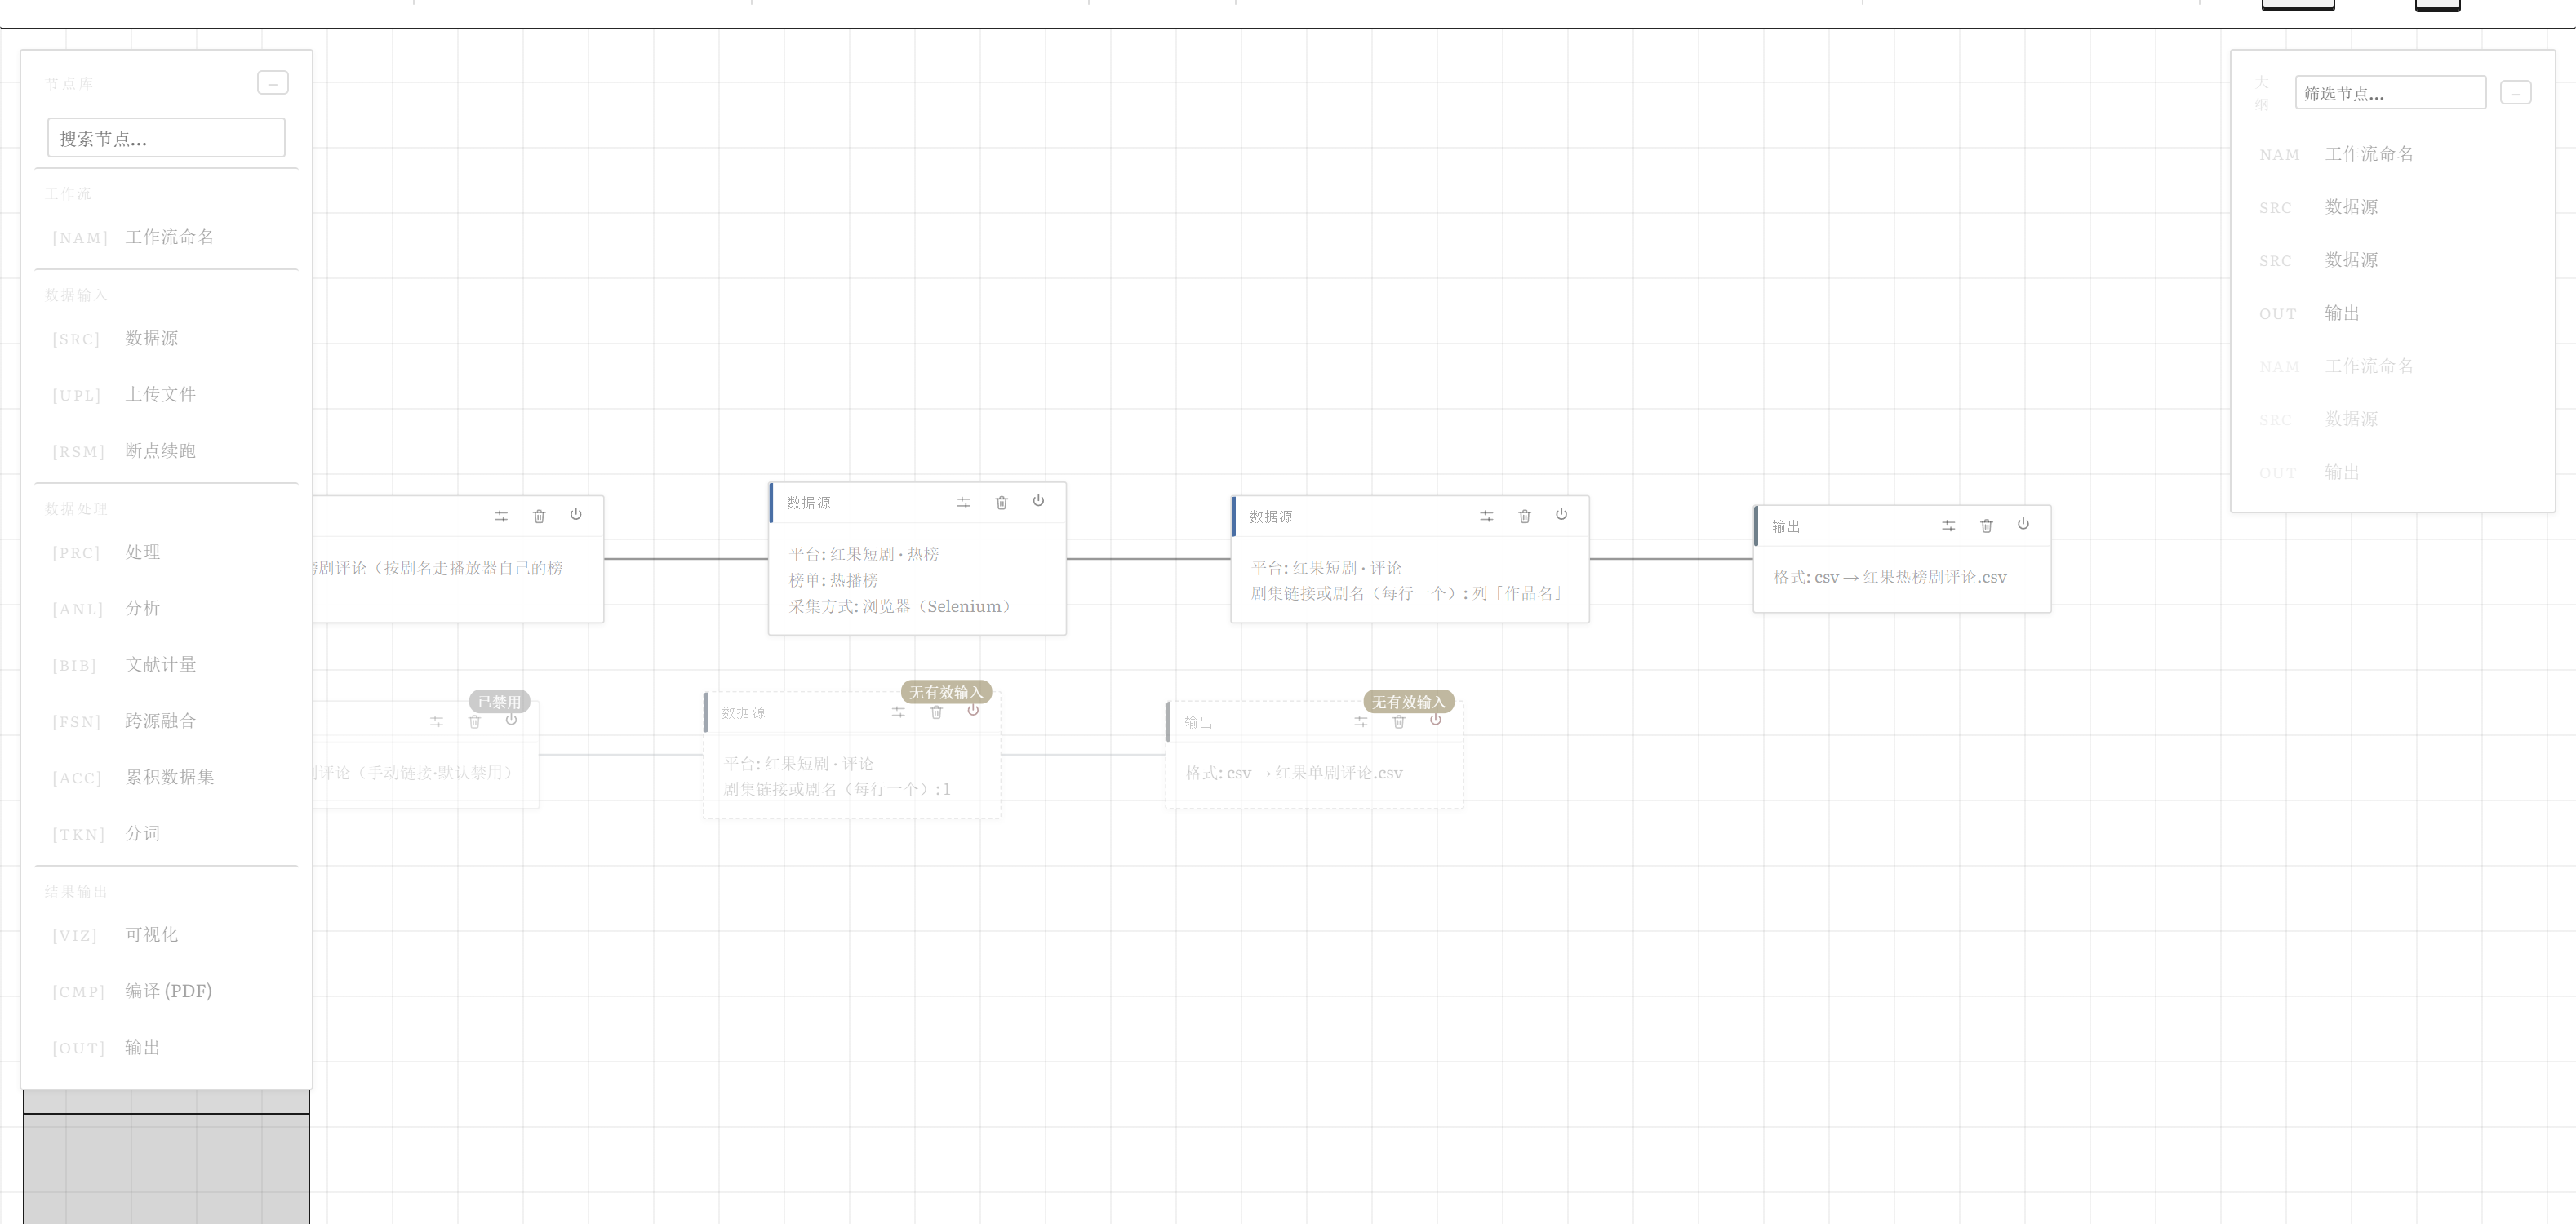
\includegraphics[width=0.98\textwidth]{hg-talk-canvas.png}
\caption{热榜转评论：上面一条启用，下面一条是手动链接的备用链}
\label{fig:hg-talk-canvas}
\end{figure}

上面第一条是命名，第二条采热播榜前十条，与实战一相同，只是数量从一百改成十。第三条才是重点：采集内容选“\texttt{评论}”，
面板里填“\texttt{每部剧集数}”5、“\texttt{包含回复}”打勾、“\texttt{收听超时}”90 秒、“\texttt{每篇单独文件}”打勾、
“\texttt{评论条数上限}”0、“\texttt{评论时间筛选}”留空，最后在“\texttt{上游列名}”填“\texttt{作品名}”。
这一栏就是上游喂任务的开关，填了它，程序逐行取这一列的片名去搜。

\begin{figure}[H]\centering
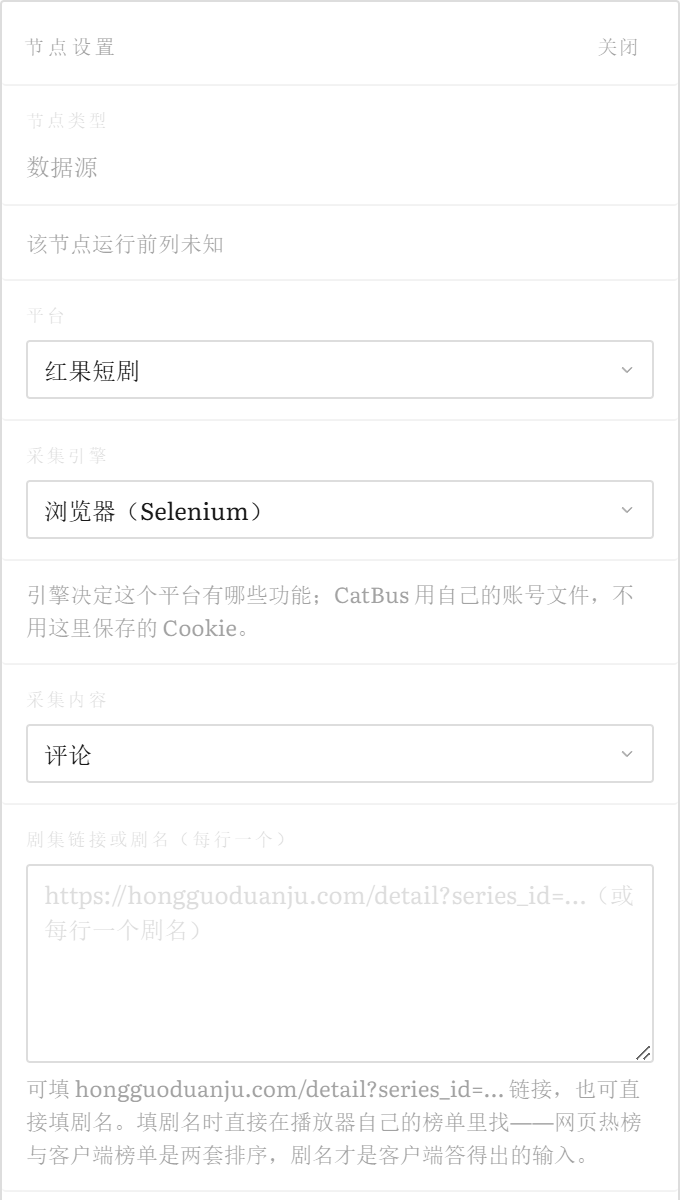
\includegraphics[width=0.31\textwidth]{hg-talk-source.png}
\caption{评论节点的上游列名填作品名，程序拿每一行的片名去搜}
\label{fig:hg-talk-source}
\end{figure}

下面那条链是手动模式，只有一个链接，写在“\texttt{文章链接}”里。命名节点被关掉，所以整条链都不跑，留着当模板：
临时想抓某一部剧，打开它换链接即可。关掉一个节点不会删掉下游，但下游会因为没有输入而一起失效，画布上是灰的，运行时真的不存在。

点执行。上面那条链先拿十条榜单，再拿每一条的剧名去驱动播放器，一条一条听，日志按剧名分组，
写听到了几集、多少条评论、存到哪个文件。红果评论不是从网页读的，程序旁听桌面播放器的通信，所以这台机器要能打开播放器。

这一节练的是两种数据流：一种从站点直接采，另一种拿上游的表当任务清单。后者可以推广到很多地方，
比如拿一份文献清单批量补摘要，拿一份博主清单批量抓主页。

\section{微博的四种采集}

微博把四种采集都做全了，用它能讲清同一个数据源节点的四种形态。打开“\texttt{测试：微博}”，画布上是四条并排的链，加一条关掉的备用链。

\begin{figure}[H]\centering
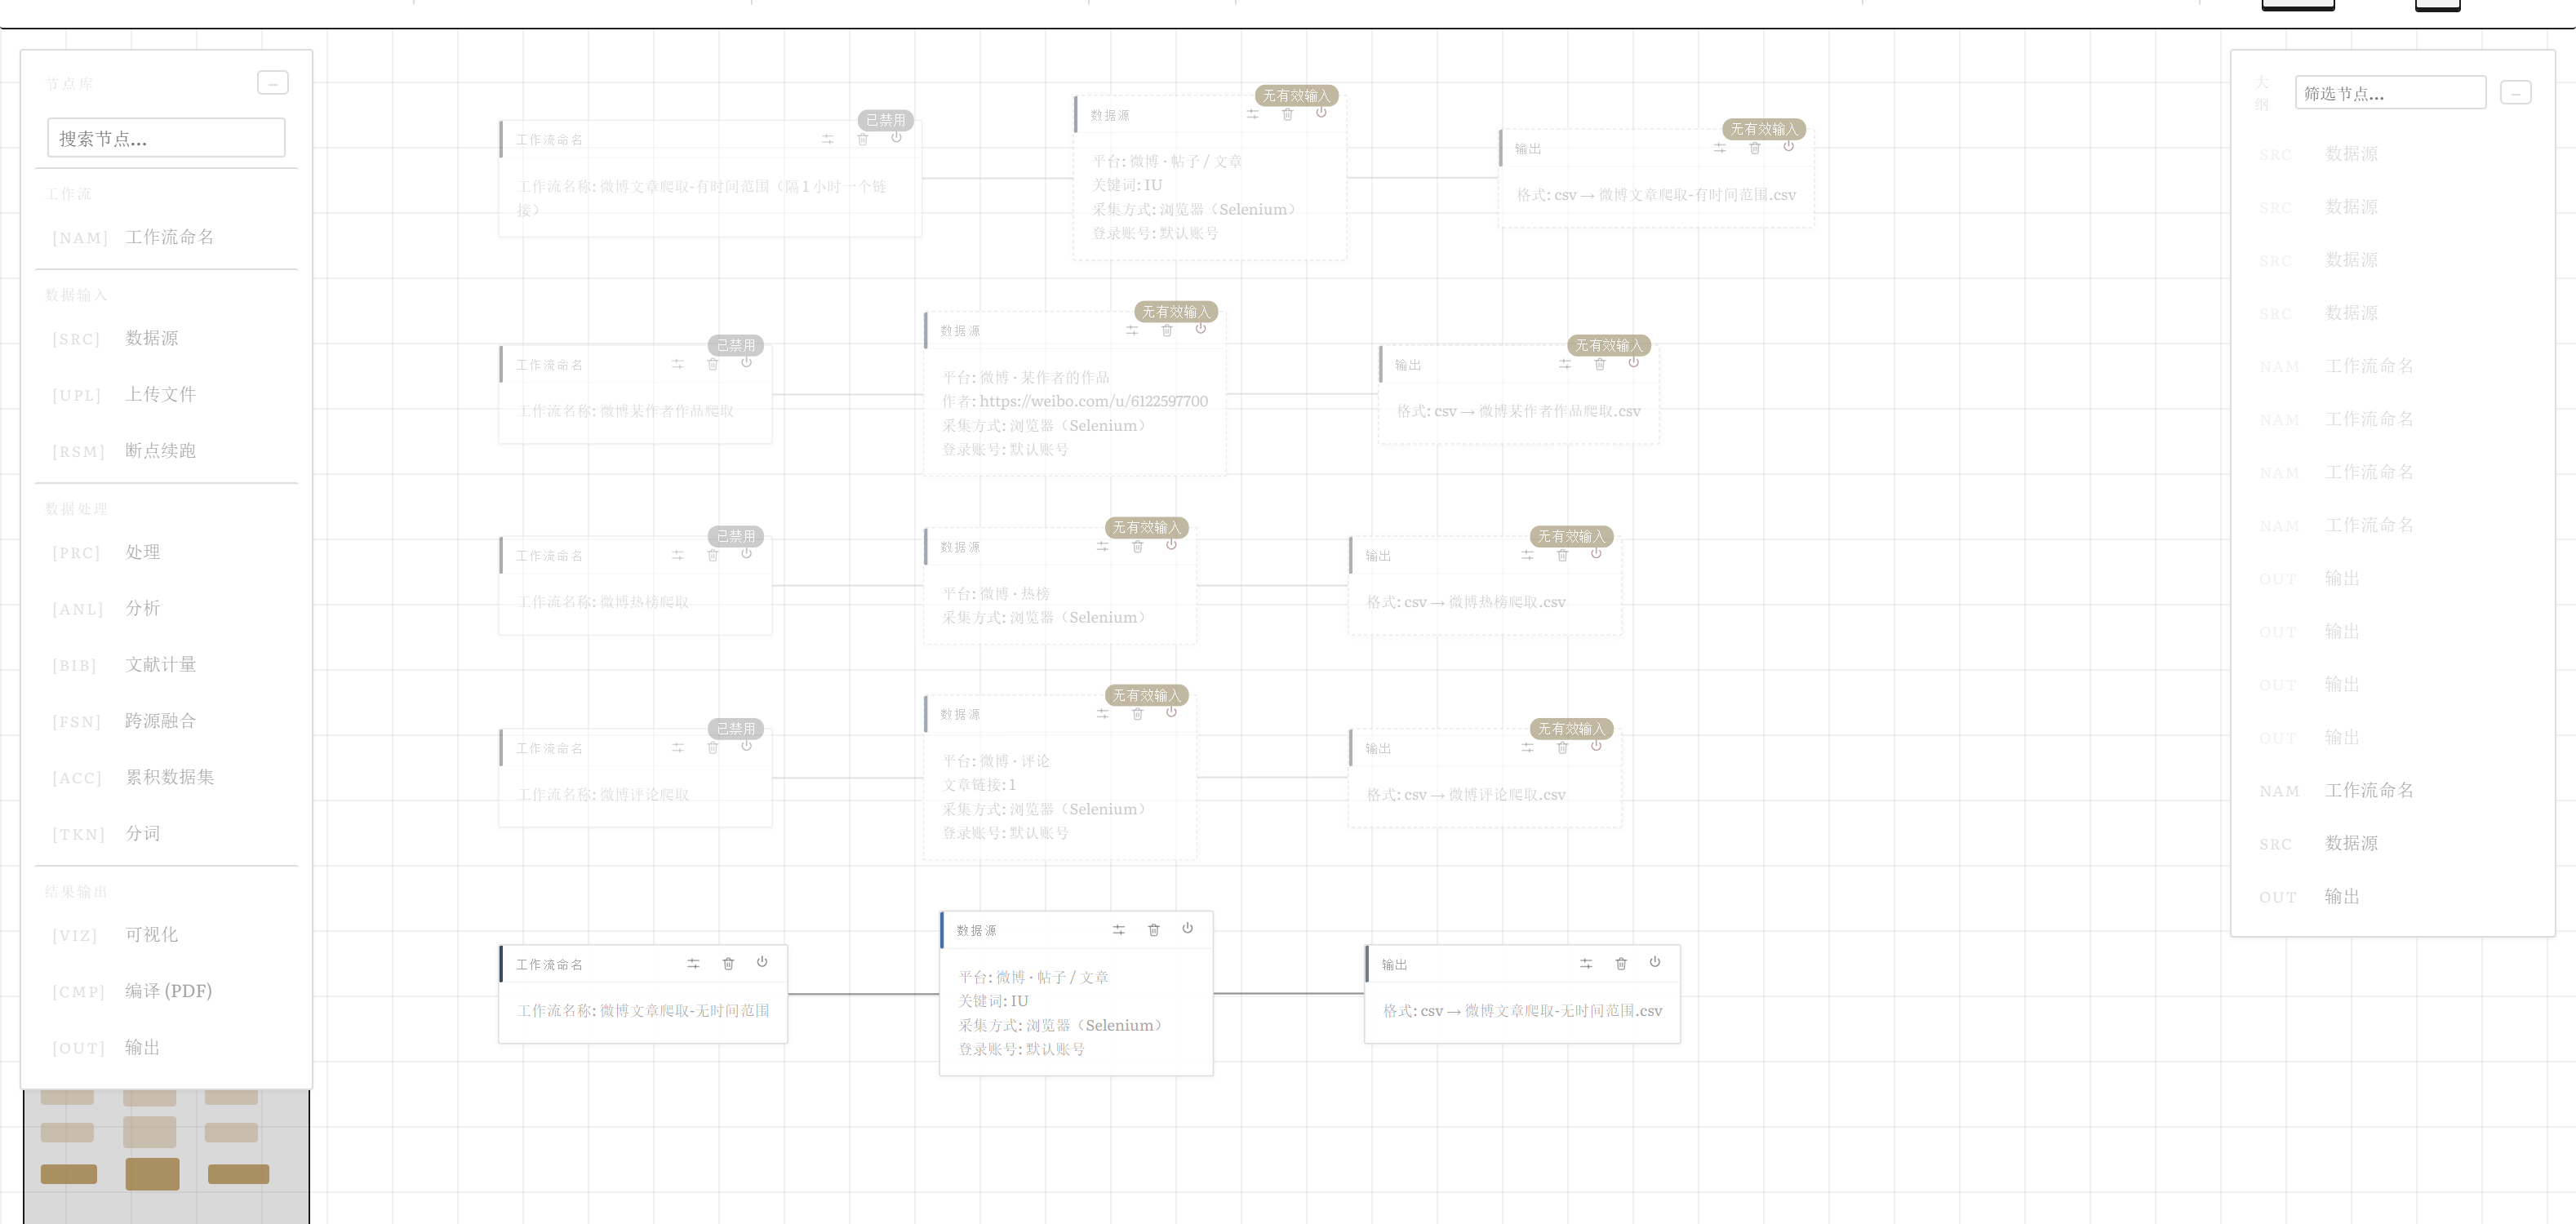
\includegraphics[width=0.9\textwidth]{wb-canvas.png}
\caption{微博四条链：关键词、作者、热搜、评论}
\label{fig:wb-canvas}
\end{figure}

\subsection{关键词与时间范围}

第一条链按关键词采。平台“\texttt{微博}”，内容“\texttt{帖子}”，关键词填 \texttt{IU}，
开始时间 \texttt{2026-01-01}，结束时间 \texttt{2026-09-26}，展开全文打勾，目标数量 50。
微博按时间窗翻页，填了两端就只在这个区间里走。展开全文会点进每条取正文，慢但完整。

\begin{figure}[H]\centering
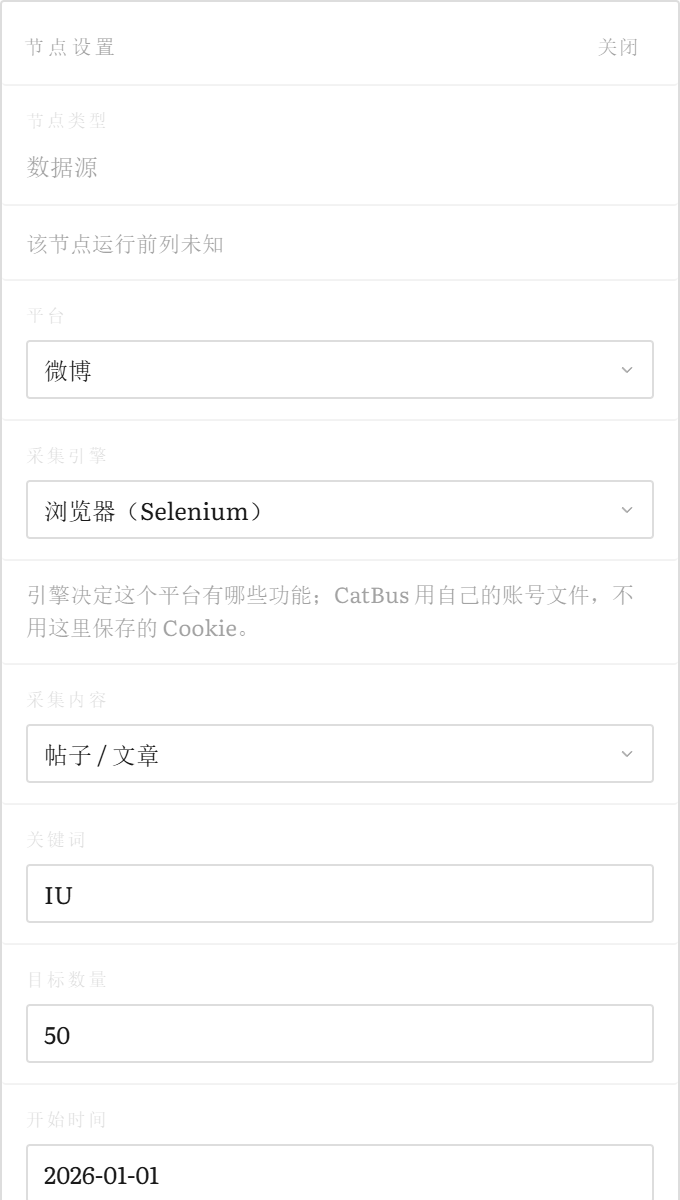
\includegraphics[width=0.31\textwidth]{wb-keyword.png}
\caption{关键词模式：时间范围与展开全文}
\label{fig:wb-keyword}
\end{figure}

时间窗有代价，站点翻得越深越慢，数量不用填太大。程序一路翻到站点给不出下一页为止。

\subsection{作者作品}

第二条链把内容换成“\texttt{某作者的作品}”，作者填主页链接或者那串数字 UID。作者这一栏要么填完整链接，要么填纯数字，
填昵称不行，填错时程序会拒绝并说明要哪种形式。作品列表从作者主页自己的接口一页页取，不需要登录也能看到公开部分。

\subsection{热搜}

第三条链选“\texttt{热搜}”。这一项不需要登录，采到的是当下这一刻的榜单，带精确整数热度。
即时榜重复运行会把同一时刻的榜再存一遍，要不要重采看用途。

\subsection{评论}

第四条链采评论，文章链接写一条微博地址，每篇单独文件打勾。评论节点与别的平台共用一套面板：
能设评论时间筛选、是否包含回复、条数上限，上游是表时还能按某一列逐行喂链接。

\begin{figure}[H]\centering
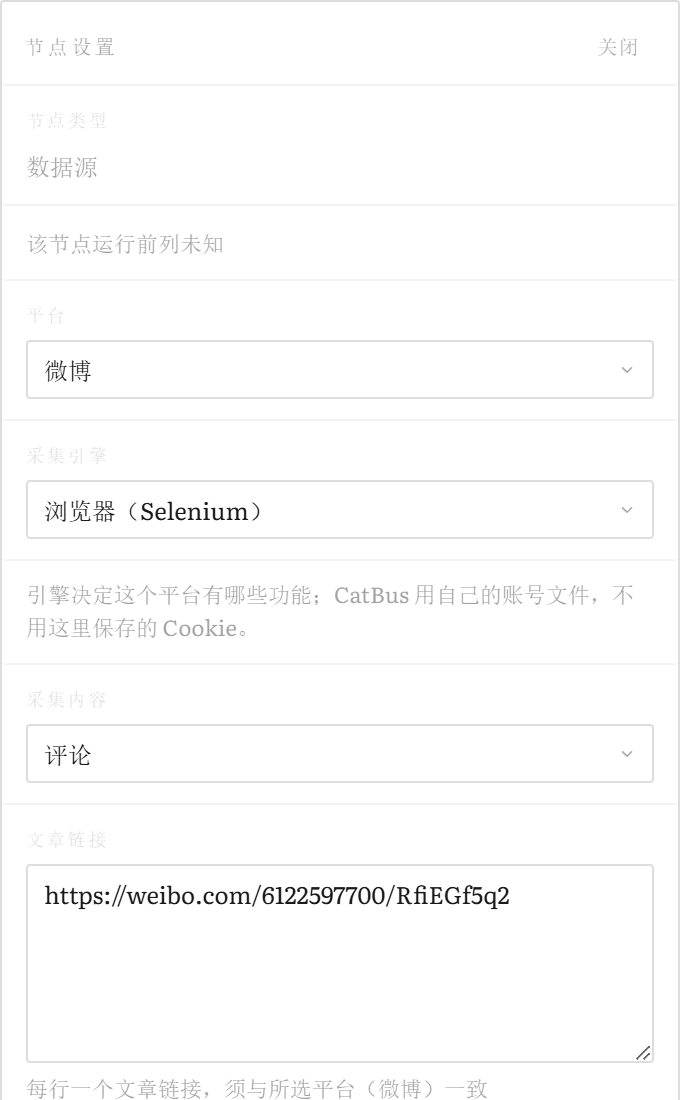
\includegraphics[width=0.31\textwidth]{wb-comment.png}
\caption{评论节点：时间筛选与条数上限}
\label{fig:wb-comment}
\end{figure}

有些平台、有些视频不发布评论者的 IP 属地，评论地区这一列可能是空的。画布里只要出现评论节点，运行前会提示一次，纯搜索的画布不会打扰。

\section{抖音作者、评论与两路分析}

这一条链把采集和模型接在一起。打开“\texttt{测试：抖音}”。三段：作者作品、评论、两路情感分析。

\begin{figure}[H]\centering
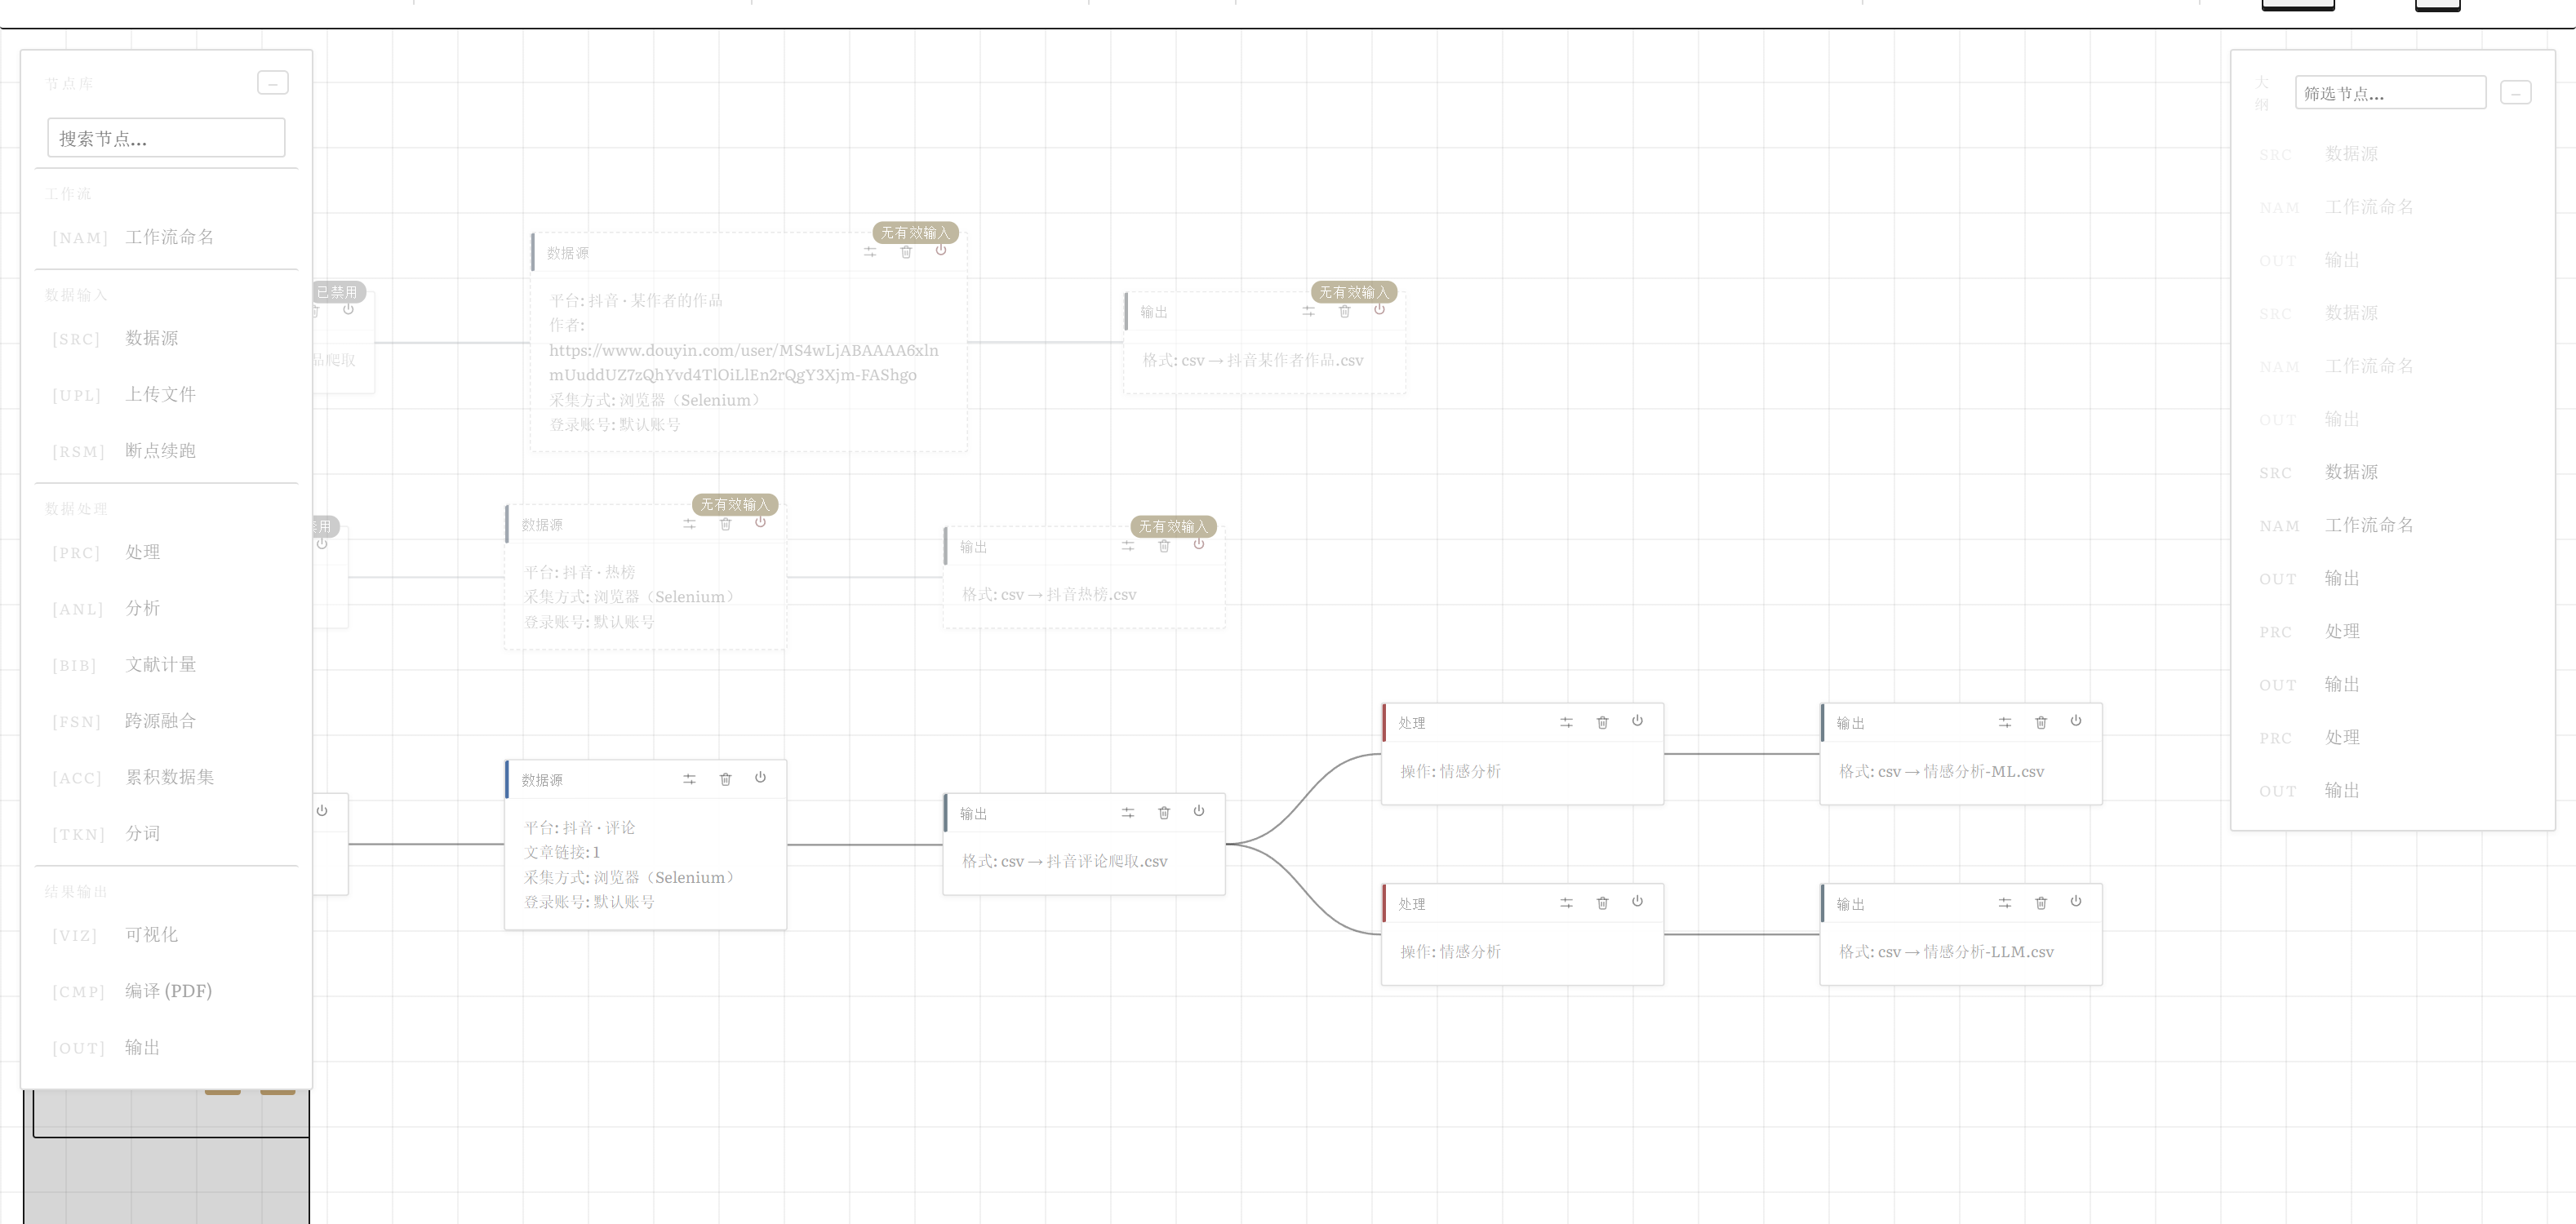
\includegraphics[width=0.98\textwidth]{dy-canvas.png}
\caption{抖音三段：作者作品、评论、两路情感分析}
\label{fig:dy-canvas}
\end{figure}

数据源选“\texttt{抖音}”，内容“\texttt{某作者的作品}”，作者填主页链接。抖音只认链接里那串 \texttt{sec\_uid}，填昵称会被拒收。
作品网格在站内用遮罩打开，程序读遮罩里的卡片，不逐条跳转。第二个数据源采评论，链接写一条视频地址，
评论面板要一路滚到底，楼层号按站点给出的顺序编号。

后面两个“\texttt{处理}”节点都是情感分析，用同一个文本列，区别只在分析模式：一路传统机器学习，一路大模型。
一次跑完就能对比两种模式的结论、费用与耗时。

\begin{figure}[H]\centering
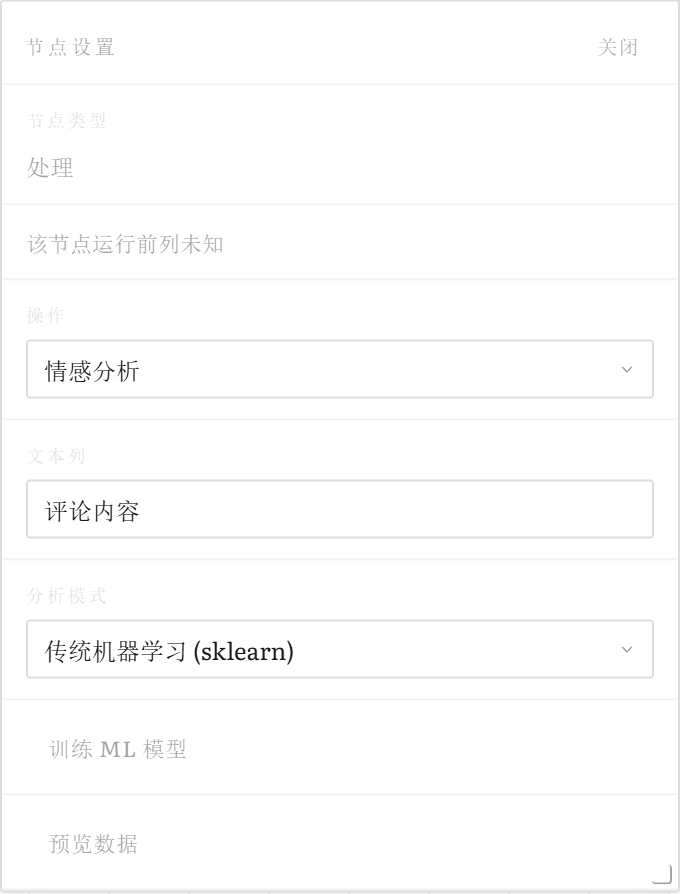
\includegraphics[width=0.31\textwidth]{dy-sentiment.png}
\caption{情感分析节点：操作、文本列、分析模式三行必填}
\label{fig:dy-sentiment}
\end{figure}

BERT 跑不起来时节点自动降级到机器学习，并在控制台写明这一轮实际用的是哪种，不会把降级结果说成 BERT。
大模型那一路逐行调用，日志里能看到每批保存了多少行。跑完两个输出文件分别是“\texttt{情感分析-ML.csv}”与“\texttt{情感分析-LLM.csv}”，
同一批评论两套结论，可以直接拿去做对比图。

\section{知乎关键词到词云}

这一条最短，覆盖采集到出图的全程。打开“\texttt{测试：图表可视化}”。

\begin{figure}[H]\centering
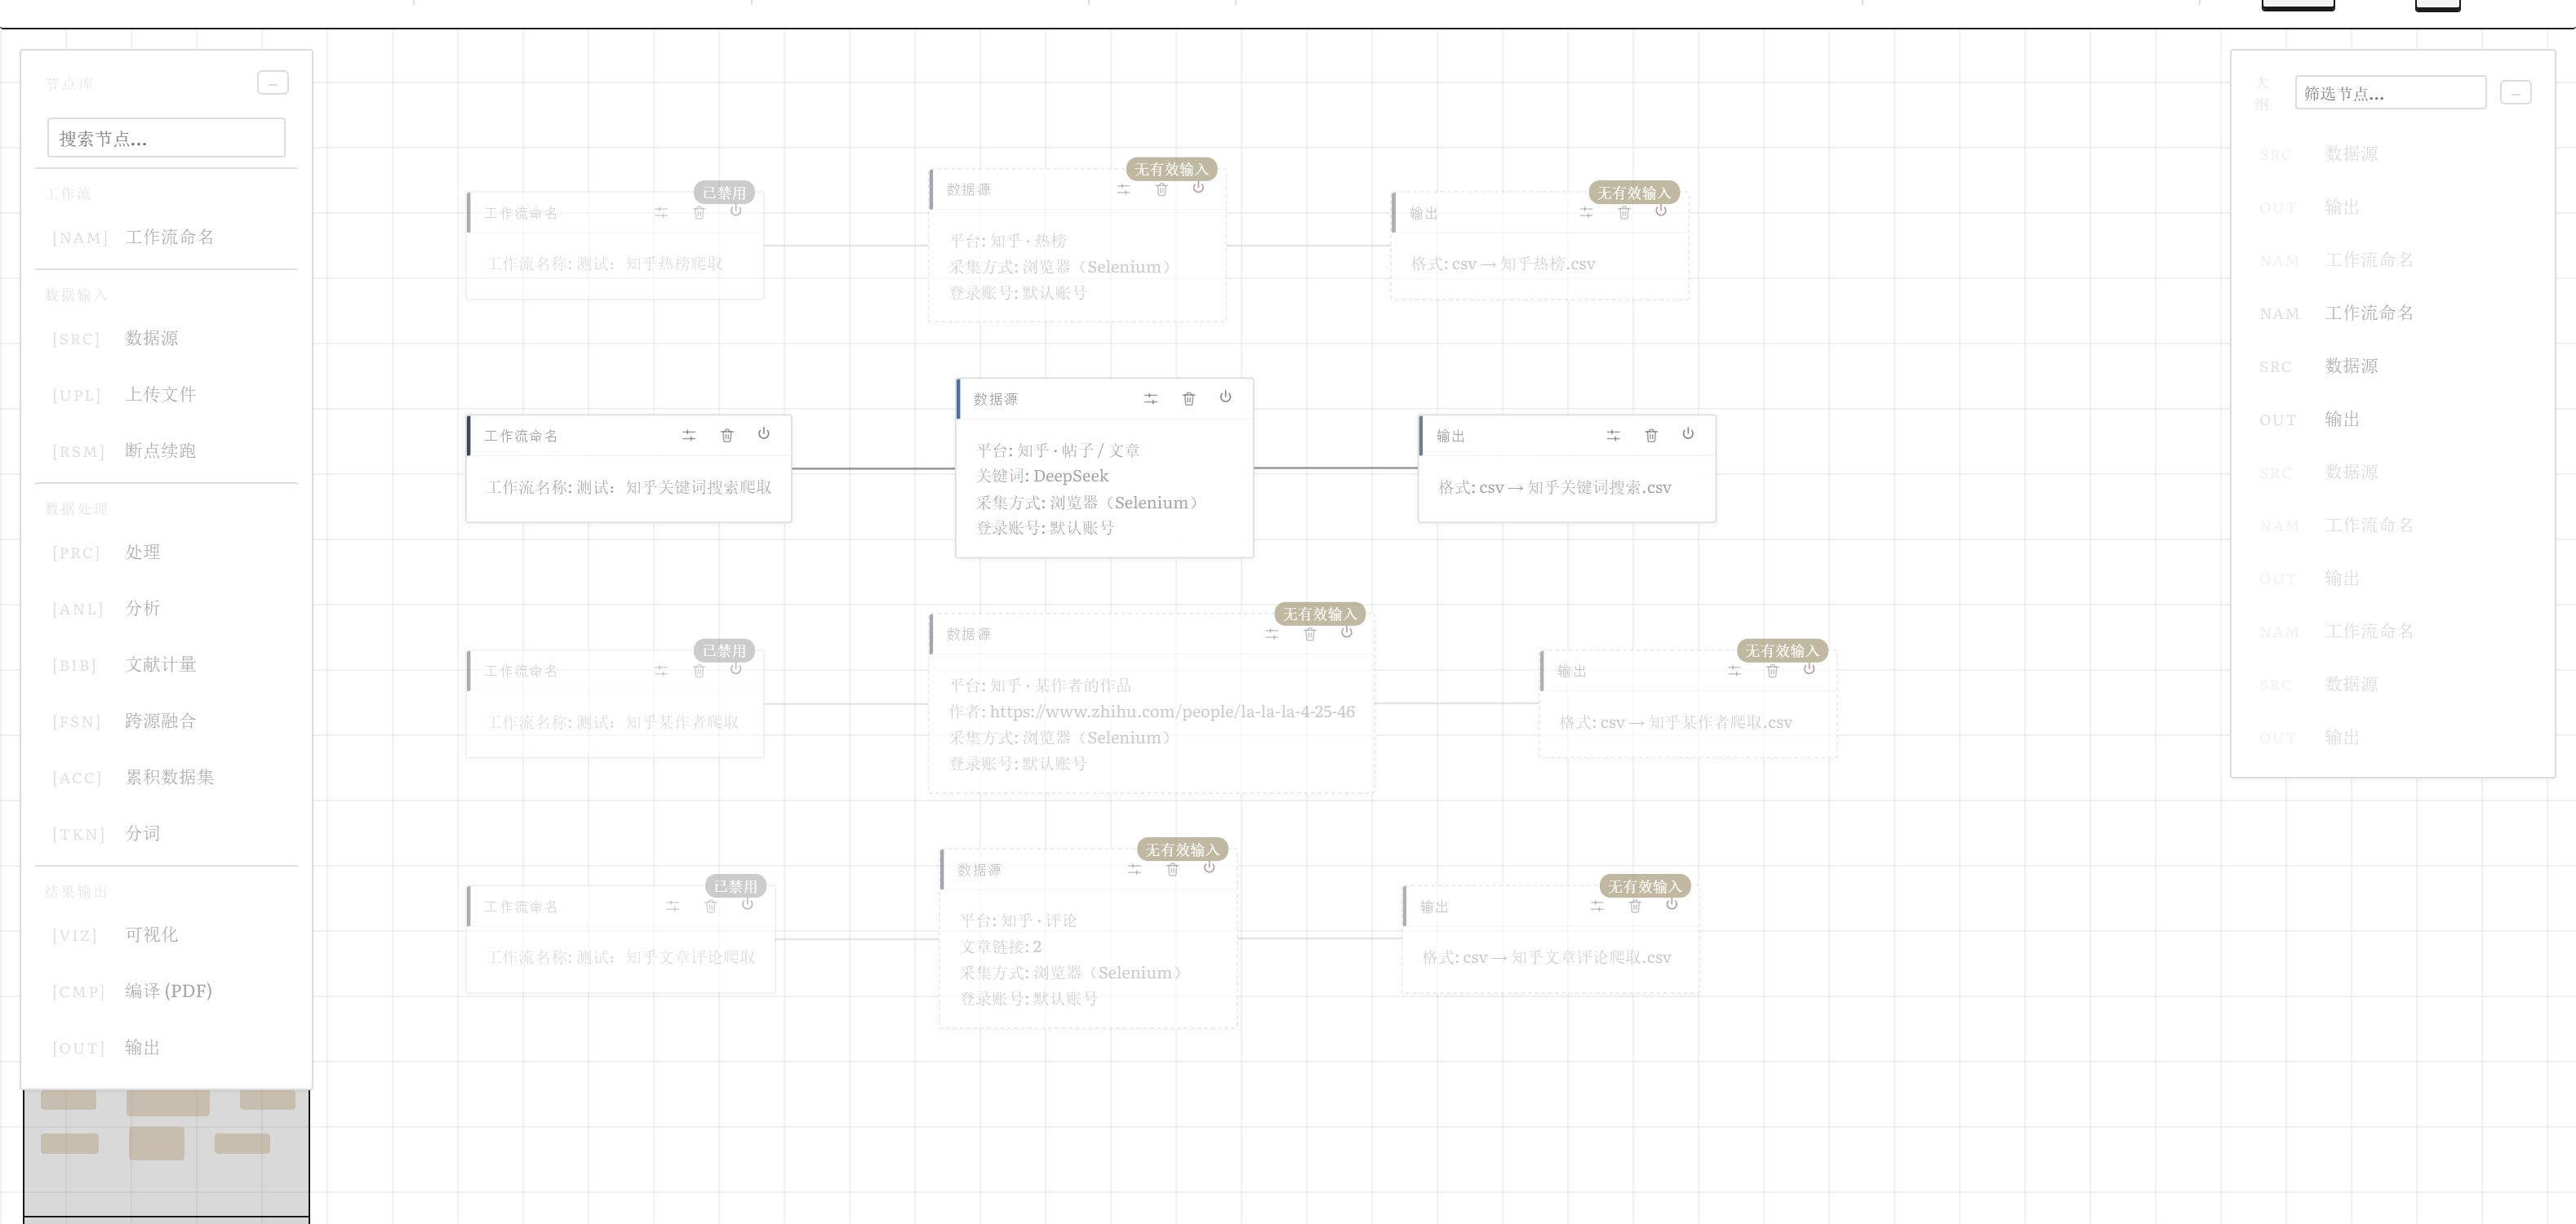
\includegraphics[width=0.98\textwidth]{zh-canvas.png}
\caption{知乎关键词采下来，改列名，出一张词云}
\label{fig:zh-canvas}
\end{figure}

数据源选“\texttt{知乎}”，内容“\texttt{帖子与文章}”，关键词“\texttt{世界杯}”，目标 20 条，展开全文打勾。
知乎搜索卡片只给摘要，勾了才会把全文读进来。

中间“\texttt{分析}”节点的操作是“\texttt{重命名列}”，把“\texttt{作者}”改成“\texttt{发帖人}”。上游列名不合适，
或者下游要按固定列名读，就在这里改一次，后面全部统一。

最后一个“\texttt{可视化}”节点，图表类型“\texttt{词云}”，引擎 \texttt{ECharts}，横轴字段“\texttt{正文}”，分词打勾。
词云直接吃原文，自己切词，不必先过“处理 → 分词”。

\begin{figure}[H]\centering
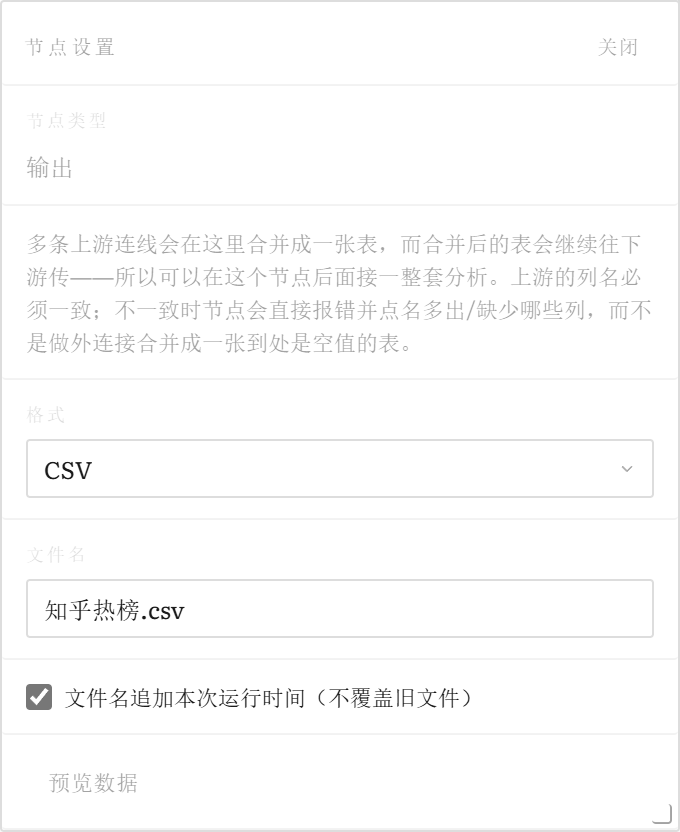
\includegraphics[width=0.31\textwidth]{zh-visualize.png}
\caption{可视化节点：图表类型、引擎、LaTeX 选项、标题}
\label{fig:zh-visualize}
\end{figure}

面板底部三个按钮：预览图表看效果，预览数据看这张图的输入表，图表工坊把这份数据送进作图台。跑过一次以后才有内容可看。

\section{采集疑难}

问题大多出在登录、速度、并发三件事上。

\subsection{登录过期}

症状是跑到一半跳到登录页，日志写登录墙。打开“\texttt{Cookies}”，选平台与账号，重新存一份再验证。
已经采到的行不会丢，重新执行会从断点接上。微博有一种假登录墙，搜索时页面会闪一下扫码页再弹回结果，
程序等页面稳定再判断，真掉线才报错。

\subsection{同一平台并行}

同一份浏览器目录同一时刻只能开一个。画布上有两条以上同平台的链又勾了并行，运行前会问你一次：
排队跑、换账号或者串行。设置里“\texttt{同平台排队采集}”打开就是真排队，一次只跑一条，前一条完才轮到下一条；
“\texttt{同平台错峰间隔}”给不排队的情况留一个几秒的缓冲。

\subsection{采得慢或者采不到}

站点风控会限制频率。设置里的“\texttt{慢速采集}”打开以后每轮操作之间多停一会儿，不是万能，但比硬撞好。
海外平台还要网络通。画布上出现海外平台时，运行前会问一句外网通不通，不通先挂上再跑，别把超时当站点改版。

\subsection{采到的行数不够}

看日志最后一句。写的是站点给出的最后一页，就是真到底了；写的是风控、登录、超时，就是被拦住了。
换时间、换账号、开慢速再试。程序不会把短表默默交给你，一定说明为什么短。

\subsection{第二套采集后端}

有些平台只能用 CatBus，比如快手、TikTok、京东、淘宝、闲鱼，这类平台的采集引擎下拉里只有它。
CatBus 要本机装 Node 与它的适配器，缺哪一样都按名字说清是缺哪一样，不会给一张空表然后标成完成。
它的登录门与浏览器那套分开，用自己的账号文件，登录状态也不与 Cookie 面板混用。

\section{上传与数据集}

不采集也能用。手上有表格时，第一个节点用“\texttt{上传文件}”。

\begin{figure}[H]\centering
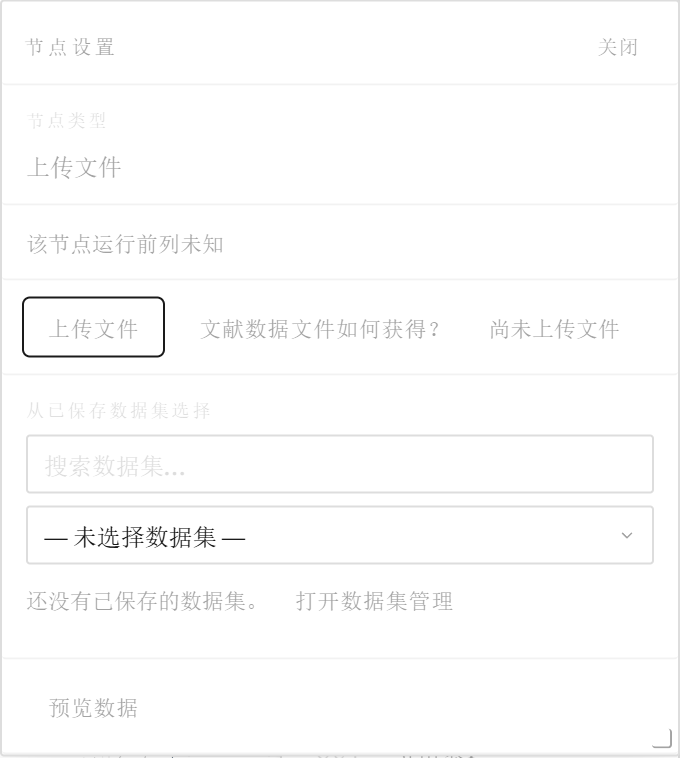
\includegraphics[width=0.31\textwidth]{panel-upload.png}
\caption{上传节点：从文件选，或挂一份已存数据集}
\label{fig:panel-upload}
\end{figure}

\subsection{支持的文件}

CSV、TSV、JSON、TXT、Excel 是最常用的五种。文献工具导出的 NBIB、RIS、BibTeX、EndNote、NoteExpress 也能直接读，
程序把它认成文献记录表，不需要先整理列名。

Excel 一次只读一张工作表。一个文件里有好几张非空的表时会拒绝并列出表名，让你先把要的那张单独存出来或转成 CSV。
两张表列不一样，硬合会错位。

\subsection{上传以后发生什么}

文件算一个内容哈希，压进本地库，登记成数据集。以后这份工作流打开时可以直接挂回这份数据，不用再找原文件；
同一份文件重复上传不会存两份，认的是哈希。

“\texttt{数据集}”面板能看到每份文件的来源、列数、行数、被哪些工作流引用，可以改名、删除、合并。
被工作流引用的数据集单独删会当场拒绝，面板顶部的清空是例外，它连被引用的也一起删，确认框里写清了这个区别。

\begin{figure}[H]\centering

\includegraphics[width=0.43\textwidth]{datasets.png}
\caption{数据集面板，一份表格一行}
\label{fig:datasets2}
\end{figure}

上传面板里还有一条捷径，从已保存的数据集里选，适合反复用同一份底表做不同的分析。

\subsection{合并同构的数据集}

两份表列一样时，数据集面板能把它们合并成一份，默认加一列来源记下每一行来自哪份。
列多了少了都会按名字拒绝，并告诉你是哪一列对不上。

\section{清洗}

采集回来的文本很脏：转发链、提及、话题标记、链接、表情代码混在一起，还有水军刷的重复稿。
清洗节点干两件事，剥掉噪音，判断这一行跟主题有没有关系。

“\texttt{正则}”模式不花模型的钱，规则固定。它剥掉转发链只留你自己那段，去掉提及、话题标记、链接与表情代码，
整行只剩这些东西的判为删除。原文保留，清洗结果写在 \texttt{cleaned\_text} 列。
“\texttt{模型}”模式逐行问一次模型，判断内容是否与主题相关，顺便过滤广告与灌水，更聪明也更慢，几千行以上要算清成本。

\section{去重}

去重不是一个算子，是三个，按粗到细排。

\begin{figure}[H]\centering
\begin{tikzpicture}[node distance=6mm]
  \node[card=src,text width=2.5cm] (raw) {原始行\\[2pt]\micro 3000 条};
  \node[card=prc,right=of raw,text width=2.7cm] (exact) {逐字去重\\[2pt]\micro 完全相同才删};
  \node[card=anl,right=of exact,text width=2.7cm] (norm) {归一化去重\\[2pt]\micro 忽略链接与标记};
  \node[card=viz,right=of norm,text width=2.7cm] (sim) {近重复去重\\[2pt]\micro 指纹距离};
  \draw[wire] (raw) -- (exact);
  \draw[wire] (exact) -- (norm);
  \draw[wire] (norm) -- (sim);
  \node[micro,below=5pt of norm] {改写的水军稿在这里被抓到};
  \node[micro,below=5pt of sim] {改一个词的转发在这里被抓到};
\end{tikzpicture}
\caption{三层去重，一层比一层松}
\label{fig:dedupe}
\end{figure}

逐字去重看整行是否完全一样。归一化去重在比较之前先把链接、提及、话题、表情抹平，所以同一句话换个链接发两次也能认出来。
近重复去重用 SimHash 指纹，距离默认八位，抓改了一个词的转发。距离调大召回更高、精确率更低；
微博评论里改一个词大约差五到十八位，两条互不相关的评论差二十六到二十八位，所以八是个合理的起点。

\section{确定性算子}

分析节点里有一批不需要模型的算子，日常清理够用。

\begin{table}[H]\centering
\caption{常用确定性算子}
\label{tab:ops}
\small
\begin{tabularx}{\textwidth}{p{3.2cm}X}
\toprule
算子 & 用途 \\
\midrule
去空值 & 任一列为空即删，或全部为空才删 \\
填充空值 & 填一个值，或者前向、后向填充 \\
条件筛选 & 按一列的值保留行，等于、不等于、包含、为空 \\
选择列 & 只留要的几列，顺序按你写的来 \\
重命名列 & 上游列名不合适时在这里改 \\
去除空白 & 去掉首尾空格，中文全角空格也清 \\
类型转换 & 文本转数字、转日期 \\
排序 & 按一列或多列排，升降序可选 \\
采样 & 随机抽若干行，做小样本试验 \\
分组聚合 & 按一列分组，对另一列求和、均值、计数 \\
表关联 & 两张表按一个键拼起来 \\
列计算 & 两列相加、相除，结果写进新列 \\
数值分箱 & 等宽分箱，或自己给边界与标签 \\
\bottomrule
\end{tabularx}
\end{table}

这些算子出错会直接失败，不给一张空表：给文本列求和、比较条件填了非数字、指定的列不存在，都属于这一类，
报错信息会点名是哪个节点、哪一列。

\section{时间与阶段}

做事件研究要先有阶段。三个算子把时间拆开，各管一段。

“\texttt{提取时间}”从时间列派生新列，可以派生日期、小时、星期、月份。解析不了的相对时间标签留空，程序不猜年份。

“\texttt{按时间划分阶段}”用一串边界给行打阶段标签，规则是左闭右开，边界前一天二十三点五十九分的行还算前一个阶段。
面板里填三样：列选时间列，边界从早到晚写，最后一个边界是最后阶段的次日；阶段名按顺序写，个数比边界少一个。

\begin{figure}[H]\centering
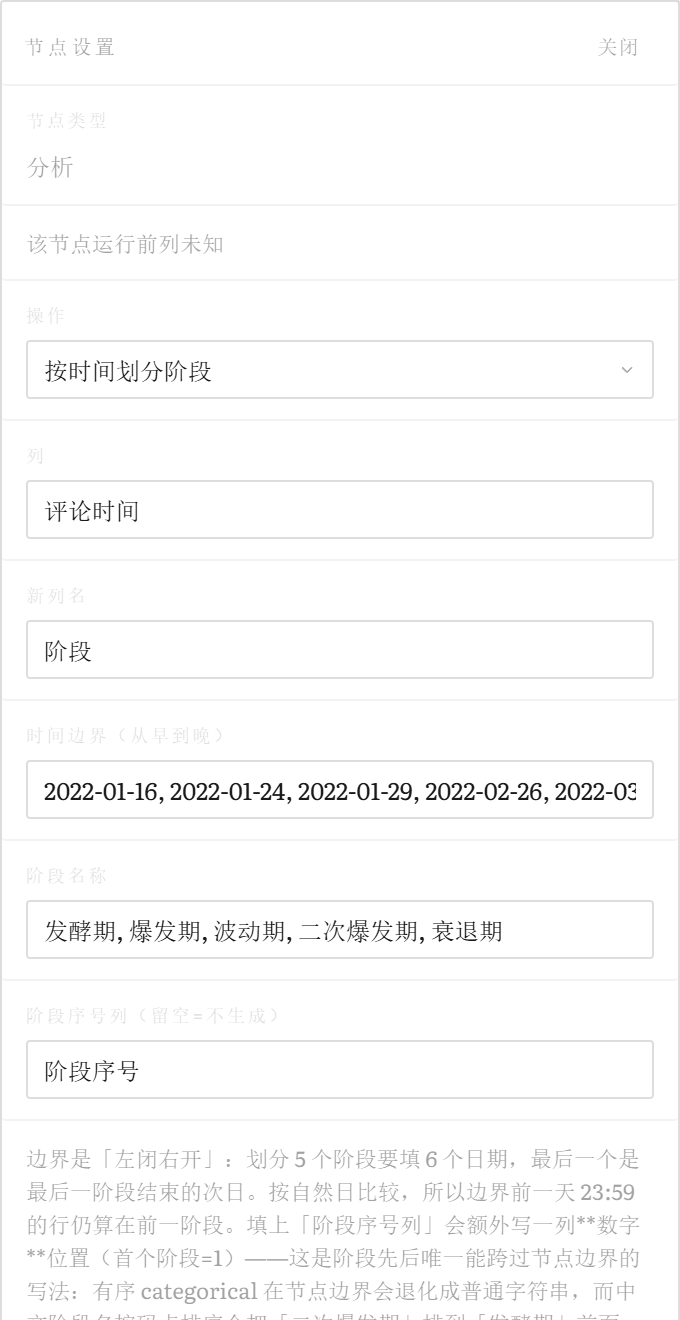
\includegraphics[width=0.31\textwidth]{liu-stage.png}
\caption{划分阶段：六条边界切出五个阶段}
\label{fig:liu-stage}
\end{figure}

“\texttt{阶段序号列}”建议填上。阶段列是有序的类别，但每过一个节点表格会被重建成普通文本，
中文阶段名按字符码排序会把“二次爆发期”排到“发酵期”前面，一张按阶段分组的表就读反了，而它看起来依旧完整。
所以划分阶段会额外写一列数字，第一阶段是一，往后递增。分阶段主题、主题生命周期、主题流向这些要按先后算的步骤读的都是这一列数字，
两个都没有时它们会拒绝，不按名字猜先后。

不知道边界怎么切时，用“\texttt{按发文量建议阶段边界}”。它读每日发文曲线的峰谷，把能直接粘进上一步的边界与标签打印出来。
峰的定义是一段连续若干天高于日常中位数若干倍，太短的窗口会并入行数更多的邻居，并提醒你并了哪一段。

\section{模型接入}

凡是逐行读文字的节点，都要一个模型。模型有两个来源，二选一。

\begin{figure}[H]\centering
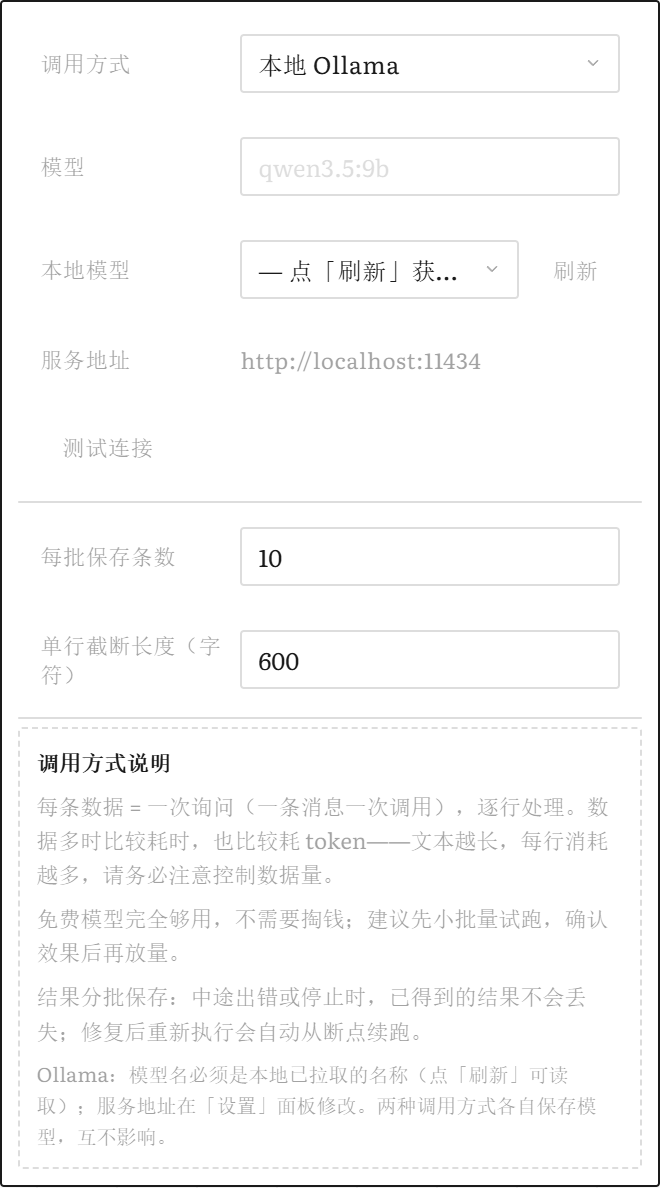
\includegraphics[width=0.58\textwidth]{ai-menu.png}
\caption{顶栏的模型菜单：提供方、模型、本地模型、服务地址、批量}
\label{fig:ai-menu}
\end{figure}

\subsection{本地 Ollama}

本机装 Ollama，拉一个模型，比如 \texttt{qwen3.5:9b}。菜单里调用方式选本地 Ollama，服务地址默认 \texttt{http://localhost:11434}。
点“\texttt{刷新}”读本机已有的模型列表，点“\texttt{测试连接}”看通不通。本地模型的优点是不要钱、不联网、数据不出机器；
缺点是吃显存与内存，长文本要截断。

\subsection{OpenRouter}

不想在本机跑大模型时用 OpenRouter。Key 只存在浏览器里，不写到服务器，也不进数据库，换一台机器要重新填一次。

\subsection{两个层级}

菜单里选的是这一整轮运行的默认模型。每个用本地模型的分析节点还可以在自己面板里单独挑一个，默认跟随全局。
这样一条链里可以让清洗用小模型，主题概括用大模型。

\subsection{批量与截断}

两个数字管成本。每批保存条数决定多久落一次盘，太小会慢，太大中断时损失多；单行截断长度决定一条文本最多送多少字，超出部分截掉。
逐行调用的结果都按提示词缓存，同一张表重跑，已经问过的行不再花钱。中途停下，没处理的行留成未处理，节点算部分完成，不会被标成成功。

\section{情感分析的三条路}

情感这一件事有三种做法，面板上一个下拉切换。选哪种，取决于你有多少数据、要不要理由、机器扛不扛得住。

\begin{figure}[H]\centering
\begin{tikzpicture}
  \node[card=src,text width=3.4cm] (start) at (0,0) {要分析一列文本};
  \node[chip,text width=3.4cm] (llm) at (-4.6,-1.9) {大模型\\[1pt]逐行读，给理由};
  \node[chip,text width=3.4cm] (ml) at (0,-1.9) {传统机器学习\\[1pt]本地拟合，批量快};
  \node[chip,text width=3.4cm] (bert) at (4.6,-1.9) {微调 BERT\\[1pt]默认推荐};
  \draw[softwire] (start.south) -- (llm.north);
  \draw[softwire] (start.south) -- (ml.north);
  \draw[softwire] (start.south) -- (bert.north);
  \node[chip,below=10mm of bert,text width=3.4cm,draw=errc!60] (fallback) {跑不动时降到机器学习\\[1pt]并打印实际用的模式};
  \draw[wire] (bert) -- (fallback);
  \node[micro,below=3mm of ml] {几万行首选};
  \node[micro,below=3mm of llm] {几百行以内};
\end{tikzpicture}
\caption{三条路与一条降级路径}
\label{fig:sentiment-modes}
\end{figure}

\begin{figure}[H]\centering

\includegraphics[width=0.31\textwidth]{panel-process.png}
\caption{处理节点：操作、文本列、分析模式与模型参数}
\label{fig:panel-process}
\end{figure}

\subsection{传统机器学习}

本地拟合，不吃显卡，一次跑几万行也很快，适合先摸个底看整体倾向。训练基于已标注的行，标注质量决定上限。
面板里的“\texttt{训练 ML 模型}”就是拿当前表里已经标好的行现学一遍。

\subsection{微调 BERT}

默认推荐。它是中文预训练模型在本领域语料上微调过的版本，判断稳、速度快、结果可重复。面板里选一个已注册的模型即可，
勾多个会做多模型对比。跑不动时，比如缺运行环境或者找不到模型，执行器自动降级到机器学习，并在控制台打印这一轮实际用的是哪种。
它不会把降级结果说成 BERT，这一点在写论文时很重要。

\subsection{大模型}

适合样本不大、需要理由的场合。它逐行读，能给出判断与解释，慢，也花 token。提示词固定，所以同一个输入永远得到同一个输出，结果可复现。

\subsection{阈值在哪}

情感极性这一路输出两列：三分类标签与零到一的分数。分数落在两个阈值之间算中性，默认正面下限 0.6、负面上限 0.4，
两个都能在面板里调。阈值是参数不是常数，因为不同语料的分数分布不一样。

\section{多模型对比}

同一列文本，可以让几个模型各判一遍，看它们分歧在哪。在情感、情绪、倾向三个节点的面板里勾两个以上已注册的模型，
执行时每个模型各跑一遍，输出一张长表：原表每一行乘每个模型一行，另加一列模型名和一列原行号，方便把同一个句子的几个判断对起来。
只勾一个模型时不拉长表，就在原表上加列，老画布不受影响。

分歧本身是信息。两个模型都判负面基本可以信；一个判正面一个判负面，那几行值得人看一眼，往往正是反讽、引用、转述这类机器容易错的地方。

图上有两种看法：模型乘标签的分布用热力图，一眼看出哪个模型偏乐观；模型之间的一致率用专门的图，按两两模型判定相同的百分比画方阵。
列不全或者模型不足两个时会拒绝，不画一张一格的空图。多模型对比不降级：选了两个模型却跑不动，按名字拒绝，不会悄悄只跑一个然后说跑完了。

模型注册表是一个 JSON 文件，登记模型的名字、路径、属于哪个操作，面板上就出现可勾选的名字，换机器也不会因为路径写死而失效。
文件缺失时复选框整组消失，手动填路径的框还在。

\section{其他分析算子}

情感之外还有一批常用分析，都在分析节点的操作下拉里。

\begin{itemize}
\item 关键词提取。TF-IDF 与 TextRank 两档，还可以只按自己语料算权重，避免新闻语料的词频干扰。
\item 文本聚类。K-Means 与 DBSCAN；K-Means 要指定簇数，DBSCAN 按密度自己找，还会标出噪声点。
\item 命名实体识别。规则模式零依赖，模型模式更全，可以只留人名、地名、机构、日期里的某几类。
\item 异常检测。孤立森林标数值异常行；少于五行或者没有数值列时直接报错，不给每行填零分。
\item 相关性分析。Pearson、Spearman、Kendall 三种系数，选文本列会报错并点名。
\item 显著性检验。一个类别列分组，一个数值列取值，四种方法覆盖参数与非参数，p 值取真实分布。
\item 水军可能性。按作者读整表，看文本雷同程度与发帖突发度，给出线索分，不是判决。
\item 网暴言论识别。按谩骂、人身攻击、隐私披露、造谣转述四类特征打分，默认词库模式。
\item 聚类摘要与簇综述。请模型给每个簇写一段话，前者读簇内文本，后者读簇的度量。
\end{itemize}

网暴识别多说一句。词库模式明说自己是召回器不是判定器，换个说法的攻击看不见，这个不足写不进结果表，所以词表放在代码里让它可以被检查。
隐私披露权重高于谩骂，辟谣用词故意不算暴力。要覆盖委婉语与谐音，切到模型模式。

\section{主题模型}

主题模型回答一个问题：这一堆文本在谈几件事，每件事用什么词。

默认方法“\texttt{自动}”：装了句向量模型就用句向量加聚类，没装就用 LDA。两条路都会在控制台写明这一次实际走了哪条，
绝不把自动降级说成向量。想固定一种就在方法里明说；选向量但环境里没有编码器，节点按名字拒绝，不偷偷换成 LDA。
困惑度是 LDA 自己的量，走向量时这个字段留空，不伪造一个看起来能比的数。

不知道填几个主题时，先用“\texttt{主题数扫描}”：它对二到八个主题各拟合一次，给出困惑度与一致性，输出一张表。
看一致性最高的那一段，再结合主题好不好解释，定一个数。真实项目常常分阶段各定一个数，刘学州那条工作流用的是五、六、七、六、三，
每个阶段按自己的语料单独扫描。

“\texttt{分阶段 LDA}”先按阶段列把语料切开，每个阶段单独建模，输出阶段、主题编号、特征词、权重、该主题的帖子数、困惑度、代表文本。
每阶段主题数可以填一个总数，也可以逐段列举。它还会补一列阶段序号，原因上一章讲过，只有数字能跨过节点边界。

“\texttt{主题概括}”每个主题问一次模型，写一句不超过十五字的话。默认任何一个主题失败就让节点失败，也可以切成留空继续。
没配模型时开始前就拒绝，不会先花钱再报错。答案按提示词缓存，同一张表重跑不再付费。

\section{主题的四张图}

主题分析产出的是表，图在下一步。四张图对应四种看法。

\begin{figure}[H]\centering
\begin{tikzpicture}[node distance=6mm,scale=0.95,transform shape]
  \node[card=src,text width=2.6cm] (stage) {阶段语料};
  \node[card=anl,right=of stage,text width=2.6cm] (lda) {分阶段主题};
  \node[chip,right=of lda,text width=2.7cm] (map) {距离图\\[1pt]主题之间的远近};
  \node[chip,above right=2mm and 5mm of map,text width=2.7cm] (terms) {显著词图\\[1pt]主题自己的词};
  \node[chip,below right=2mm and 5mm of map,text width=2.7cm] (flowg) {桑基图\\[1pt]主题怎么迁移};
  \node[chip,below=6mm of lda,text width=2.7cm] (life) {生命周期\\[1pt]哪些主题跨阶段存活};
  \draw[wire] (stage) -- (lda);
  \draw[wire] (lda) -- (map);
  \draw[softwire] (map) -- (terms);
  \draw[softwire] (map) -- (flowg);
  \draw[softwire] (lda) -- (life);
\end{tikzpicture}
\caption{从阶段语料到四张图}
\label{fig:topic-flow}
\end{figure}

“\texttt{主题距离图}”一行一个主题，给坐标、主题占比、文档数、特征词。坐标由主题之间词分布的散度降维得到，符号固定，
所以同一张表每次画出来一样；气泡大小绑主题占比，一眼看出谁是大主题。

“\texttt{显著词图}”一行一个主题和词，同时给全库频次与主题内频次，两根柱子并排，谁在这个主题里格外突出就看出来了。
排序用相关性，参数 lambda 决定偏向主题内还是偏向全库的溢出，默认零点五，两端都试一次很正常。

“\texttt{主题生命周期}”按特征词的重合度把同一个主题跨阶段追下去，输出首现、峰值、末现、覆盖几个阶段、以及是不是次生。
次生的判据有两条：不是开场那个主题，并且峰值出现在首现之后。这两个条件是论文里的定义，程序照着实现。

“\texttt{主题流向}”对相邻两个阶段的主题两两算相似度，超过阈值的连一条边，正好是桑基图的输入。
一条边都达不到阈值时它拒绝，并告诉你实测最相似的一对是多少，不画一张空桑基。

\begin{figure}[H]\centering
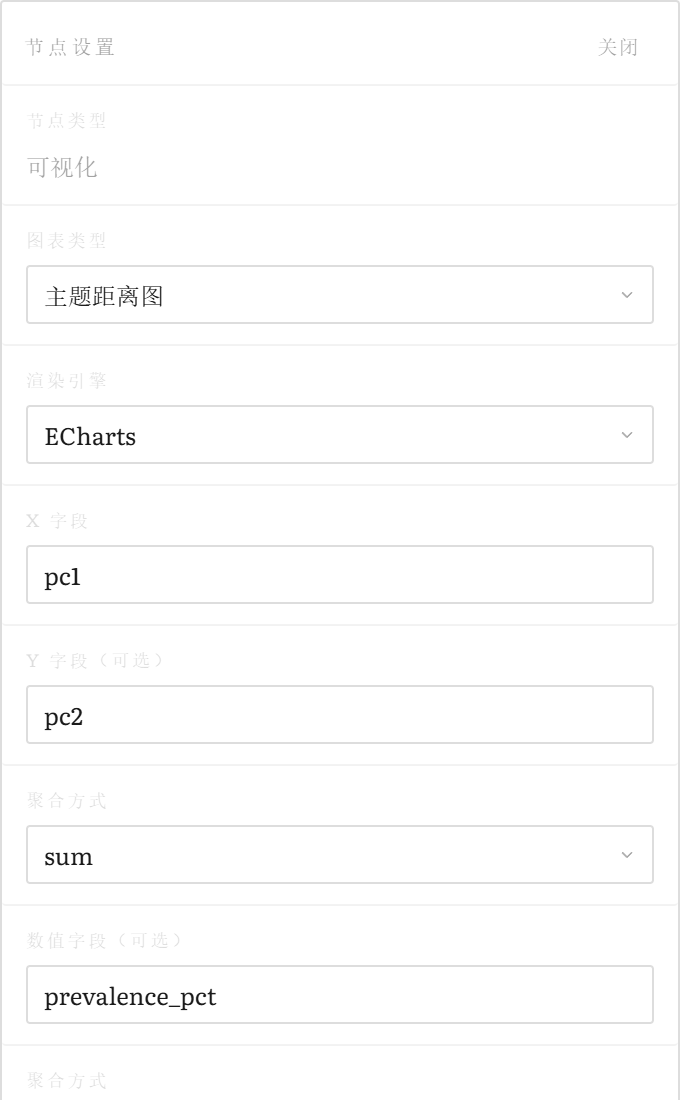
\includegraphics[width=0.31\textwidth]{liu-topicmap.png}
\caption{主题距离图的参数：坐标、标签、气泡大小三列都要指定}
\label{fig:liu-topicmap}
\end{figure}

\section{情感演化与预警}

把情感按阶段或按天算成一个指标，再往后推几期，就得到一条可以讲故事的曲线。

“\texttt{情感演化曲线}”输入一列标签一列分数，输出积极、中性、消极的数量与占比，外加一个情感指数。
指数是积极减消极再除以总数，落在负一到一之间；还可以加一列情感强度，由分数与中点的距离换算，衡量情绪有多激烈。
面板里要指定标签列的三种取值，不同模型给的词不一样，有的是 positive 与 negative，有的是中文，所以这一步不能猜，必须写成实际的值。

分组列选日期得到每日曲线，选阶段得到阶段之间的对比，两个都跑一遍很常见：一张看形状，一张看结论。
有阶段序号时把序号列也填上，否则中文阶段名会被排错。

\begin{figure}[H]\centering
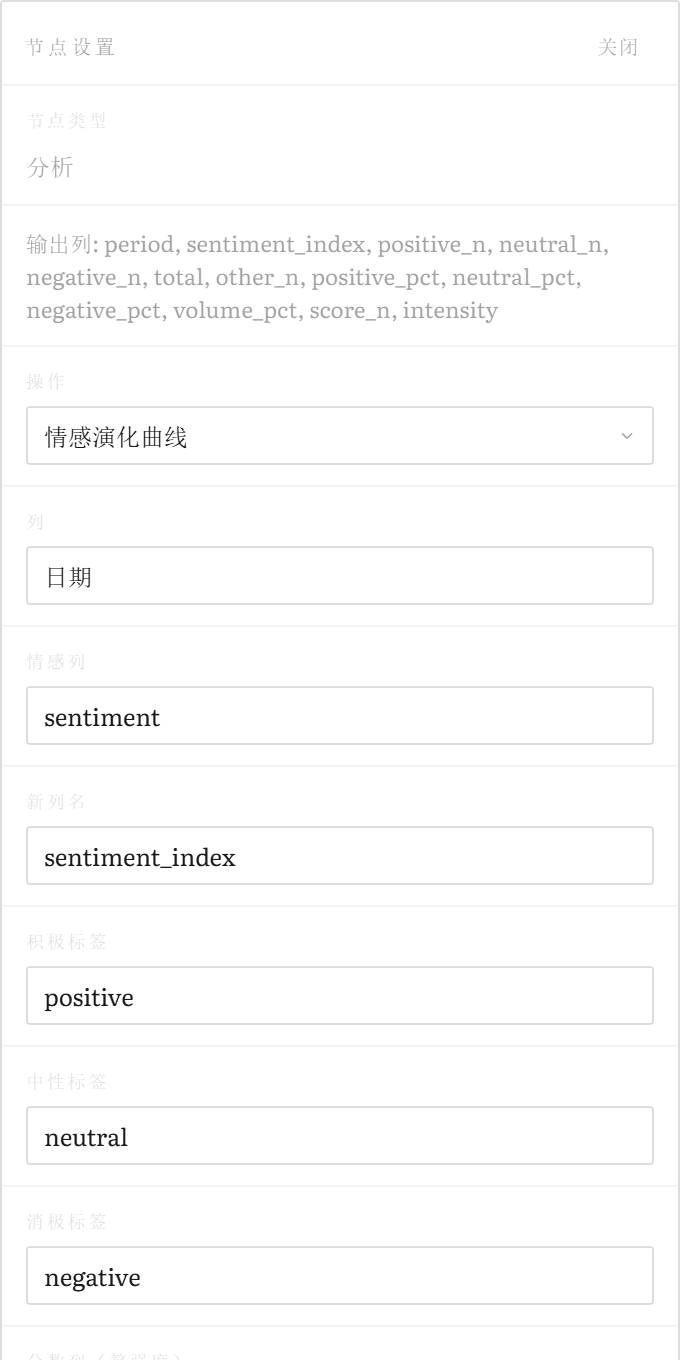
\includegraphics[width=0.31\textwidth]{liu-evolution.png}
\caption{情感演化节点：标签、分数、分组、序号四组参数}
\label{fig:liu-evolution}
\end{figure}

“\texttt{情感走向外推}”把曲线往后推若干期，两种方法，移动平均与 Holt 指数平滑，都是手算，不依赖额外库。
时段列必须能解析成日期，“发酵期”这种名字没法外推，直接拒绝。它推的是曲线的形状，不是预言。

“\texttt{二次爆发预警}”把人的判断写成一条规则。转向是连续若干期同向超过阈值，升温是情感强度每一步都在涨，
两个条件都要求热度还在。一条都没触发时也会给一行未触发，并带上实测到的最大幅度。

\begin{figure}[H]\centering
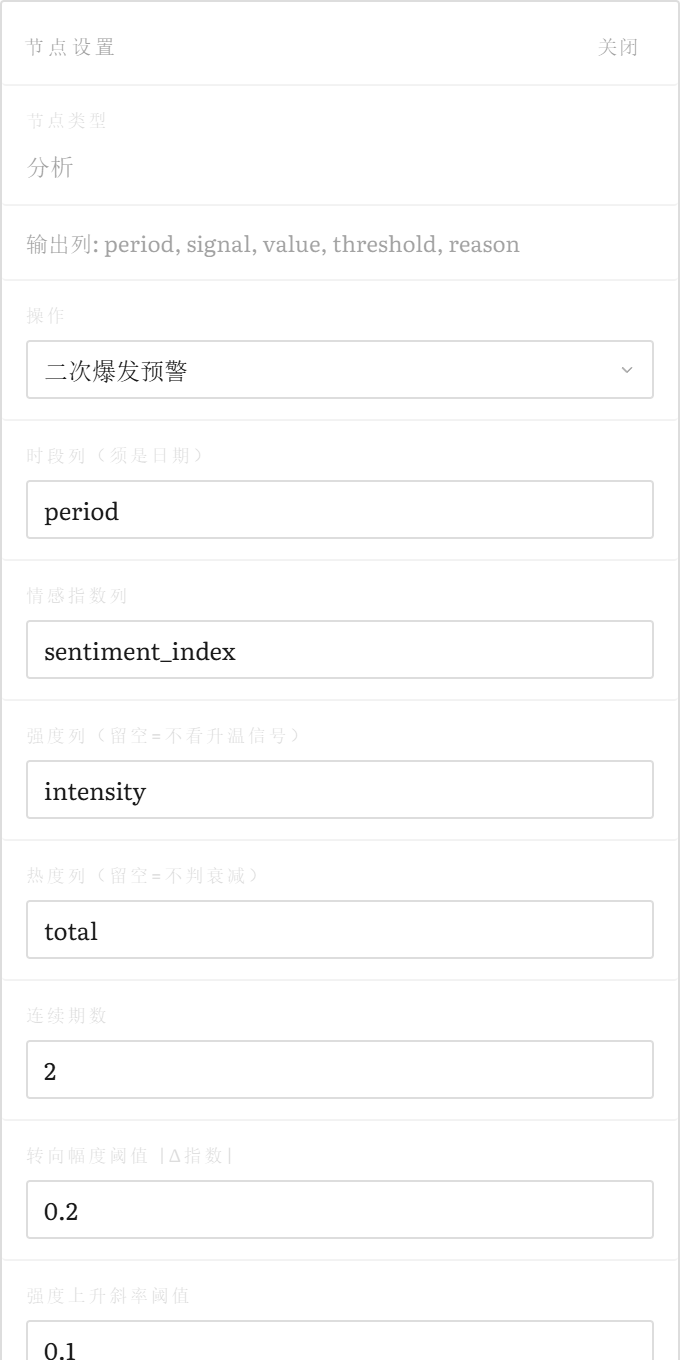
\includegraphics[width=0.31\textwidth]{liu-alert.png}
\caption{二次爆发预警：阈值、连续期数、热度下限}
\label{fig:liu-alert}
\end{figure}

刘学州那次运行里，预警在二月二十二日捕捉到一次转向加升温，强度斜率超过阈值，但当期声量只有三条，
低于前两期均量的六成，所以标成已抑制。四天以后声量配合上来，二次爆发才真正成形。
预警看的是两件事：情绪先行，声量确认。

\section{刘学州事件的完整研究}

仓库里“\texttt{刘学州-评论-情感演化分析-BERT}”有一百七十二个节点，从五份评论 CSV 做到论文里的图和表。
不必照抄全部，看懂它怎么分段就够了：先做一份干净总表，再在总表上派生指标，最后把同一个套路复制到五个阶段。

\subsection{第一段\quad 合并与清洗}

最左边五个上传节点各挂一份评论 CSV，汇到一个输出节点合并成总表。后面接清洗、筛选保留行、归一化去重、近重复去重四步。
每一步都留一个输出节点，中间结果随时能翻出来对账，出问题能定位到具体哪一步把行弄丢了。

\begin{figure}[H]\centering
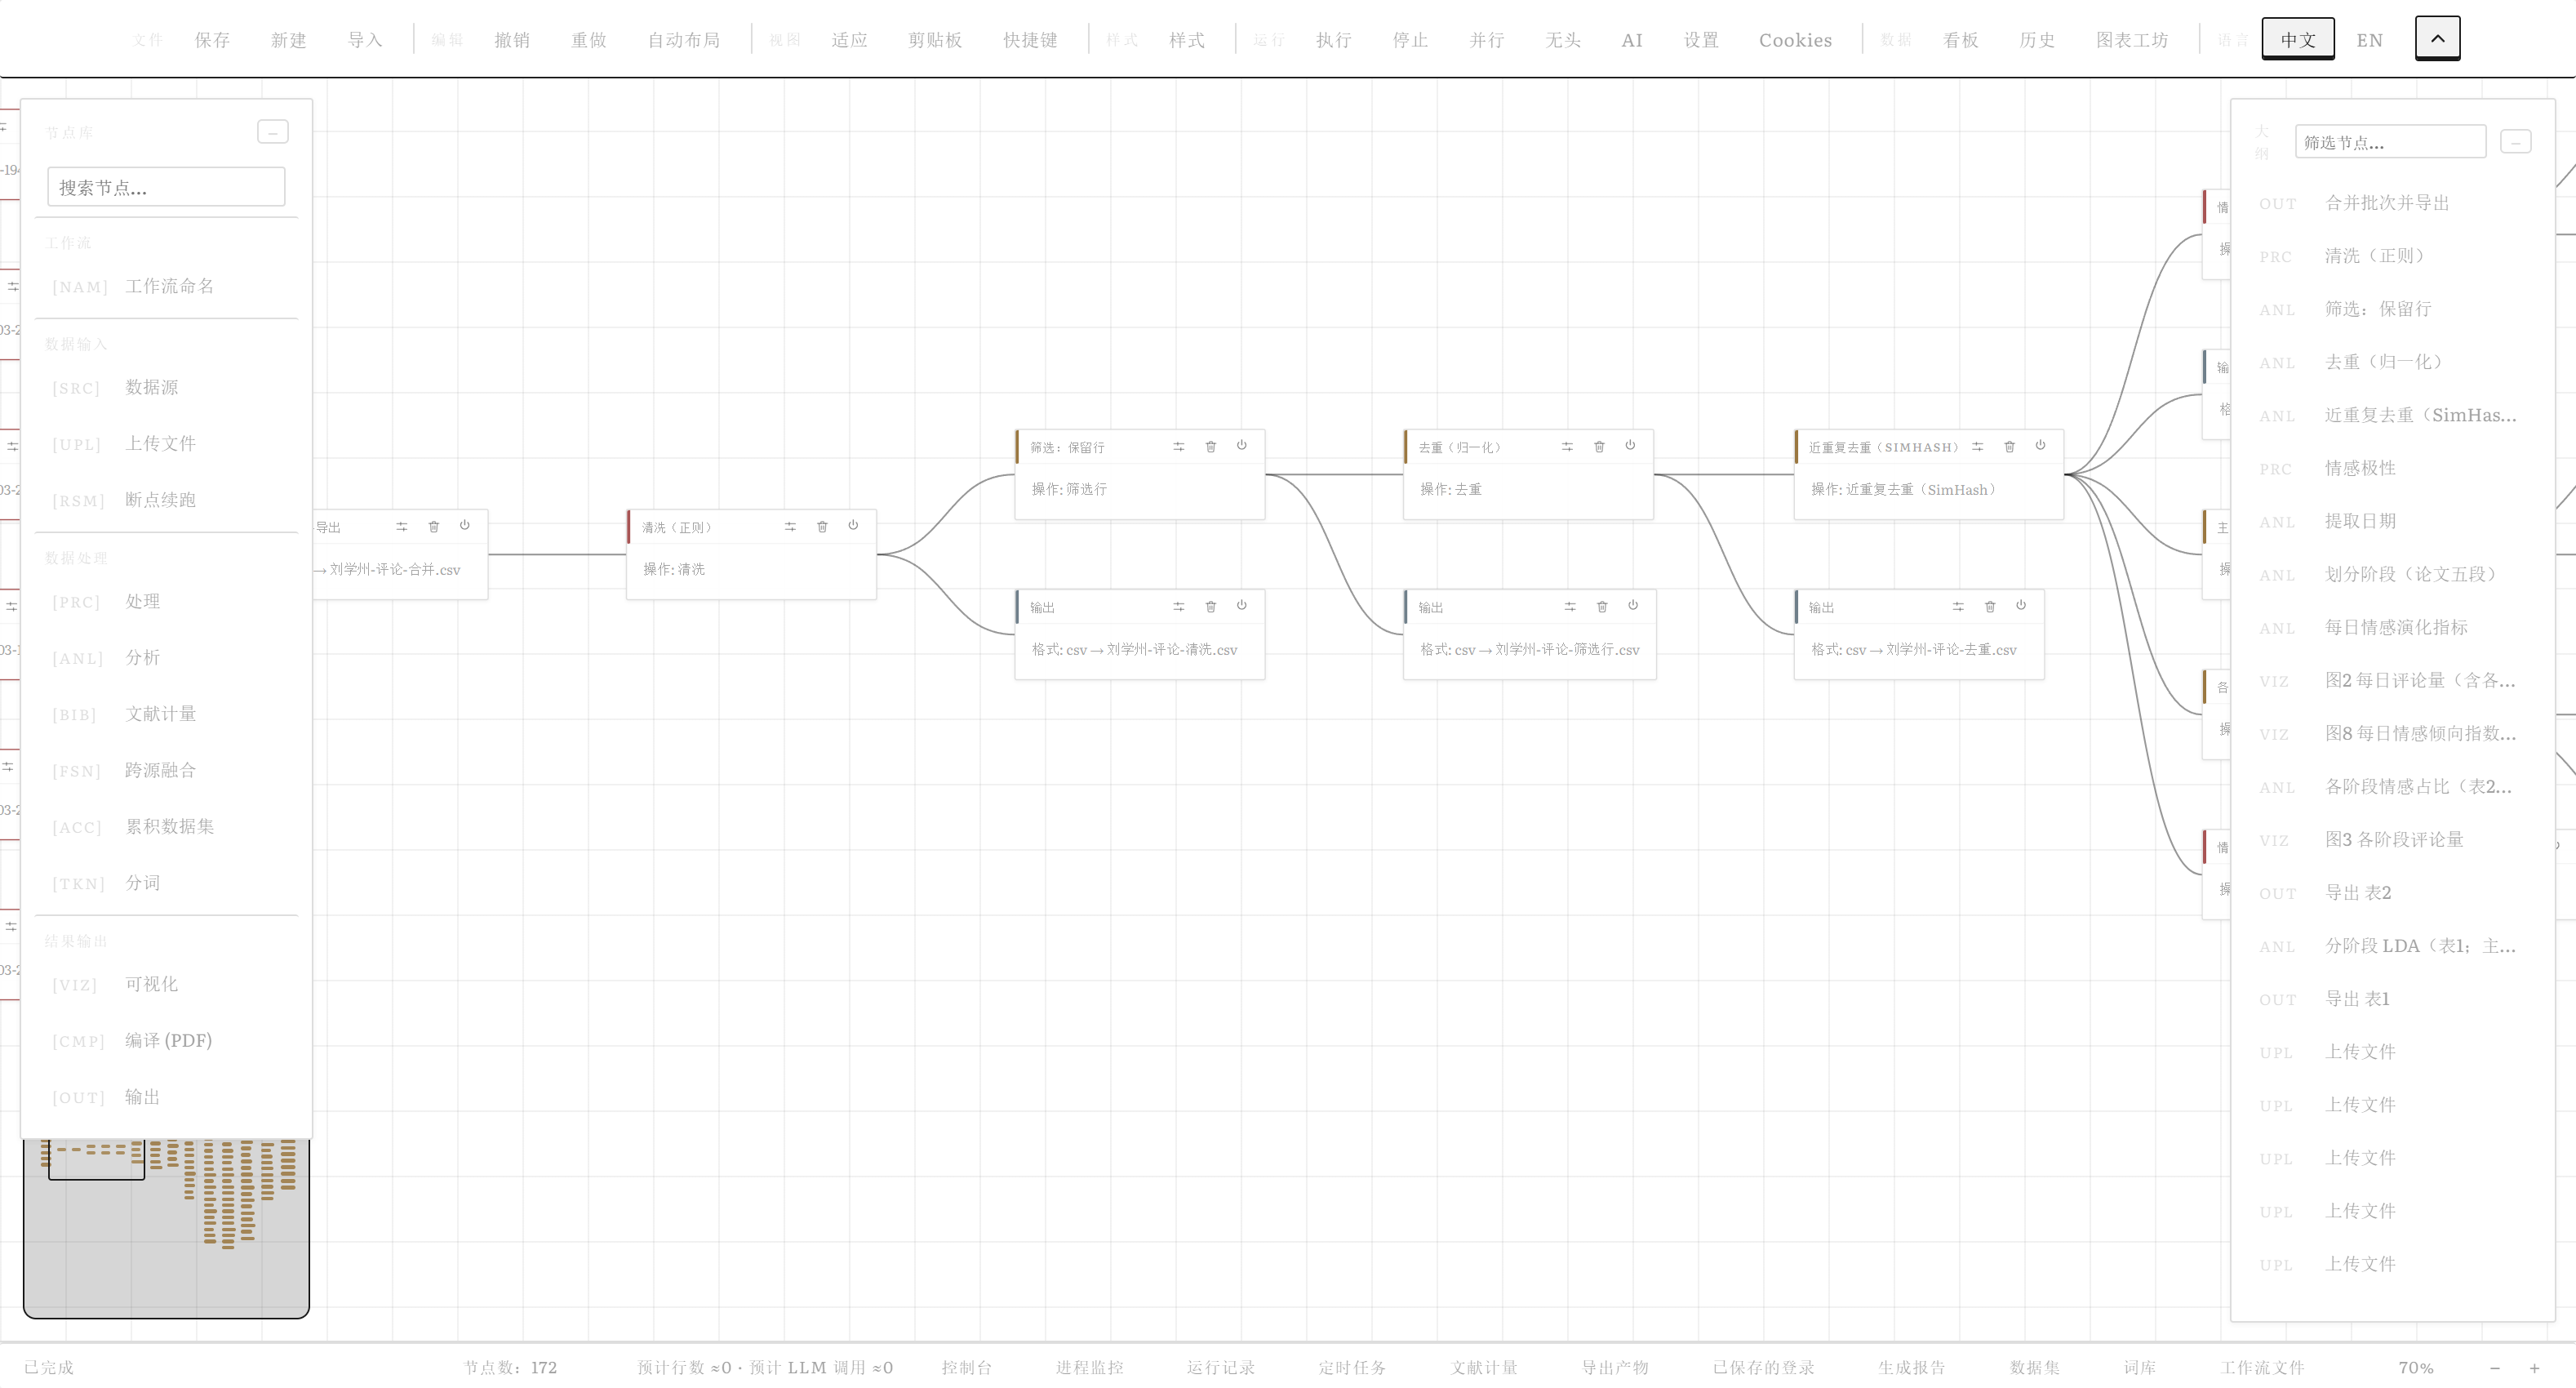
\includegraphics[width=0.98\textwidth]{liu-zoom-clean.png}
\caption{合并、清洗、三层去重，每一步都留一份 CSV 对账}
\label{fig:liu-clean}
\end{figure}

\subsection{第二段\quad 打分与分阶段}

情感极性用微调模型整列推理，正负阈值 0.6 与 0.4，结果写进标签与分数两列。接着提取日期，按六条边界切出五个阶段，
阶段序号一并写出来。阶段边界来自论文，不是程序猜的；想自己定边界时，先用建议边界那个算子看曲线。

\begin{figure}[H]\centering
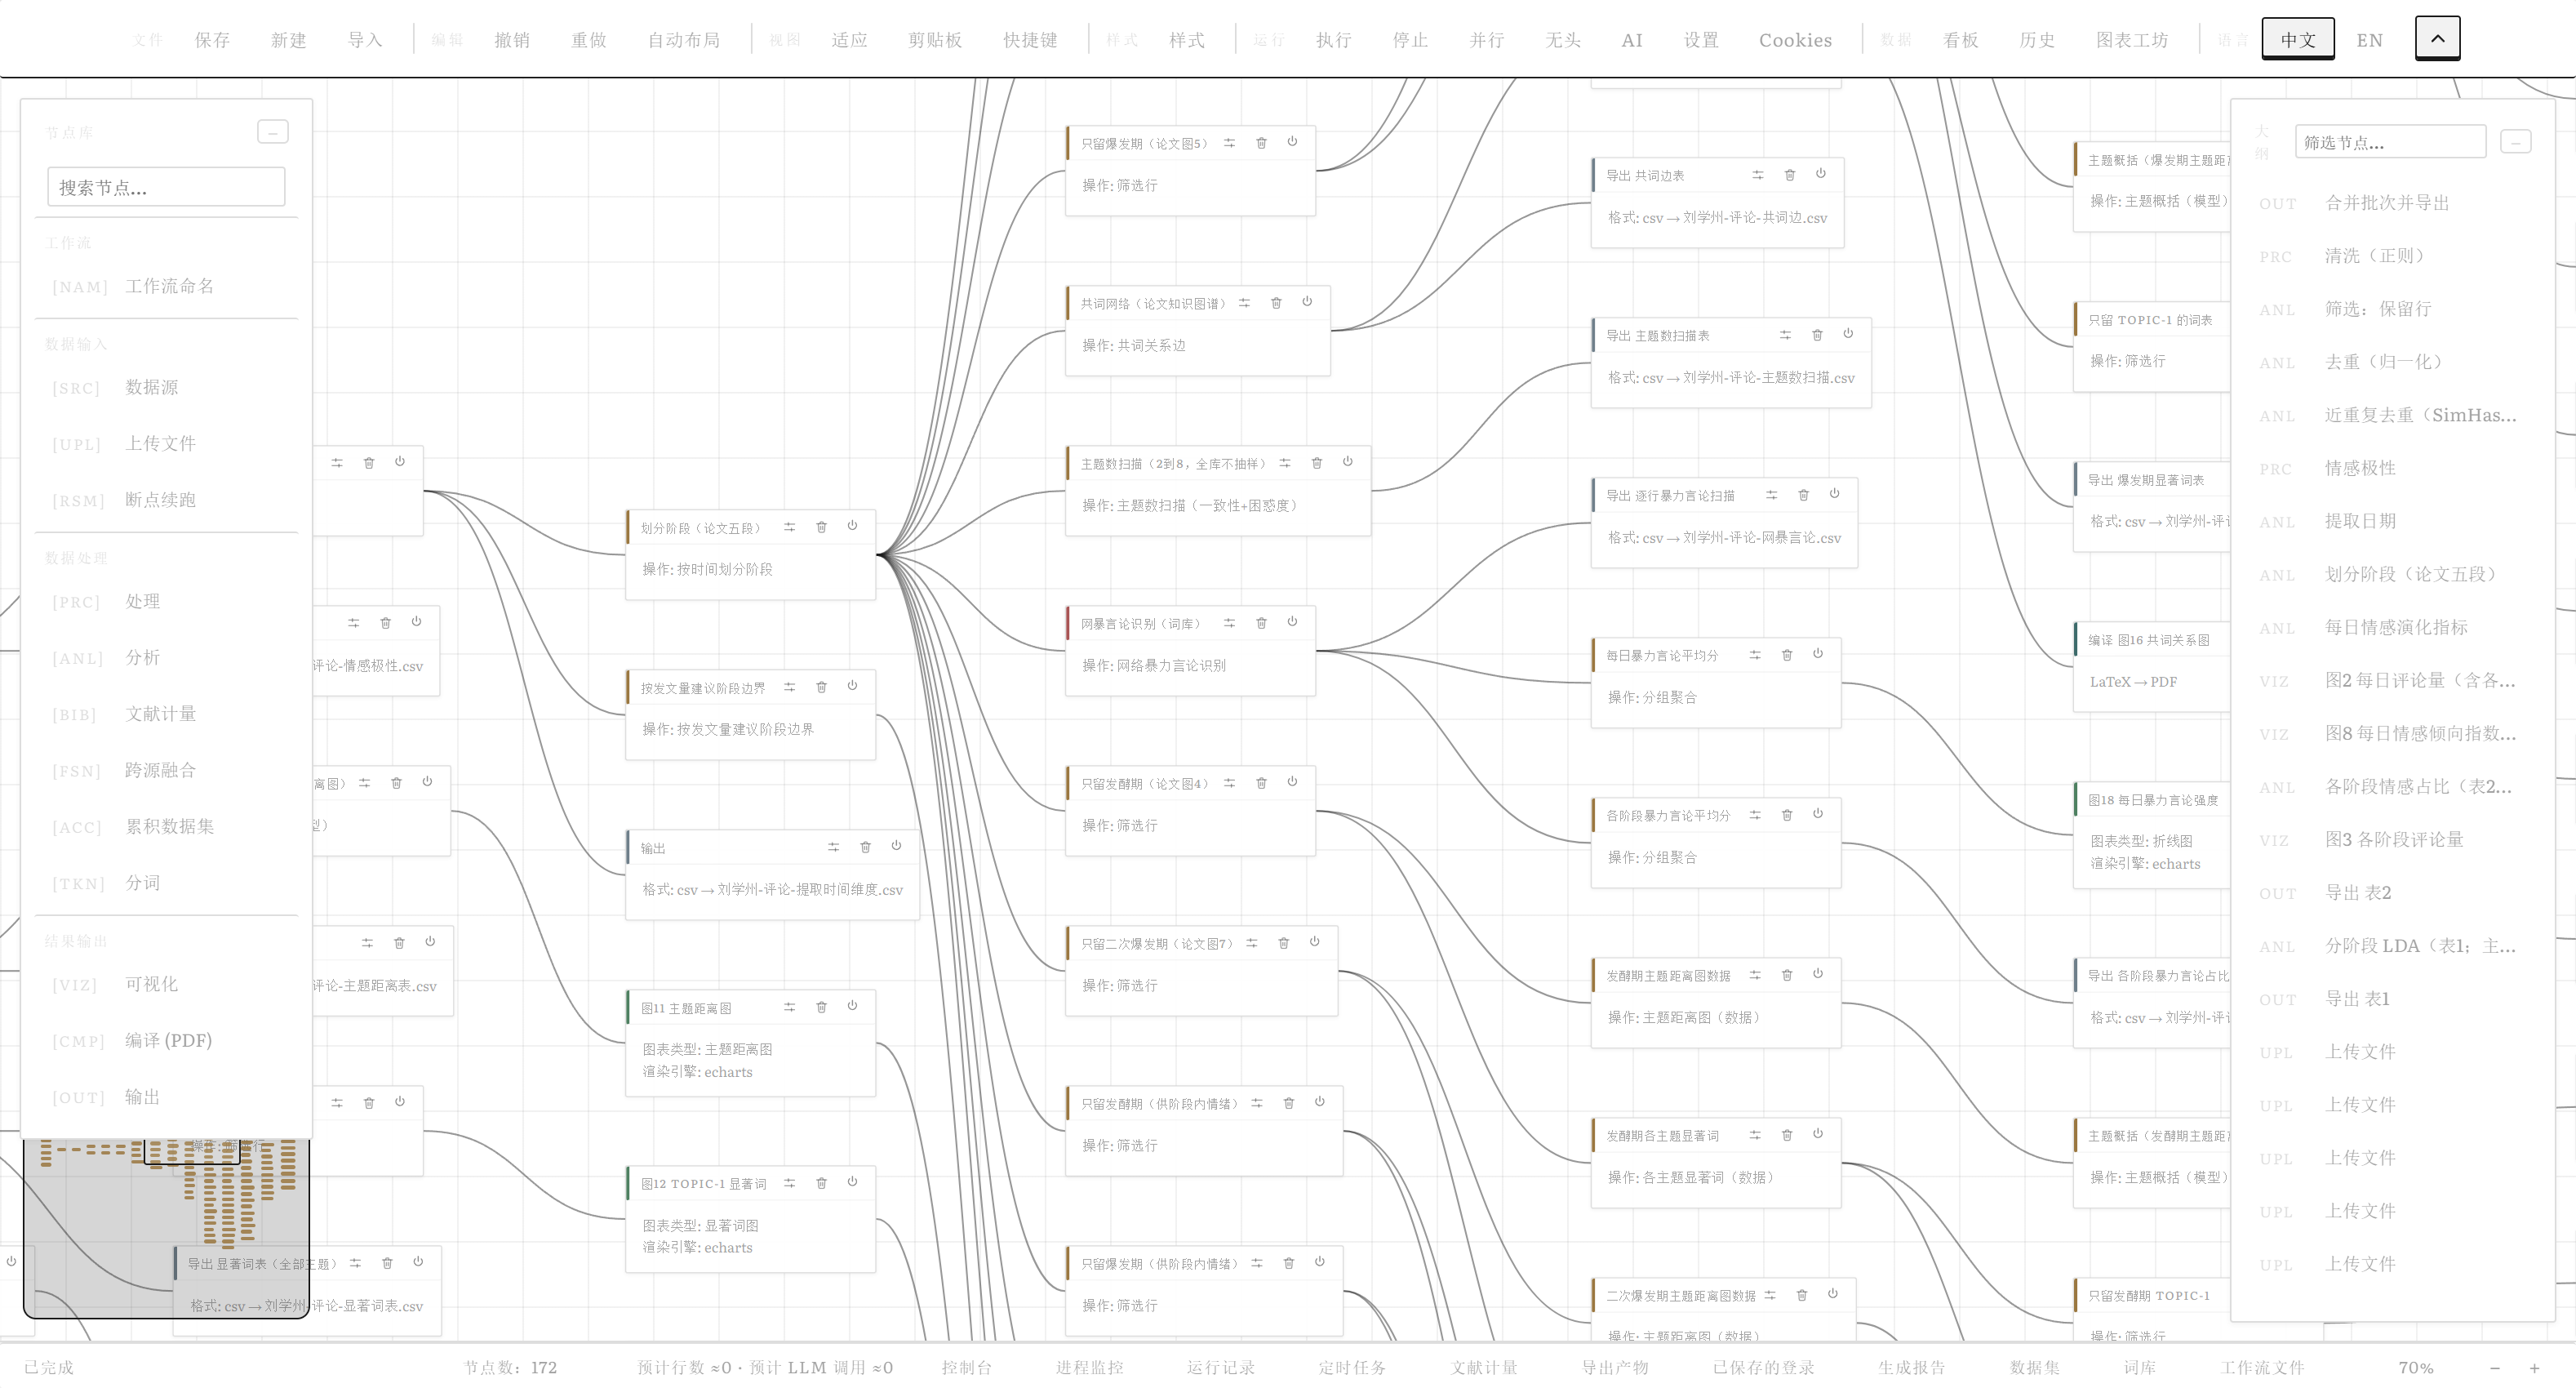
\includegraphics[width=0.98\textwidth]{liu-zoom-stage.png}
\caption{划分阶段把一张总表分成五个分支，每个分支一套主题与情感图}
\label{fig:liu-stage-branch}
\end{figure}

\subsection{第三段\quad 主线的四张图}

每日评论量、每日情感指数、各阶段评论量、各阶段情感占比，四张图构成主线的证据。每日评论量那张带事件标注，
几个峰值日上画竖虚线并写一句话，标注的位置必须与横轴取值一字不差，对不上会拒绝并列出可选值。

\subsection{第四段\quad 主题}

分阶段主题、主题概括、主题距离、显著词、生命周期、流向、共词网络一路做下来。主题距离图用气泡大小表示占比，
标签用概括那一列，不是 Topic-1 这种编号。

\subsection{第五段\quad 预警与攻击性}

情感走向外推与二次爆发预警各一条链。网暴言论识别单独一条，按日期与阶段各聚合一次，得到每日攻击性均值与各阶段对比。

\subsection{第六段\quad 分阶段复制}

同一个套路在五个阶段各复制一遍，每段有自己的主题图、显著词、阶段内情感曲线。节点多，但结构重复，学会一段就会五段。
中间任何一步都能单独重跑，下游自动复用没变的部分。

\subsection{这条工作流教了什么}

三段式。先做一份干净的总表，再在总表上派生各种指标，最后复制成图。长链的关键步骤都留一个输出节点，
每个阶段的结论都能落成文件，论文里的每个数字都能顺着文件找回它是哪一次运行、哪一列算出来的。

\section{文献计量}

文献计量节点吃的是题录表，不是全文。上游可以是上传的导出文件，也可以是爬回来的表；列名不一样也没关系，
节点里有一张列映射，把任意表的列接到它认识的字段上。

\begin{table}[H]\centering
\caption{能识别的文献导出件}
\label{tab:biblio-formats}
\small
\begin{tabularx}{\textwidth}{p{3.0cm}X}
\toprule
来源 & 说明 \\
\midrule
中国知网 & 三种导出按钮都认：RefWorks 文本、NoteExpress、EndNote \\
CSSCI & 文本导出，中文表头 \\
Web of Science & 纯文本全记录、Excel、RIS、BibTeX \\
Scopus & CSV，中英文表头都认 \\
Dimensions & CSV，要选全记录导出 \\
Lens & 学术文献集合的 CSV \\
PubMed & Medline 文本与 CSV 摘要，没有 XML 读法 \\
其他 & RIS、BibTeX、EndNote、NoteExpress \\
\bottomrule
\end{tabularx}
\end{table}

统一之后的列有记录编号、题名、作者、单位、来源期刊、年份、卷期页码、关键词、摘要、参考文献、DOI 与格式，
再按实际数据追加国家、学科、引用次数、使用次数、基金、文献类型、语言。

几条边界是硬性的。知网的 RefWorks 通常没有参考文献，所以引文网络与共被引建不起来；Lens 的专利集合会被拒绝，
它的引用列写的是记录编号而不是引文文本；Web of Science 的 Excel 缺参考文献整列，能建关键词与学科网络，建不了引文网络。

\section{建网与指标}

节点里先选实体。关键词、作者、机构、国家、学科、主题词、基金做共现，文献、作者、期刊做共被引，还有文献耦合与期刊耦合。
共现类只要实体列与年份列，引文类要参考文献列。

\subsection{时间切片}

按年份切片，每片按 TopN、Top 百分比、g-index 或阈值三元组挑选，再合并。可以设回溯年数、最低被引数、引文扩展的阶数。
切片让早年的小网络与近年的大网络都不至于被对方淹没。

\subsection{剪枝}

边太多时图会糊成一团。三种剪法：不剪、最小生成树、Pathfinder。Pathfinder 有三个参数：距离的范数、间接路径最多几跳、保留比例。
默认在每片内部剪完再合并，也可以合并以后一次剪。

\subsection{指标}

每个节点算度、中介中心性、特征向量中心性、PageRank 与 Sigma。输入带被引次数时追加总被引与 h 指数，带使用次数时追加使用次数合计。
中介中心性在节点很多时按抽样估算，控制台会写明抽了多少个源点。

\begin{figure}[H]\centering
\begin{tikzpicture}[scale=0.9]
  \foreach \a/\b in {0/1,0/2,1/2,1/3,2/3,3/4,2/4,4/5,3/5,0/5} {
    \pgfmathsetmacro{\xa}{cos(\a*72+18)*1.9}
    \pgfmathsetmacro{\ya}{sin(\a*72+18)*1.9}
    \pgfmathsetmacro{\xb}{cos(\b*72+18)*1.9}
    \pgfmathsetmacro{\yb}{sin(\b*72+18)*1.9}
    \draw[draw=cA!45,line width=0.8pt] (\xa,\ya) -- (\xb,\yb);
  }
  \foreach \a/\r in {0/0.26,1/0.34,2/0.22,3/0.30,4/0.20,5/0.24} {
    \pgfmathsetmacro{\xa}{cos(\a*72+18)*1.9}
    \pgfmathsetmacro{\ya}{sin(\a*72+18)*1.9}
    \fill[cA!60] (\xa,\ya) circle (\r);
    \draw[draw=cA] (\xa,\ya) circle (\r);
  }
  \node[tag] at (0,-2.4) {圆的大小是频次，线的粗细是共现强度，位置由布局算定};
\end{tikzpicture}
\caption{知识图谱的样子}
\label{fig:kg}
\end{figure}

\subsection{聚类、突现与变异}

聚类用谱聚类，簇数留空时按特征值间隙自动选。簇名可以用 LLR、LSI、互信息或 TF-IDF 生成，也可以用手工标签覆盖。
突现按逐年文档数算，每个节点保留最强的一段区间，另写一张突现词表。结构变异比较相邻两期连边分布的散度，
只有两期都存在的节点才计分，切片不连续时不跨缺口比较。

情感叠加与话题叠加需要上游已经写好的标签列。每个节点追加两列，一列是主导标签，一列是各标签的篇数分布；
分母只算有标签的文档，空白是没有判断，不当中性。

\subsection{输出与图}

默认输出一行一节点的实体表，也能单独输出边表、簇表、突现表与双图叠加表。成图有十四种：知识图谱、环形图、聚类时间线、景观图、
突现词图、时区图、聚类年份热力图、三维图谱、结构变异图、双图叠加、情感叠加、话题叠加、国家地理图、同心环。

每张图都另出一份 TikZ 源与一份三线表。图谱与环形图还带按年份回放：拖动底下那条滑杆，节点按到那一年为止的累计频次长大，
最后一帧与完整图完全一致。

\section{AIGC 的文献计量}

这一段从知网采集开始，到四张图结束。打开“\texttt{AIGC文献计量（知网自动采集3000篇·去重清洗）}”。

\begin{figure}[H]\centering
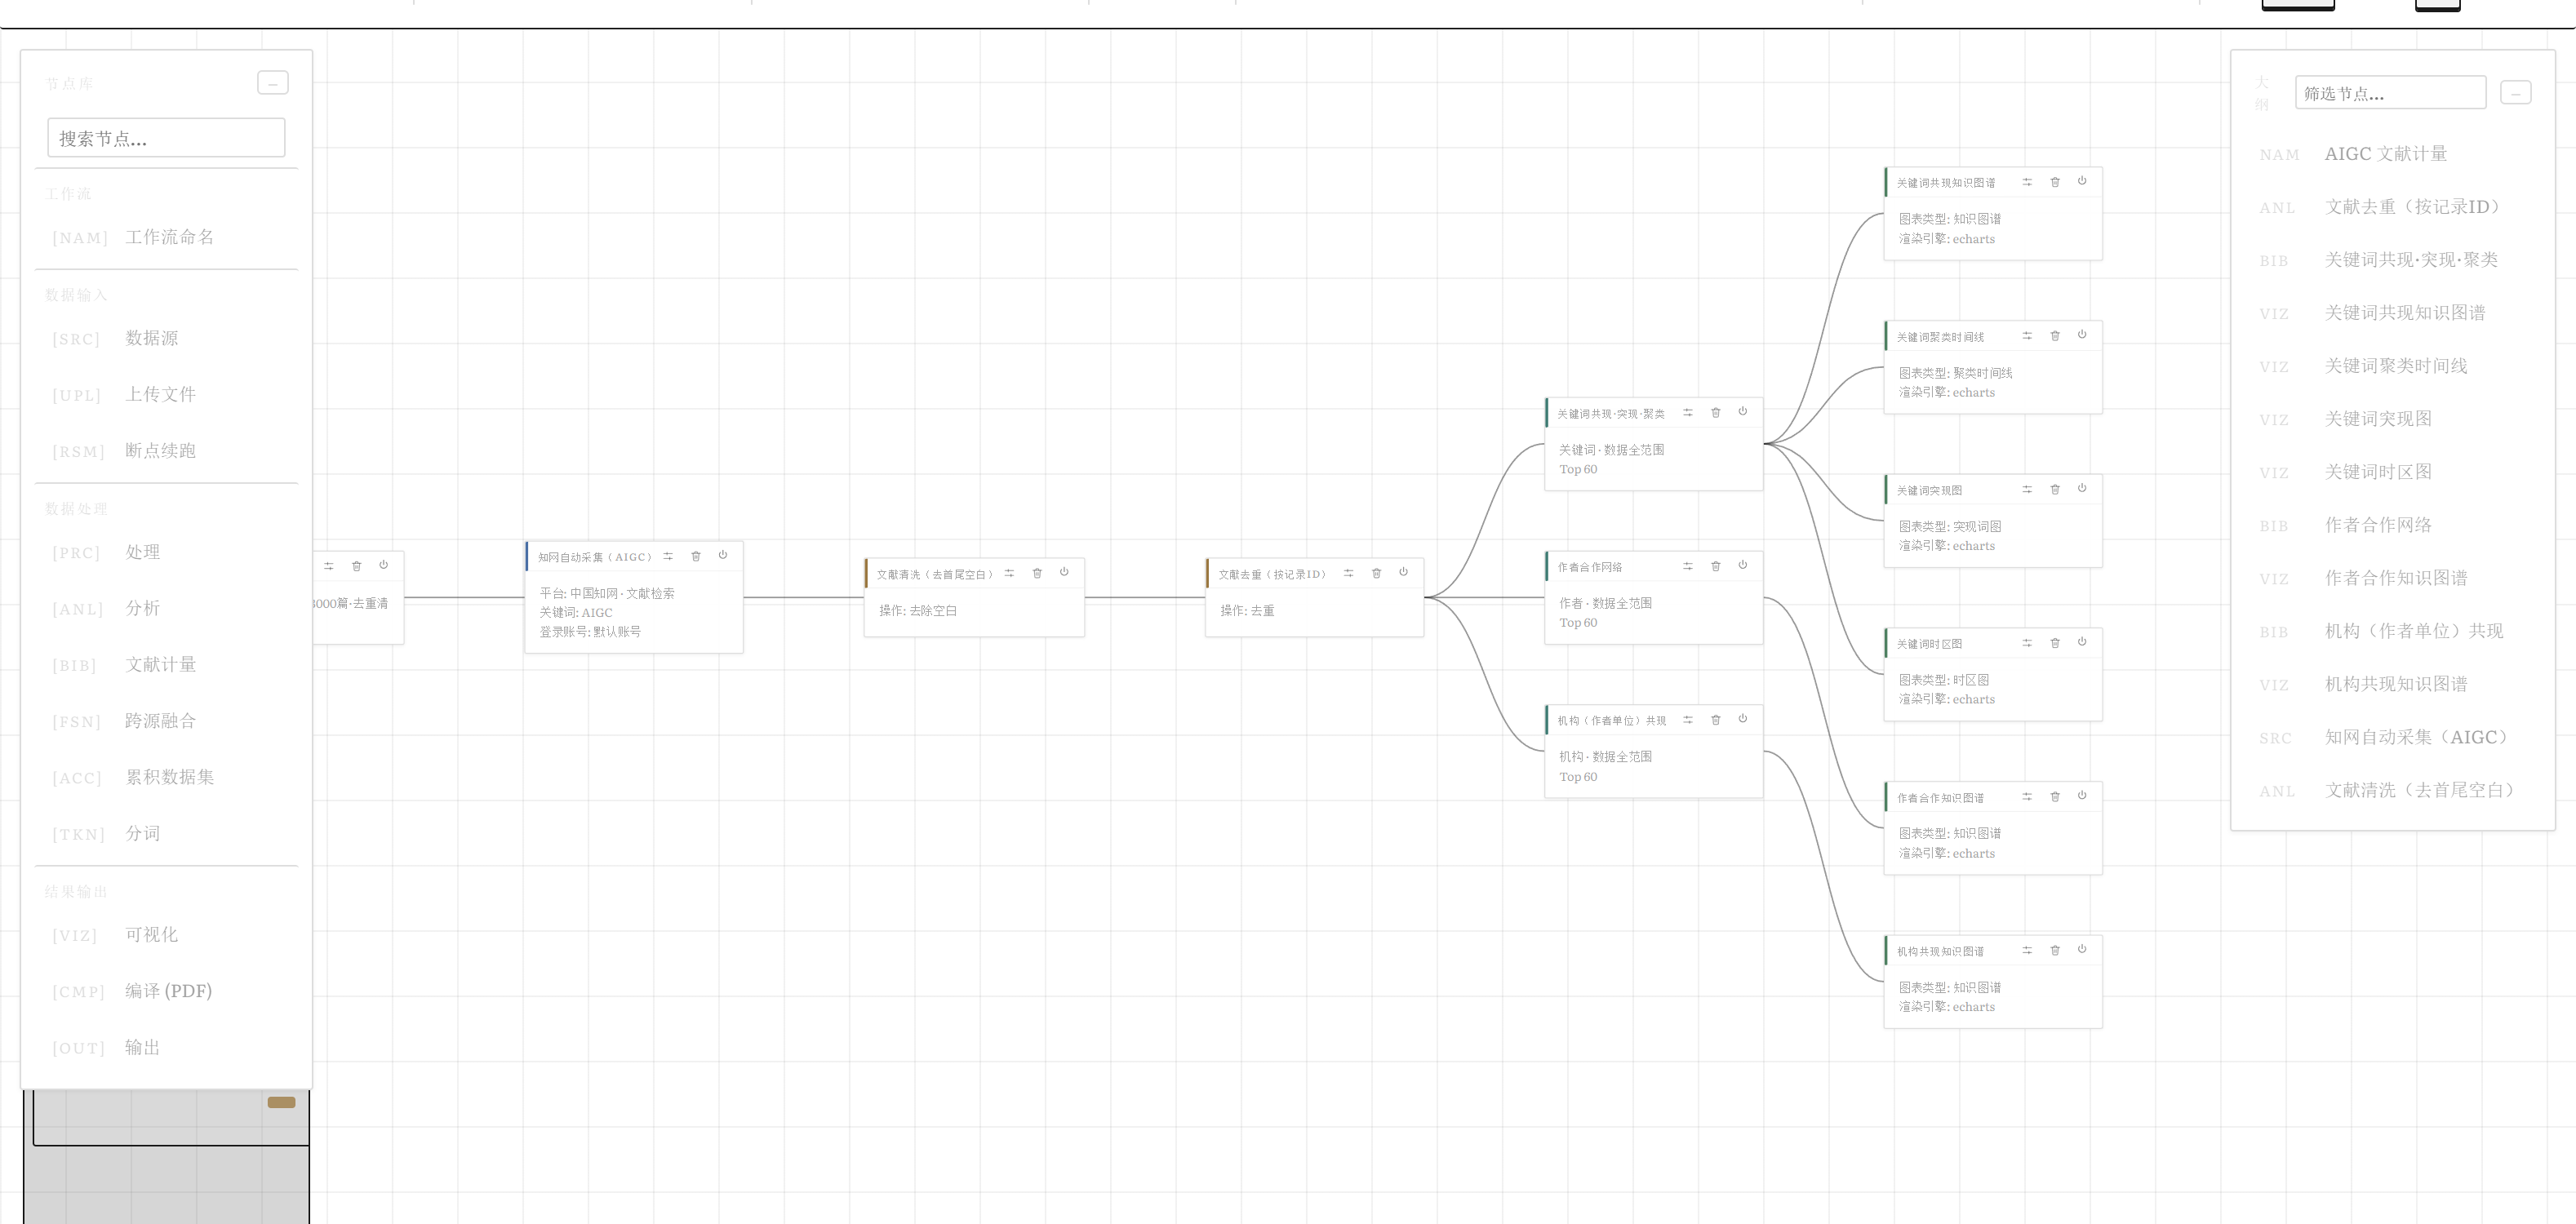
\includegraphics[width=0.98\textwidth]{bib-canvas.png}
\caption{AIGC 文献计量：采集、去重、三路建网、四张图}
\label{fig:bib-canvas}
\end{figure}

\subsection{采集}

数据源选“\texttt{中国知网}”，关键词 \texttt{AIGC}，目标三千篇。知网的全选只作用于当页，程序逐页点一次全选再导出，
所以篇数能走到你填的数。

\subsection{清洗}

采回来的题录先过一遍去重，按记录编号判重；再过一遍去空白，把题名、作者、单位、期刊、关键词、摘要、DOI 这几列的空白去掉。
列名在这里要逐字对上，写错会被拒绝并列出实际有哪些列。

\subsection{建网}

中间那个文献计量节点建关键词网：实体选关键词，最少出现两次，按 TopN 选点，余弦相似度，最小生成树剪枝，按五年切片，开聚类与突现。
输出实体表，同时把图谱、边表、簇表、突现表都写成文件。

\begin{figure}[H]\centering
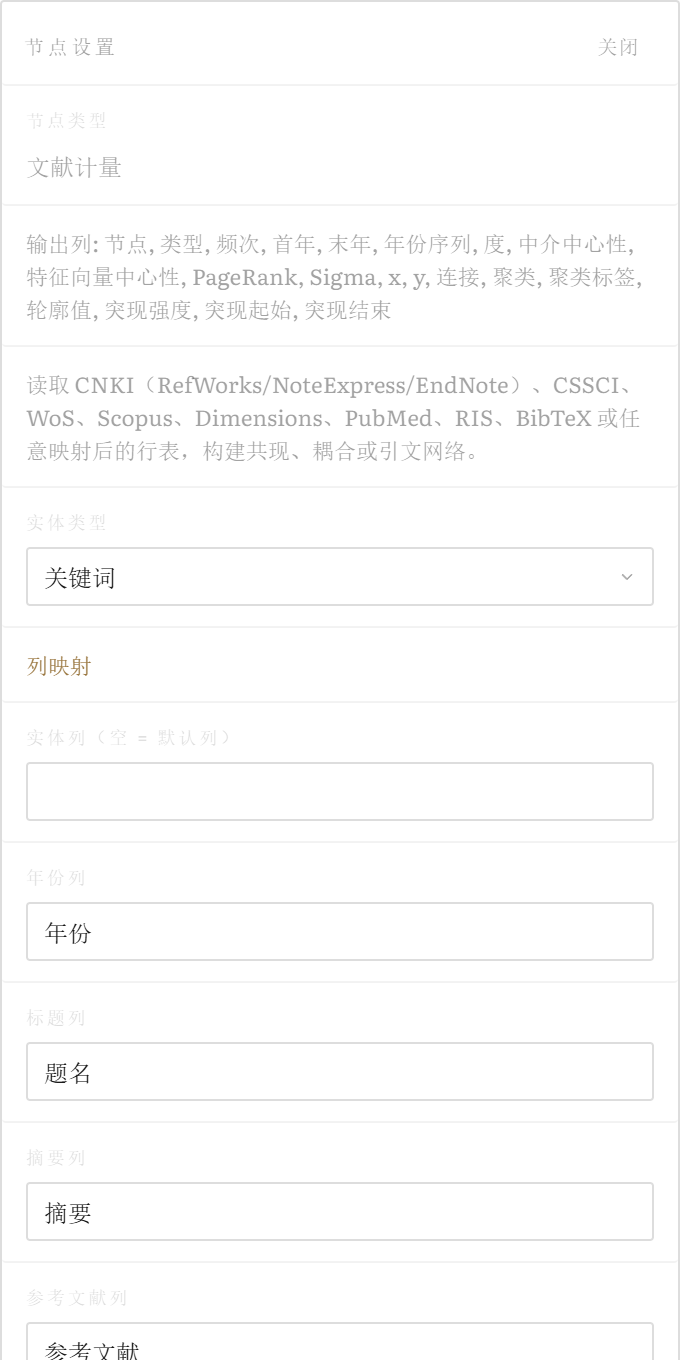
\includegraphics[width=0.31\textwidth]{bib-node.png}
\caption{文献计量节点：实体、切片、选择、剪枝、聚类都在这一屏}
\label{fig:bib-node}
\end{figure}

右边两个节点分别建作者网与机构网，参数更简单：最少一次，不剪枝，取前六十。三条网共用同一份题录，
所以只要采集与清洗跑过一次，后面可以反复调参数重跑，不用再上站点。

\subsection{出图}

四个可视化节点分别接三条网，图表类型选知识图谱、聚类时间线、突现词图、时区图。每个节点里“\texttt{生成 LaTeX 图}”默认开着，
所以除了屏幕上的图，还会在导出目录留下可以编译的图源。后面可以再接一个编译节点，把图与表合成一份 PDF。

\begin{figure}[H]\centering
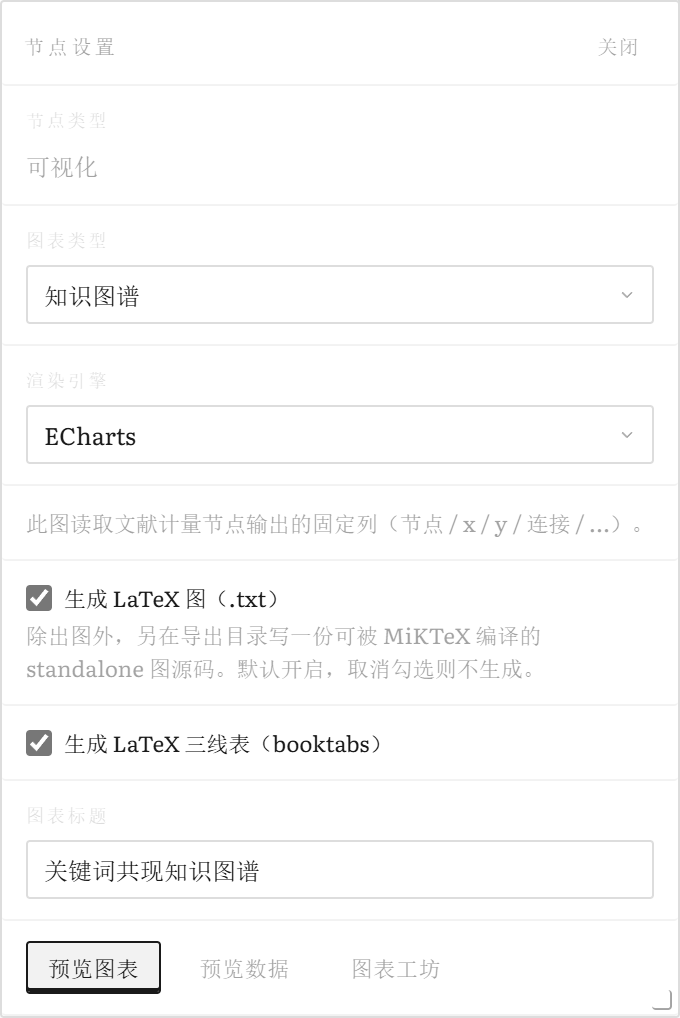
\includegraphics[width=0.31\textwidth]{bib-graph.png}
\caption{可视化节点里的图表类型与 LaTeX 选项}
\label{fig:bib-graph}
\end{figure}

\subsection{跨运行监测}

在文献计量节点里填一个监测项目名，每次运行都会把这张网存成该项目的一份快照，并与上一次对比：
新增与消失的节点、新增与消失的连边、变了的属性、新簇与结束的突现、动过的参数，逐条打印并另存一份表。
配上定时任务，就是一条领域监测线。

\section{跨源融合与长期积累}

“\texttt{跨源融合}”节点吃多张上游表，把不同来源的记录折成一份规范表。每个字段给一串候选列，按顺序尝试。
文献的关键词与帖子的话题折进同一个词表，下游的文献计量用默认列映射就能读。来源是数据，不是猜的：
表里自带平台或来源列就逐行取，没有就用你为某个父节点写的标签，再没有才按节点编号登记。它不会替一个没说过自己来历的表写文献。

输入表带来源列时，下游文献计量的输出会多两列：一列写这个实体出现在哪些语料，一列写是不是跨语料。
这两列能回答问题：哪些词只在一个语料里，哪些两边都在谈。

一般的输出是每次覆盖一份文件。需要长期攒数据时用“\texttt{累积数据集}”节点，它把每次的新行追加进一份带版本的长期表，
去重方式要显式选，列变了按名字拒绝。适合每天跑一次、一年以后回看的场景。

哔哩哔哩作者投稿这类会持续增长的来源，可以停在上一次运行的边界继续采。程序记住上次采到哪一条，
这次从那里往后走，不重复抓老内容，也不漏掉新内容。

\section{图表}

可视化节点的图表类型有三十种，另加十四类文献图谱。

\begin{table}[H]\centering
\caption{图表分组}
\label{tab:charts}
\small
\begin{tabularx}{\textwidth}{p{2.4cm}X}
\toprule
分组 & 图表 \\
\midrule
比较 & 柱状、条形、箱线、雷达 \\
趋势 & 折线、双轴折线、面积、占比堆叠 \\
分布 & 直方、散点、气泡、热力图、小提琴 \\
关系 & 桑基、关系网络、和弦、主题流向 \\
文本 & 词云、显著词、共词网络 \\
地理与时间 & 中国地图、国家地理图、时间线、时区 \\
研究 & 主题距离、模型一致率、突现词、结构变异、双图叠加、同心环 \\
\bottomrule
\end{tabularx}
\end{table}

\subsection{两个引擎}

ECharts 在浏览器里画，交互好、速度快；Matplotlib 在服务端画，适合批量出图。一部分图只有 ECharts 支持，
选错会明说，不会画成别的东西。

\subsection{论文样式}

这套图是按印刷做的，不是仪表盘。颜色低调，衬线字，折线不平滑也不填色阶，只留左边与下面两条坐标轴，网格浅而虚。
分类轴保留表格自己的行序，取值多了会斜排并强制显示每一格。图里的文字、图例、坐标轴名跟着界面语言变；
数据里的列名与标签值不动，那是节点之间的约定。

柱状、折线、双轴折线还能加事件标注，写成一串“日期=名称”，横轴上对应位置画一条竖虚线。
标签必须与轴上的取值一字不差，对不上会拒绝并列出可选的值。

\section{预览、全屏与看板}

可视化节点跑过一次以后，设置底部的“\texttt{预览图表}”就能看。浮层里是真正的图，顶上一排是全屏、存为图片、存为 SVG、关闭；
底部是复制或下载 LaTeX 图源、把图编译成 PDF、复制或下载三线表。

\begin{figure}[H]\centering
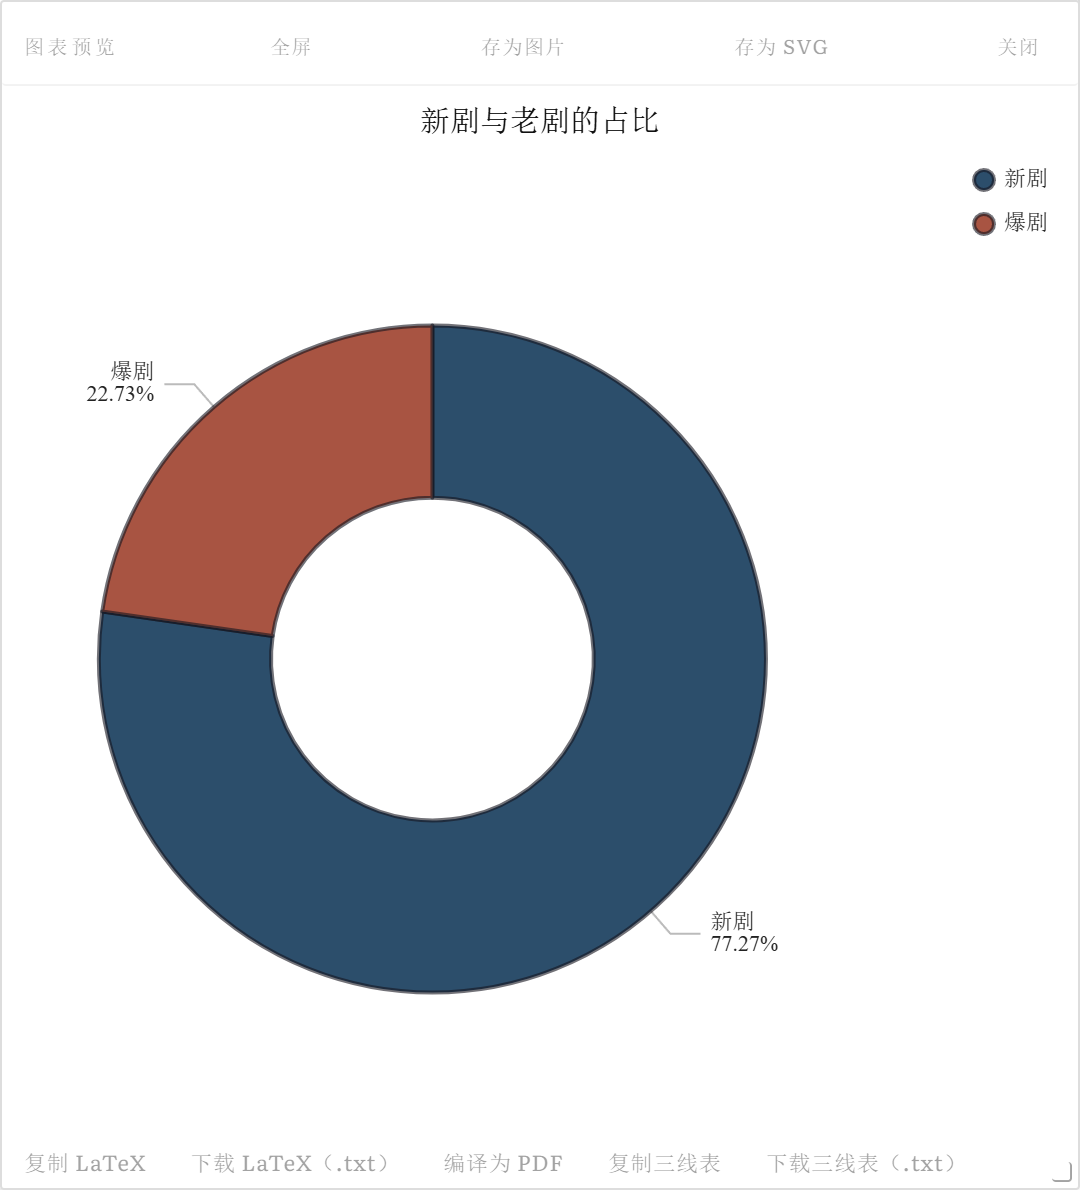
\includegraphics[width=0.84\textwidth]{chart-preview.png}
\caption{图表预览：顶部四个按钮，底部一排 LaTeX 与编译操作}
\label{fig:chart-preview}
\end{figure}

“\texttt{全屏}”把这张图放进一个可拖动、可缩放的浮窗，适合把一页论文大小的图放到最大看细节，也方便直接截图。
窗口顶上同样有存为图片、存为 SVG、关闭。

\begin{figure}[H]\centering
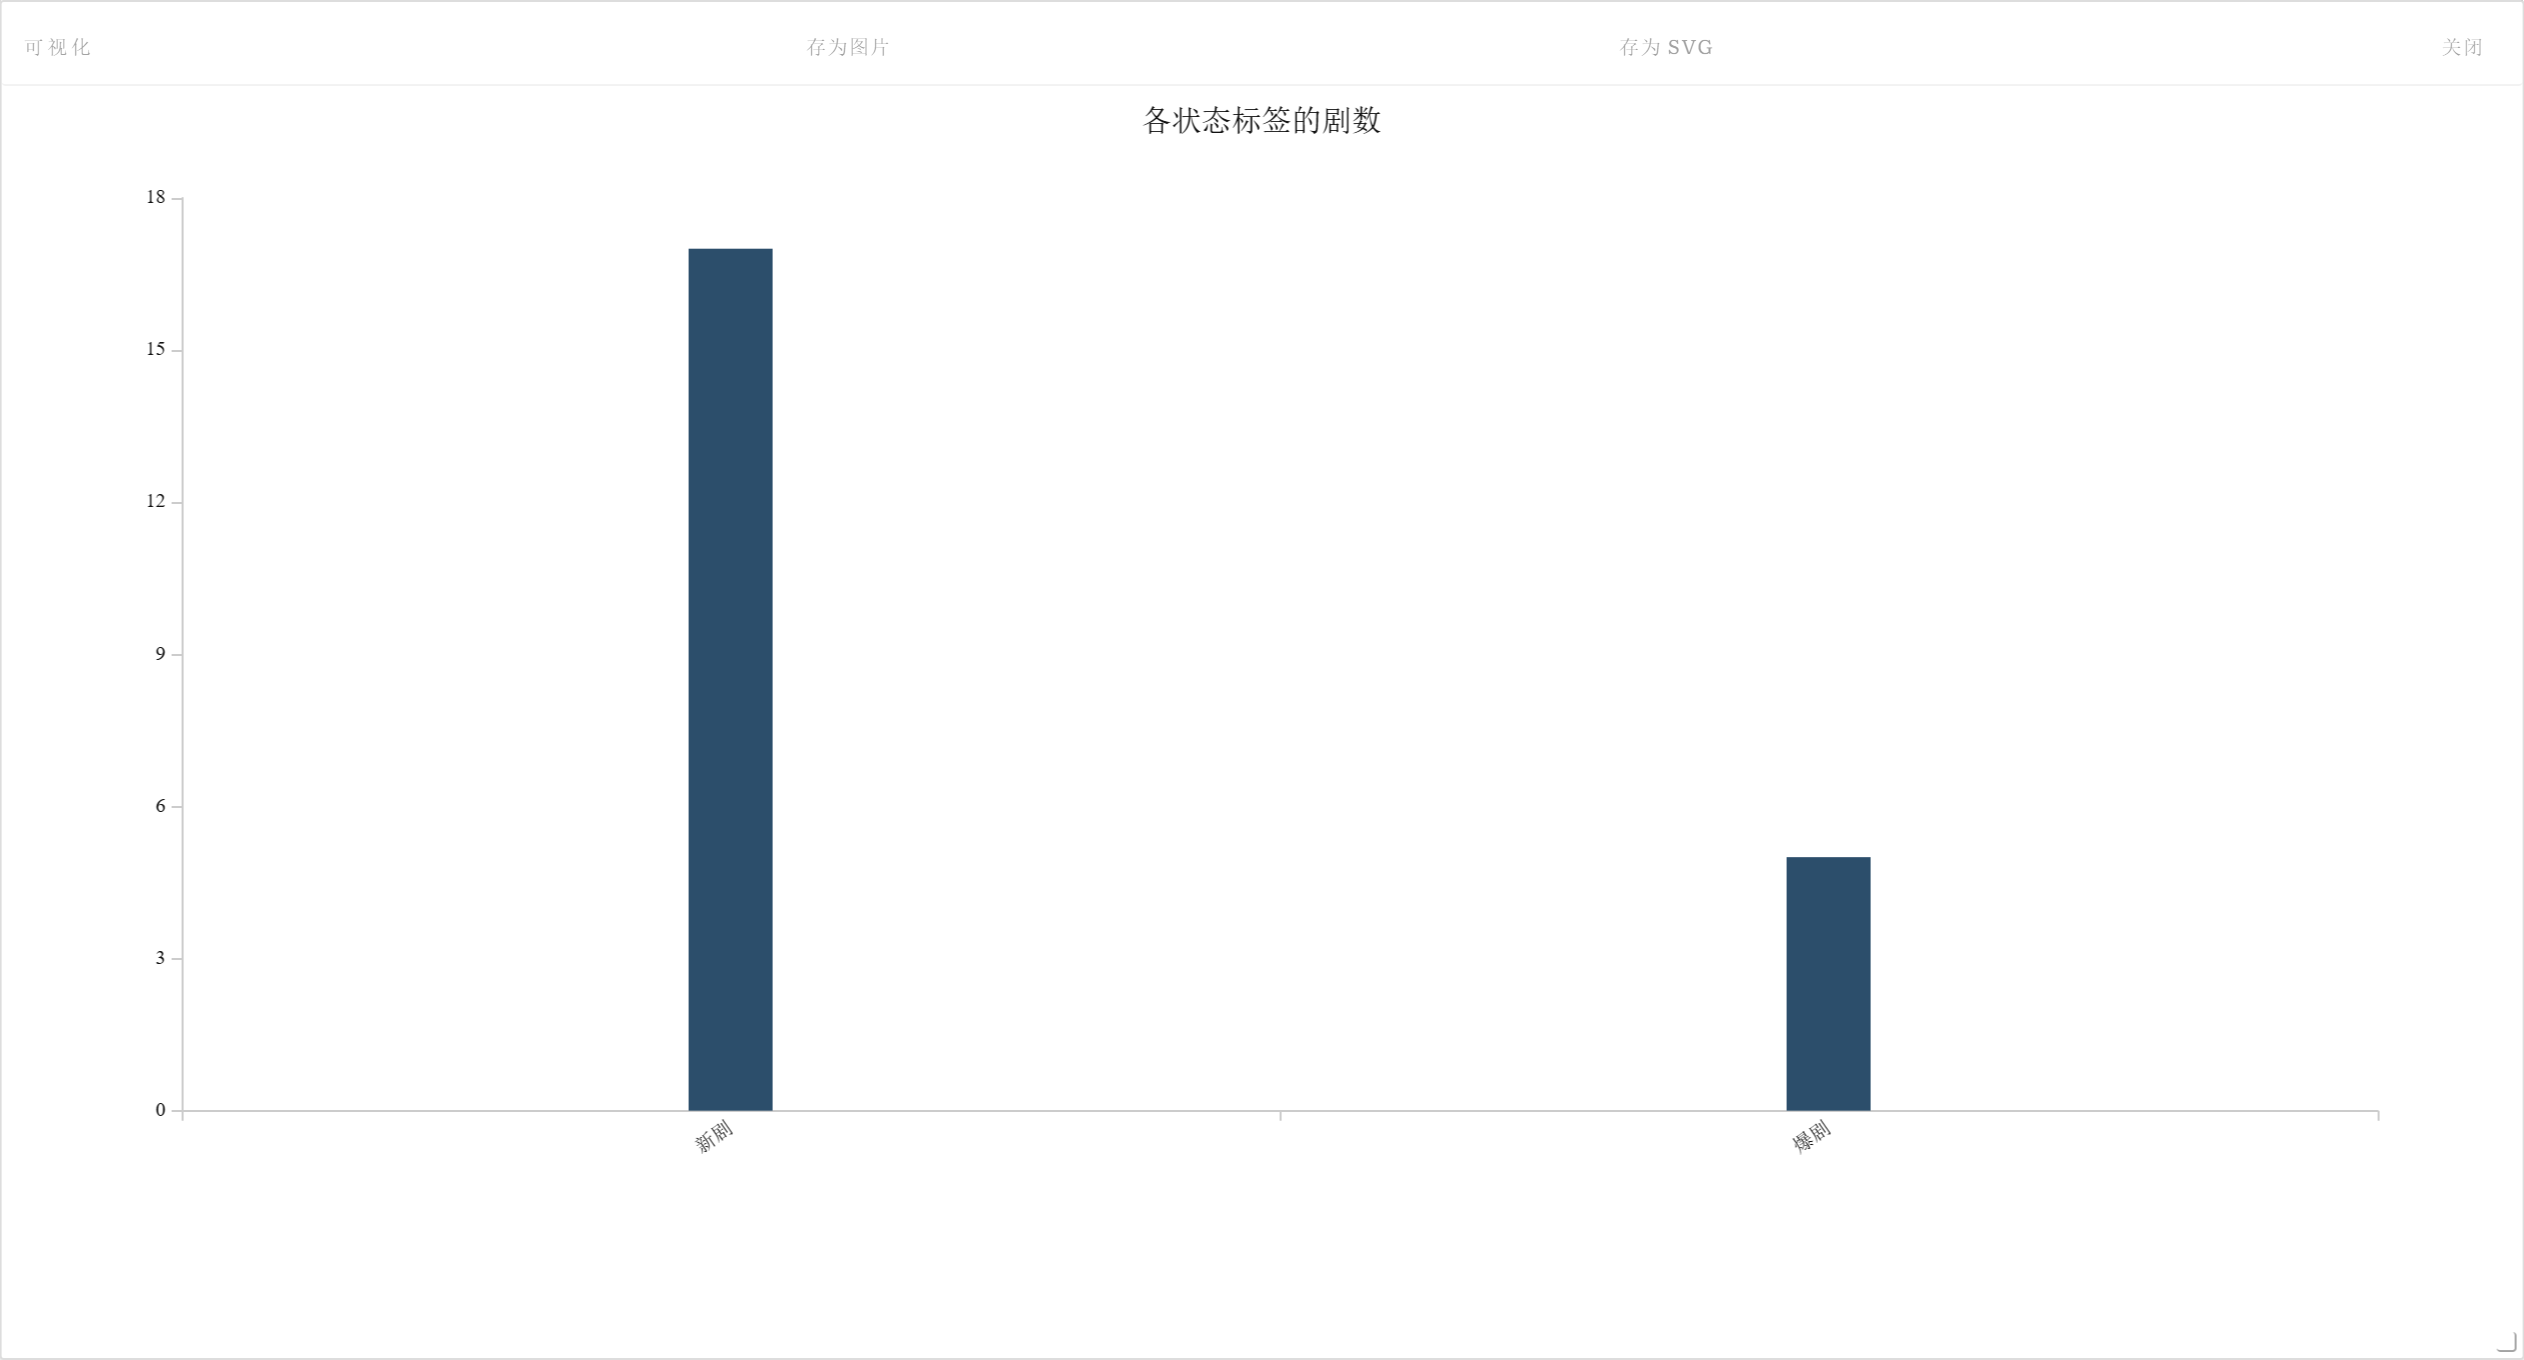
\includegraphics[width=0.96\textwidth]{dashboard-zoom.png}
\caption{从看板点开的全屏图，一个节点一张，可拖动与缩放}
\label{fig:dashboard-zoom}
\end{figure}

菜单条“\texttt{看板}”把画布上所有可视化节点的图拼在一个网格里，一屏看完全部结论。刷新页面会自动回填，
图是数据行的投影，不单独存一份；没有结果的格子写一句先跑一次工作流，是灰字提示，不是报错。

每个格子右上角有“\texttt{全屏}”与“\texttt{存为图片}”，全屏打开的就是上一张图那个浮窗。面板右上角“\texttt{刷新}”重新取数。

\begin{figure}[H]\centering
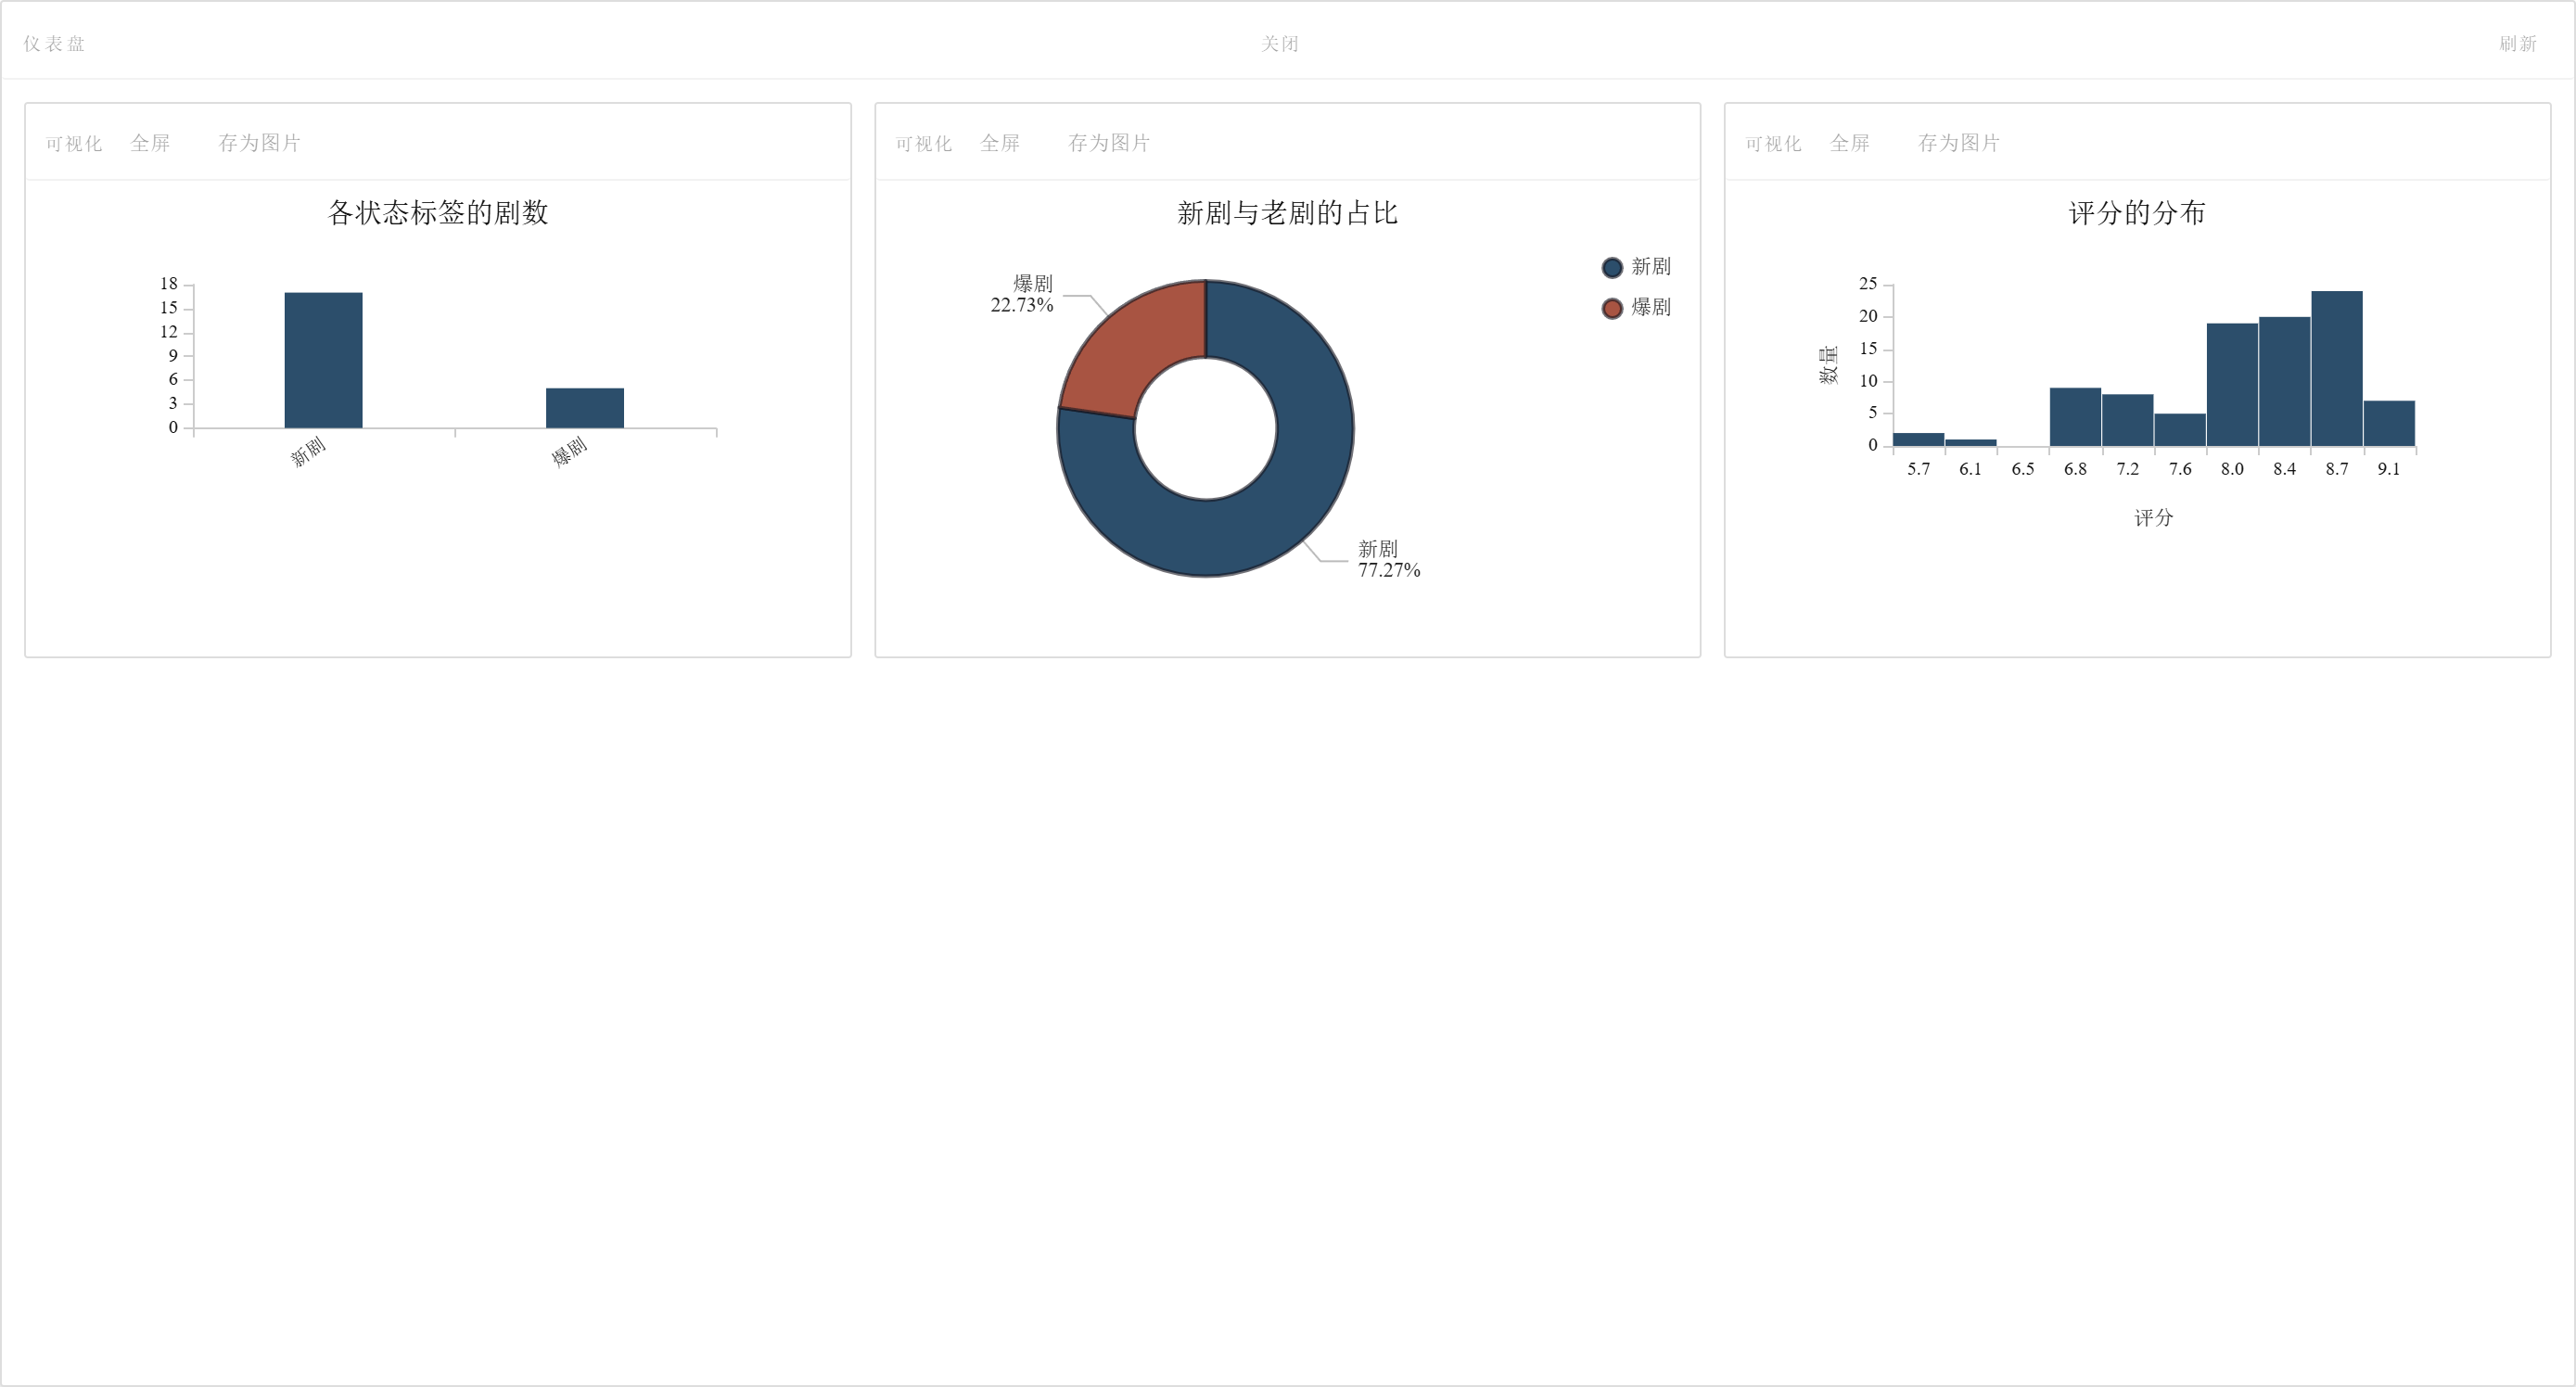
\includegraphics[width=0.98\textwidth]{dashboard.png}
\caption{看板：三个可视化节点并排，每格都能全屏与存图}
\label{fig:dashboard}
\end{figure}

菜单条“\texttt{图表工坊}”是一个内嵌的作图台。可以把任意节点或数据集的整张表交给它自由创作，支持多数据源合并；
自己做好的 PNG 能存回导出目录。适合临时换一种看法，不必为了看一眼而改画布。

\section{报告与执行历史}

工具栏的“\texttt{生成报告}”把一次运行的每张表与服务端渲染的图拼成一个自包含的 HTML，样式与图片都内联，离线能看能打印。
可以附一段模型写的结论，只根据统计数字说话，也可以再打印成 PDF。

“\texttt{历史}”面板按工作流与指标看每次运行的数值走向：情感、倾向、行数三个指标各一条曲线，同一份工作流跑了很多次时，
用它看指标有没有漂移，也能把某次运行的行数与原表对照。

\section{导出与 LaTeX}

\subsection{三种存法}

预览面板和看板每个格子都能把图存成两倍像素的 PNG，或者存成矢量 SVG，文件名就是节点标题，落在导出目录里。
还没有画出来的图不发请求，会提示先预览或者先跑完。数据表则由输出节点存成 CSV、JSON、Excel、文本、HTML、Markdown、Parquet。

\begin{figure}[H]\centering
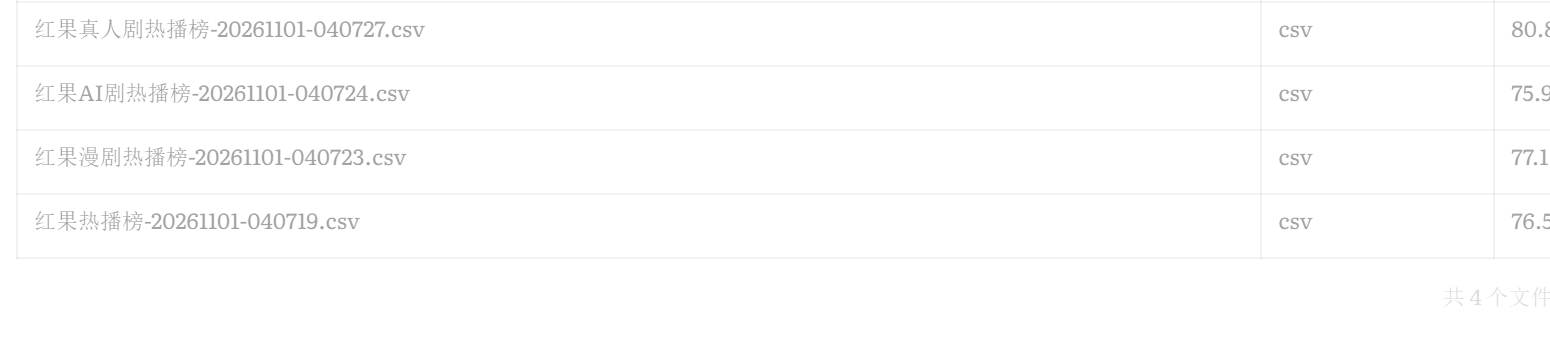
\includegraphics[width=0.96\textwidth]{exports.png}
\caption{导出产物：文件名、类型、大小、修改时间，每行可下载、删除、复制路径}
\label{fig:exports}
\end{figure}

\subsection{LaTeX 图源与三线表}

每个可视化节点默认生成一份 LaTeX 图源，独立文档，xelatex 直接编译成矢量 PDF，也可以把其中的 figure 部分复制进自己的论文。
它对齐手工精修的观感：仿宋、淡网格、千分位、标签带白底圆角框与引线。另有默认开启的三线表，
表格超过一页时会切成整页的块，续块标上续字，一行不丢。

\subsection{编译节点}

编译节点的上游只能是可视化节点，它把图和表合成一份文档，用本机 xelatex 编成一个 PDF。找不到编译器时只让这一个节点失败并说明缺什么，
不会崩掉整轮；编译失败时读的是日志文件而不是屏幕输出，缺宏包与缺字体各有各的说法。输出节点的格式跟着上游走，
接的是可视化或者编译节点时，下拉里只给 PDF。

\subsection{论文成稿}

报告面板里的“\texttt{论文成稿}”只交运行编号与标题。图和表都从这次运行登记过的 LaTeX 源读回来，
所以成稿里的图与预览里的图不可能是两份。前面附方法段，逐节点写出分析单元与参数；后面附工作流名、运行编号、时间窗与图表数。
它先写 tex 再编译，编译器拒绝时留下的就是那份可以继续排查的源文件，不会留半份 PDF。

\section{队列、停止与续跑}

服务同一时刻只跑一轮。再按执行时任务进队列，按钮变成“\texttt{排队运行}”，当前这轮结束自动开始。排队在内存里，重启服务会清空，
所以别把排队当定时任务。队列里有些任务永远起不来：画布走不通、复用的节点坏掉、模型提供方写错，
这类任务入队时就被标上丢弃，轮到时直接跳过并在控制台说明原因，不会一直挡在队首。

停止按钮把正在跑的与还没跑的节点一起停下。已经写下的行保留，节点标成停止，不算失败；有些节点停在一半时把没处理的行留成未处理，
节点算部分完成。这个区别在写方法段时有用。

所有输出与模型答案都落盘，所以一条长链可以分几次做完。

\begin{figure}[H]\centering
\begin{tikzpicture}[node distance=10mm,scale=0.95,transform shape]
  \node[card=src,text width=2.6cm] (run) {运行中};
  \node[card=anl,right=of run,text width=2.8cm] (stop) {中断\\[1pt]\micro 停止、关服务、断电};
  \node[card=viz,right=of stop,text width=2.8cm] (open) {重新打开画布\\[1pt]\micro 顶部横幅};
  \node[card=okc,below=8mm of open,text width=2.8cm] (cont) {继续\\[1pt]\micro 只补缺失部分};
  \node[chip,below=8mm of stop,text width=2.8cm] (fresh) {重新开始\\[1pt]\micro 全量重跑};
  \draw[wire] (run) -- (stop);
  \draw[wire] (stop) -- (open);
  \draw[wire] (open) -- (cont);
  \draw[softwire] (open) -- (fresh);
  \node[micro,right=2mm of cont,text width=3.0cm,align=left] {模型答案走缓存\\ 已付过的钱不再付};
  \node[micro,right=2mm of fresh,text width=3.0cm,align=left] {链短、结果可疑时\\ 用它干净地重来};
\end{tikzpicture}
\caption{中断以后的两条路}
\label{fig:resume}
\end{figure}

重新打开工作流，顶部出现一条检测到中断的运行的横幅。点“\texttt{继续}”，程序只补缺失的部分：已经完成的节点直接复用，
已经处理过的行不再重跑，模型答案从缓存里取。点“\texttt{重新开始}”才算全量重来。

平台那边已经登出、或者数据已经花过钱采过，可以拖一个“\texttt{断点续跑}”节点，直接把历史运行的输出行收过来当输入，从那里接着往下做。
它不重新爬，只读取已经存下的行。

节点完成以后，只要上游没变，再次运行到它就复用上次的结果，新加几个节点也不影响旧的。要让某个节点重算，用“\texttt{从此节点重跑}”，
它和下游重算，上游照旧拿。

\section{运行台账}

运行记录里有一行一次的运行编号、工作流名、状态、模式、开始与结束时间、节点数、行数。每个节点每次运行的表格输出按运行号存着，
随时能翻出来看真实的行，也能导出。日志按运行号持久化，按级别与工作流过滤，能下载成文本。右侧的动作能载入这次结果到画布、
打开日志、生成报告、删除这条记录。

\begin{figure}[H]\centering
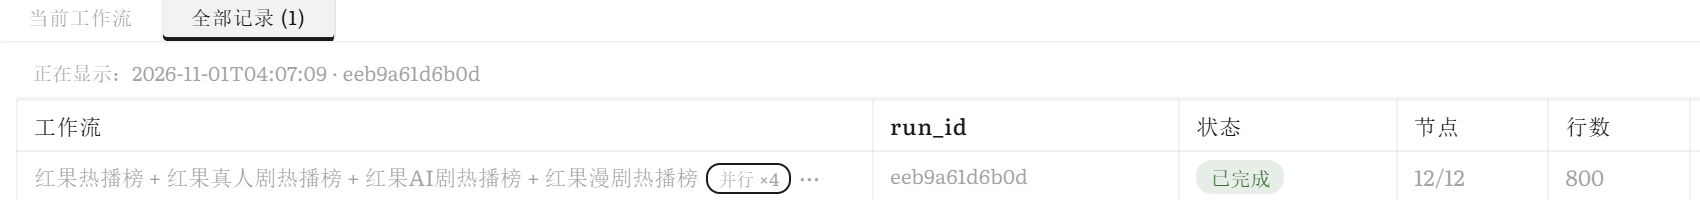
\includegraphics[width=0.96\textwidth]{runs.png}
\caption{运行记录的一行：状态、节点数、行数、耗时与操作}
\label{fig:runs}
\end{figure}

导出产物面板集中显示所有落盘文件，按运行清理，也可以一次清空，下载、删除、复制路径都在每一行上。
运行库会随时间变大，运行记录可以按条删除，导出产物可以按运行清理，删一条运行不动别的运行的行。

数据目录不在版本库里，只有工作流文件例外，所以除了远端仓库还需要一个还原点。备份工具生成一份代码包与一份数据归档，
覆盖系统数据与每个账号自己的库与工作流，默认不含 Cookie。

“\texttt{工作流文件}”面板能导出项目包，包里是工作流、被引用的数据集与可复用模板，换一台机器导入以后接着用，不用重新挂数据。
单独导入一份工作流文件就只是加一份画布。

\begin{figure}[H]\centering
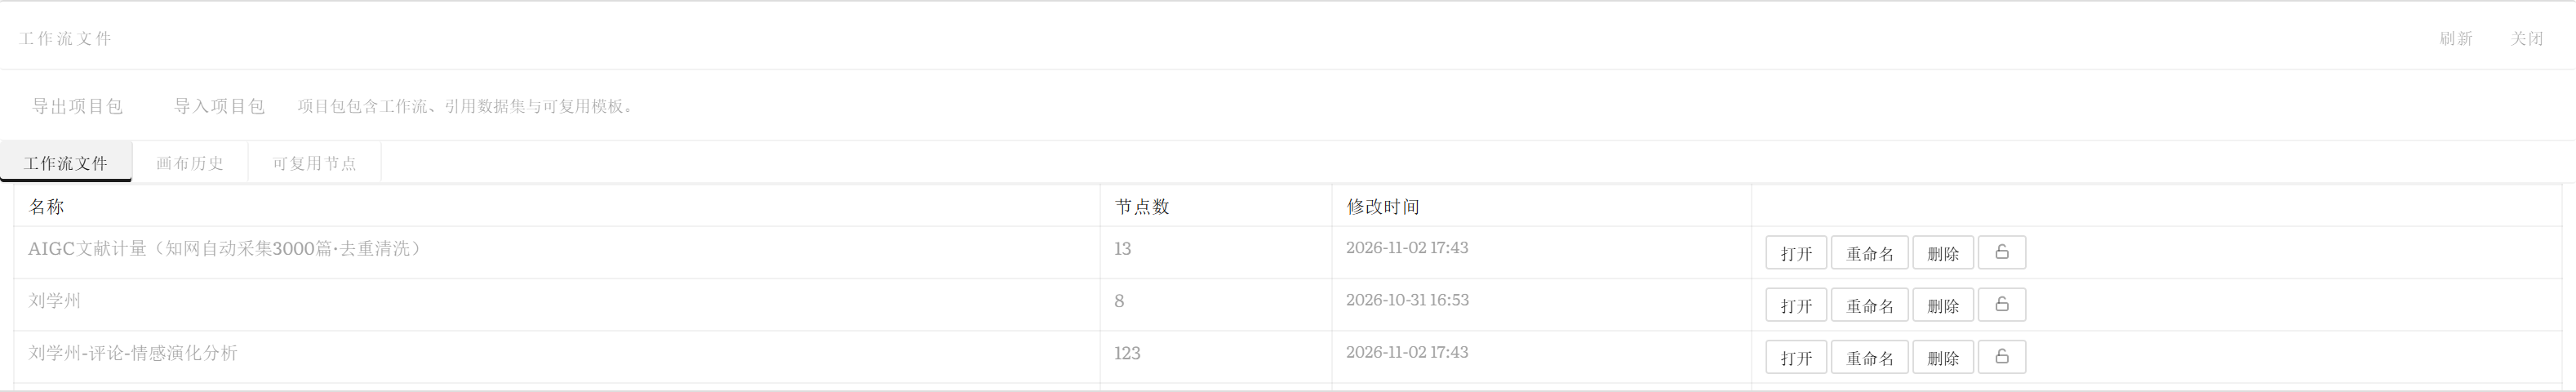
\includegraphics[width=0.92\textwidth]{workflows.png}
\caption{工作流文件：打开、重命名、导入导出、打包成项目}
\label{fig:workflows}
\end{figure}

\section{定时任务}

定时任务由应用内的一只时钟驱动，跟着服务一起启动。到点执行一张已存画布，可以按天、按周、按间隔，也可以写五段 cron；
每个任务可以指定自己的时区，留空按服务器本地时间。面板显示服务器时间、时钟是否在跑、每个任务的下次运行与最近一次结果。

\begin{figure}[H]\centering

\includegraphics[width=0.98\textwidth]{schedules.png}
\caption{定时任务：触发句子、下次运行、启用与立即执行}
\label{fig:schedules}
\end{figure}

含模型节点的画布不能定时。选择画布时就标明不能定时并写出原因，不会等到半夜才失败，因为半夜没人看着花 token 不是好事。

服务停机期间错过的点只记一条已错过，不会在开机时补跑一批。到点的任务与手动执行走同一条启动路径，服务忙就排队；
启动失败写进这个任务自己的历史，不写进运行控制台。下次时间、上次结果、任务句子与能不能跑，全由服务端算好送来，面板不自己猜。

\section{账号与云端}

一个人本机用不需要账号。放到服务器上给多人用就要开云端模式：它会关掉本地模型界面、强制无头抓取、拒绝浏览器生成登录，
并且强制账号登录。已经部署好的那份在 \texttt{http://47.116.114.77/crawler}，打开就能看见登录页；自己开一份也可以，
只要在启动前设好管理员密码与会话密钥，否则按名字拒绝启动。密码用 scrypt 哈希，会话在服务端，带 CSRF 与失败锁定。

\begin{figure}[H]\centering
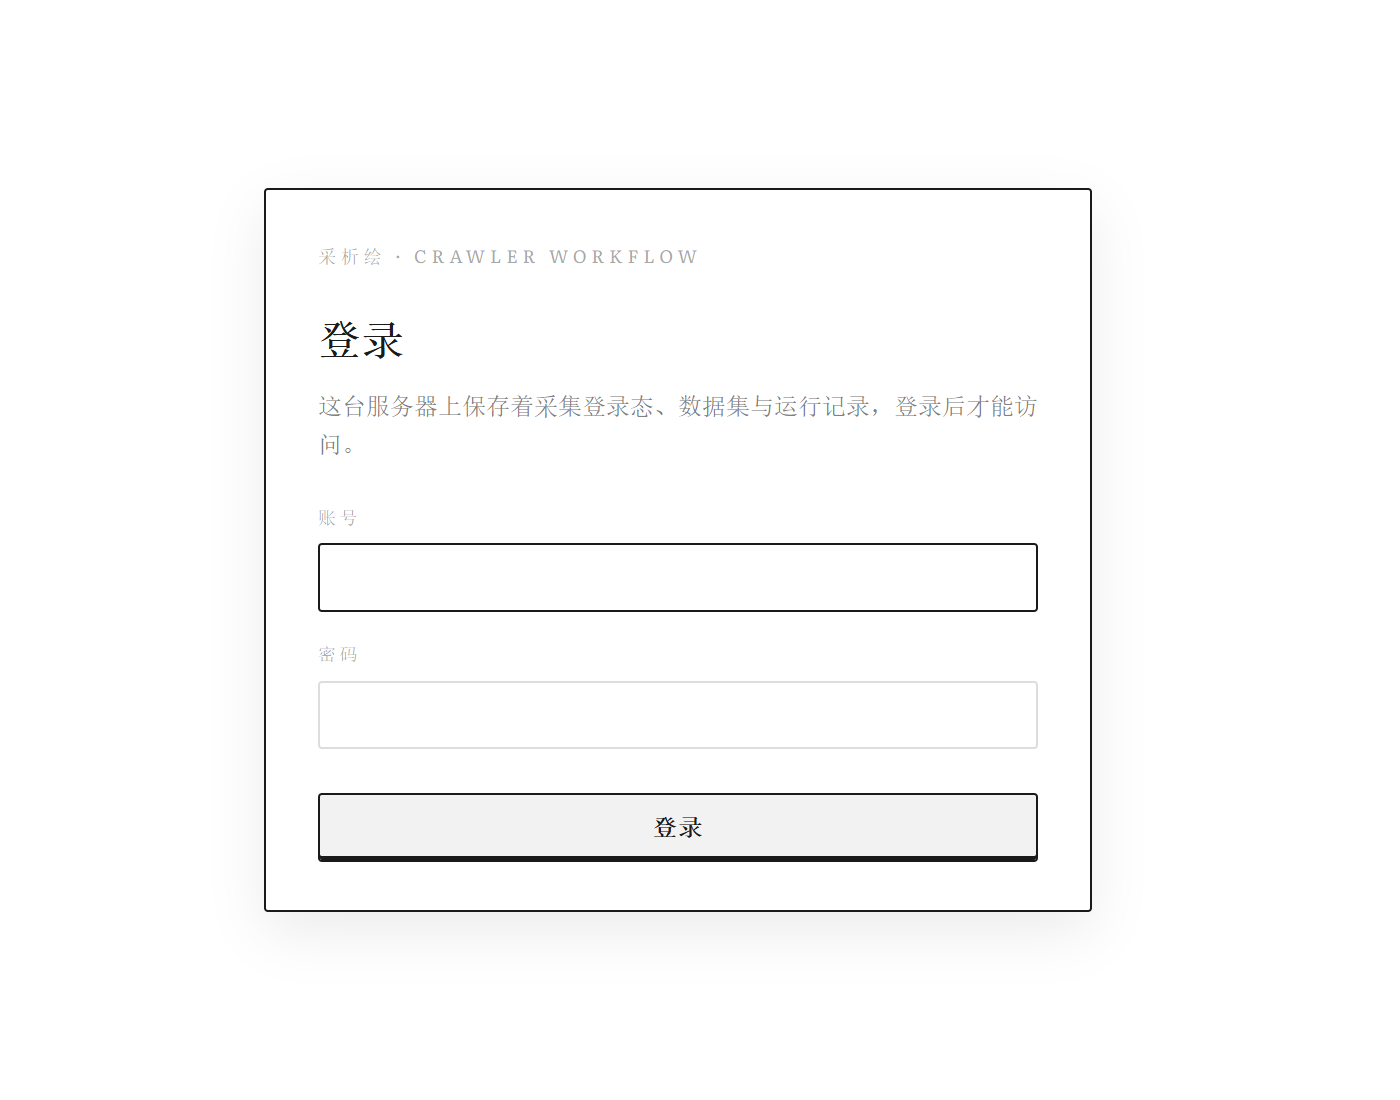
\includegraphics[width=0.5\textwidth]{login.png}
\caption{云端登录页：一条地址，两个输入框}
\label{fig:login}
\end{figure}

密码错一次就是一句话，不会告诉你账号存不存在，也不会告诉你是不是被锁了。连续错到上限会被锁一段时间，这段时间换一个浏览器也没用。
管理员刚开出来的账号带一个临时密码，第一次登录会要求改掉，这一屏不能关；改完以后顶栏右侧出现账号名与退出登录，画布才恢复正常。

\begin{figure}[H]\centering
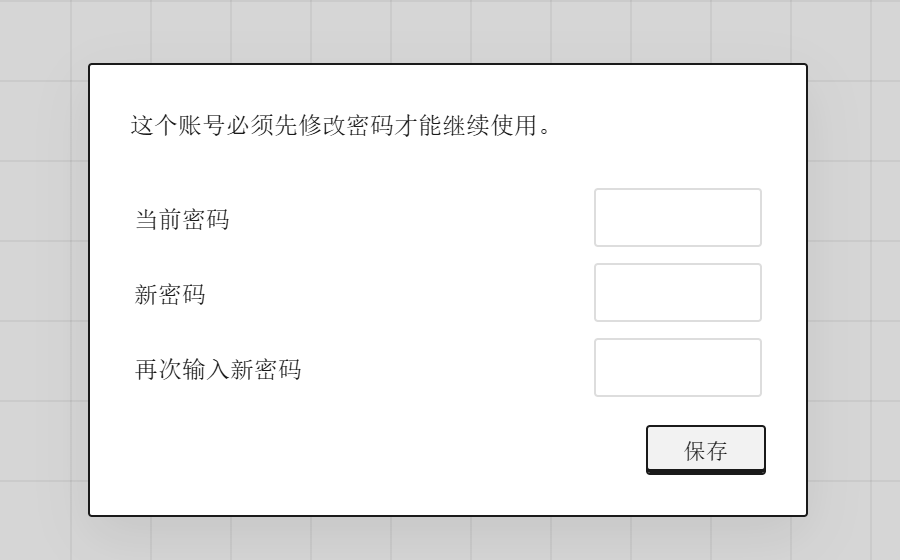
\includegraphics[width=0.44\textwidth]{force-password.png}
\caption{首次登录的强制改密：当前、新、确认}
\label{fig:force-password}
\end{figure}

管理员点顶栏的账号名打开账号管理：上面三个输入框建号，下面一行一个人，能重置密码、强制下线，普通用户还能禁用与删除。
状态列写启用、待改密、已禁用；最近操作是审计，谁在什么时候登录、改密、建号、删号，一条条记着，时间按你所在时区显示。
删除是把这个人整棵数据目录移进回收站，不会当场抹掉；强制下线只踢掉当前会话。

\begin{figure}[H]\centering
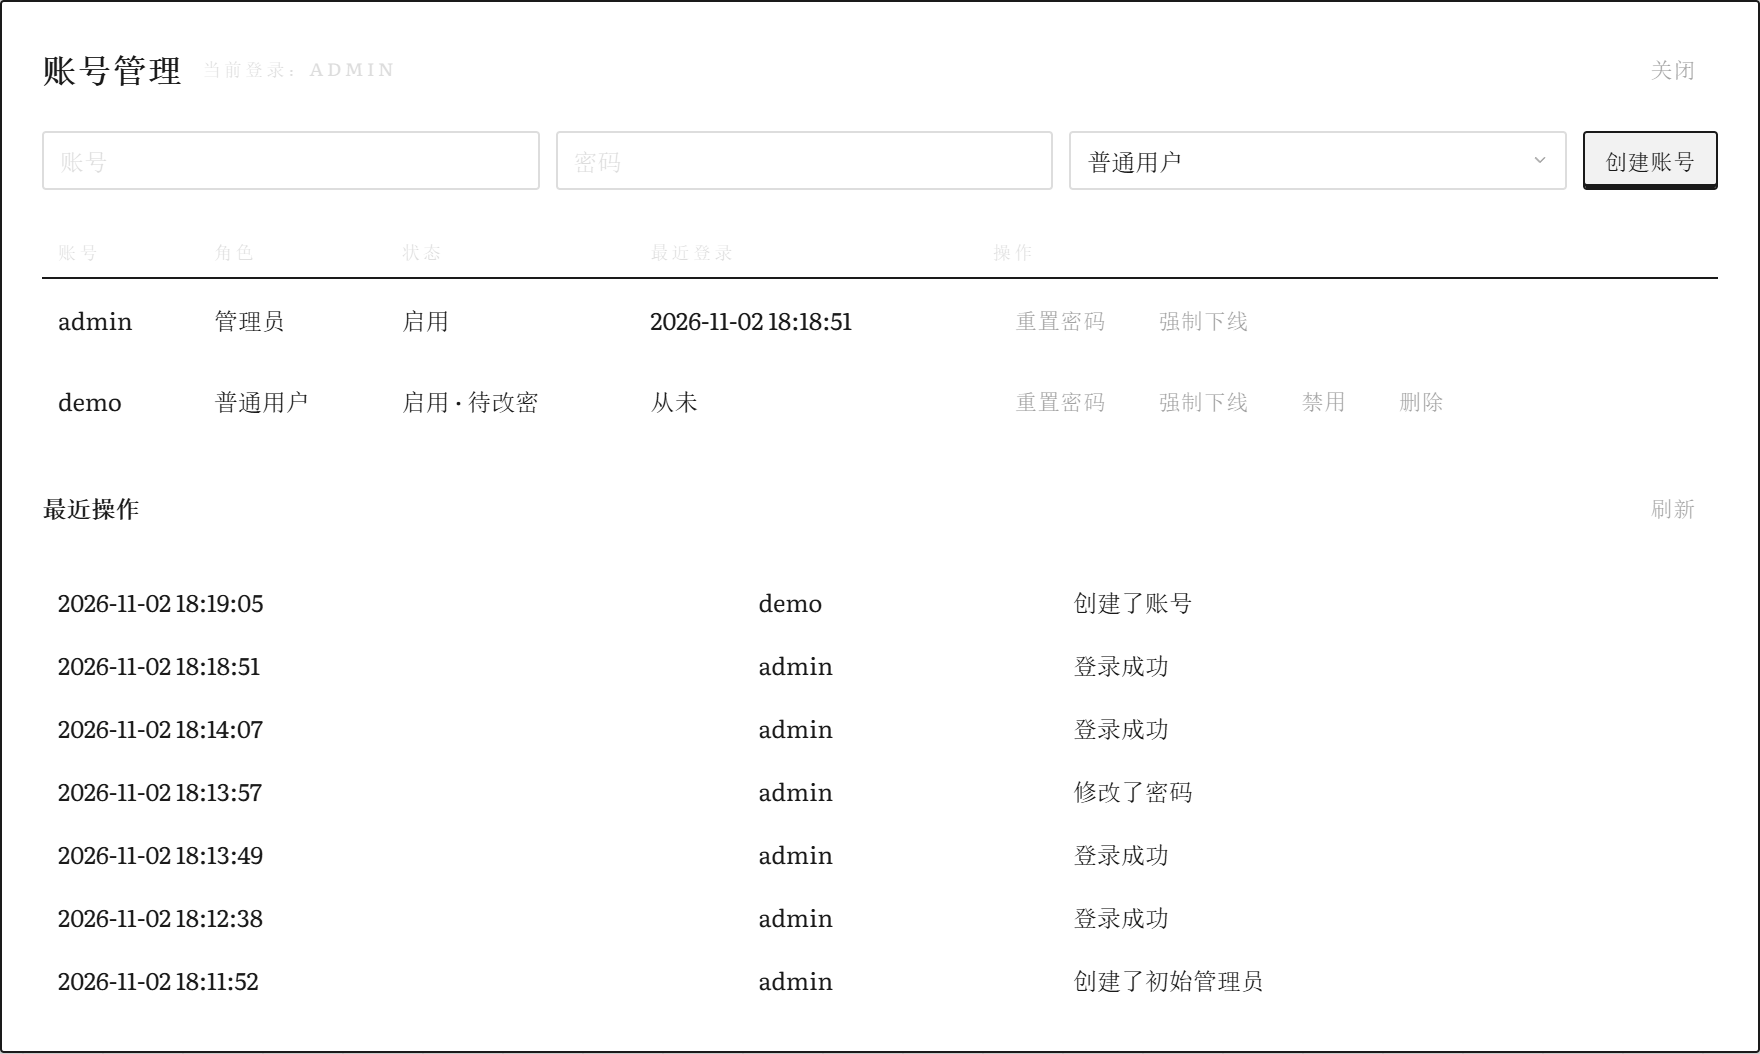
\includegraphics[width=0.94\textwidth]{accounts.png}
\caption{账号管理：角色、状态、最近登录与操作}
\label{fig:accounts}
\end{figure}

每个账号一棵目录树，工作流、数据集、运行记录、登录状态、导出全在里面，运行也互不可见：状态、停止、进程、统计只答自己那一次。
旧版单账号的数据根可以迁到管理员名下，工具默认只演练，确认以后才动手，迁移前先备份，原目录改名保留。

没开账号时把监听地址改成非本机，等于把已保存的登录状态与数据集开放给整个局域网，程序会拒绝启动。这不是多余的限制。

\section{外观、词库与设置}

中英两套文案，切换即时生效，只影响显示，不改数据。主题有自动、浅色、深色三档，自动跟随系统，图表配色一起换。
圆角有一个统一滑杆，改完全界面一起变。

\begin{figure}[H]\centering
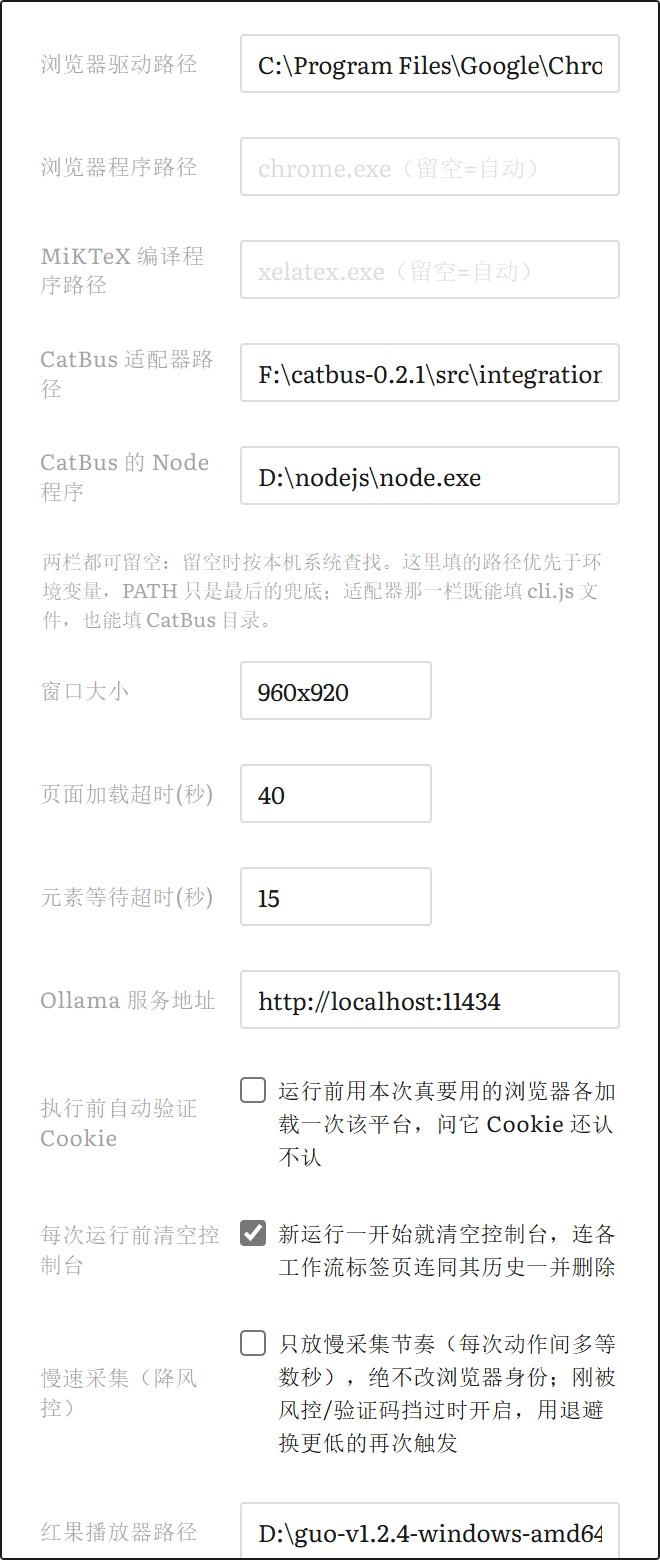
\includegraphics[width=0.5\textwidth]{settings-menu.png}
\caption{设置菜单：驱动路径、浏览器、超时、Cookie 预检、编译程序都在这里}
\label{fig:settings}
\end{figure}

设置面板里能改 Chrome 驱动与浏览器路径、窗口尺寸、页面与元素超时、慢速采集、Cookie 预检开关、同平台排队与错峰，
也能指定编译程序路径与模型服务地址。这些写进配置文件，下次运行直接生效，不用改代码重启。

“\texttt{词库}”面板管停用词与领域词。停用词在关键词、主题、词云与机器学习里都会过滤，领域词写进分词词典，
改动从下一次运行开始生效。

\begin{figure}[H]\centering
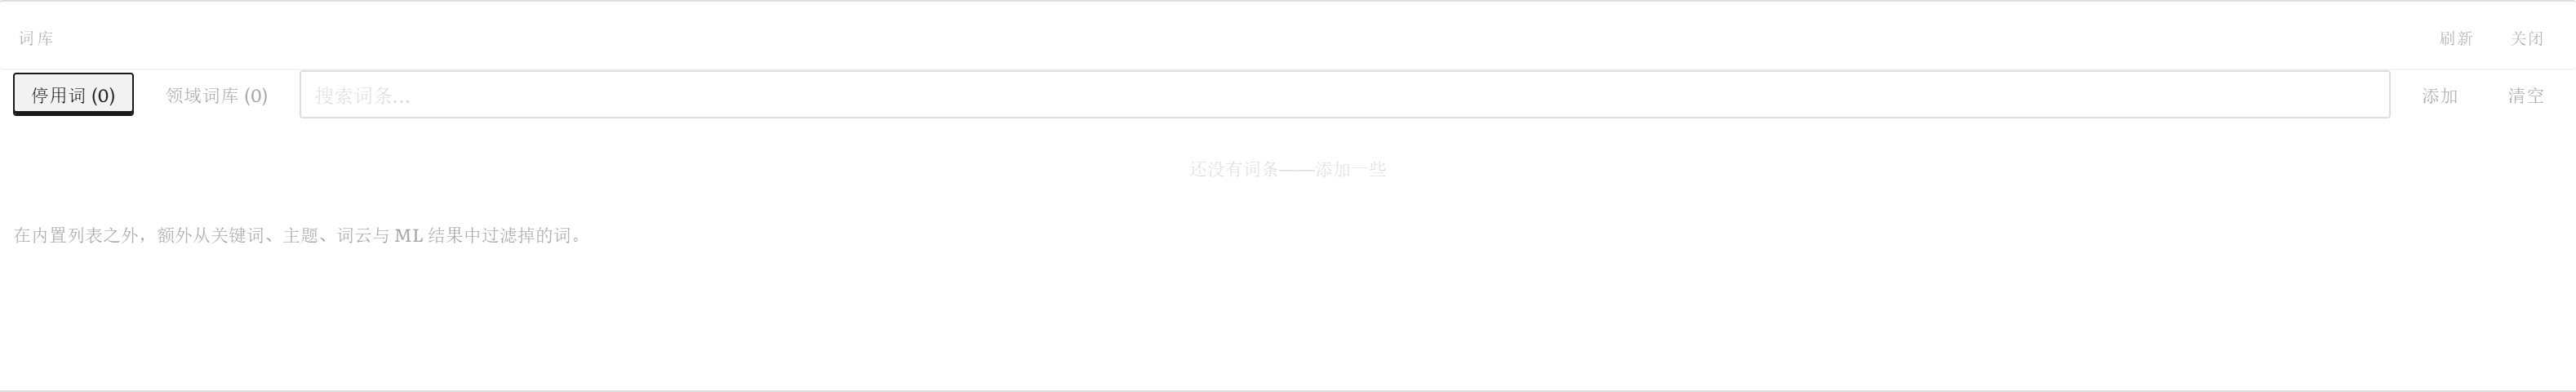
\includegraphics[width=0.43\textwidth]{lexicon.png}
\caption{词库：停用词与领域词}
\label{fig:lexicon}
\end{figure}

深色主题是同一套令牌的另一组取值，图表、节点、面板一起换，导出的 PNG 也跟着换。晚上看画布舒服一些，打印前记得换回浅色。

\begin{figure}[H]\centering
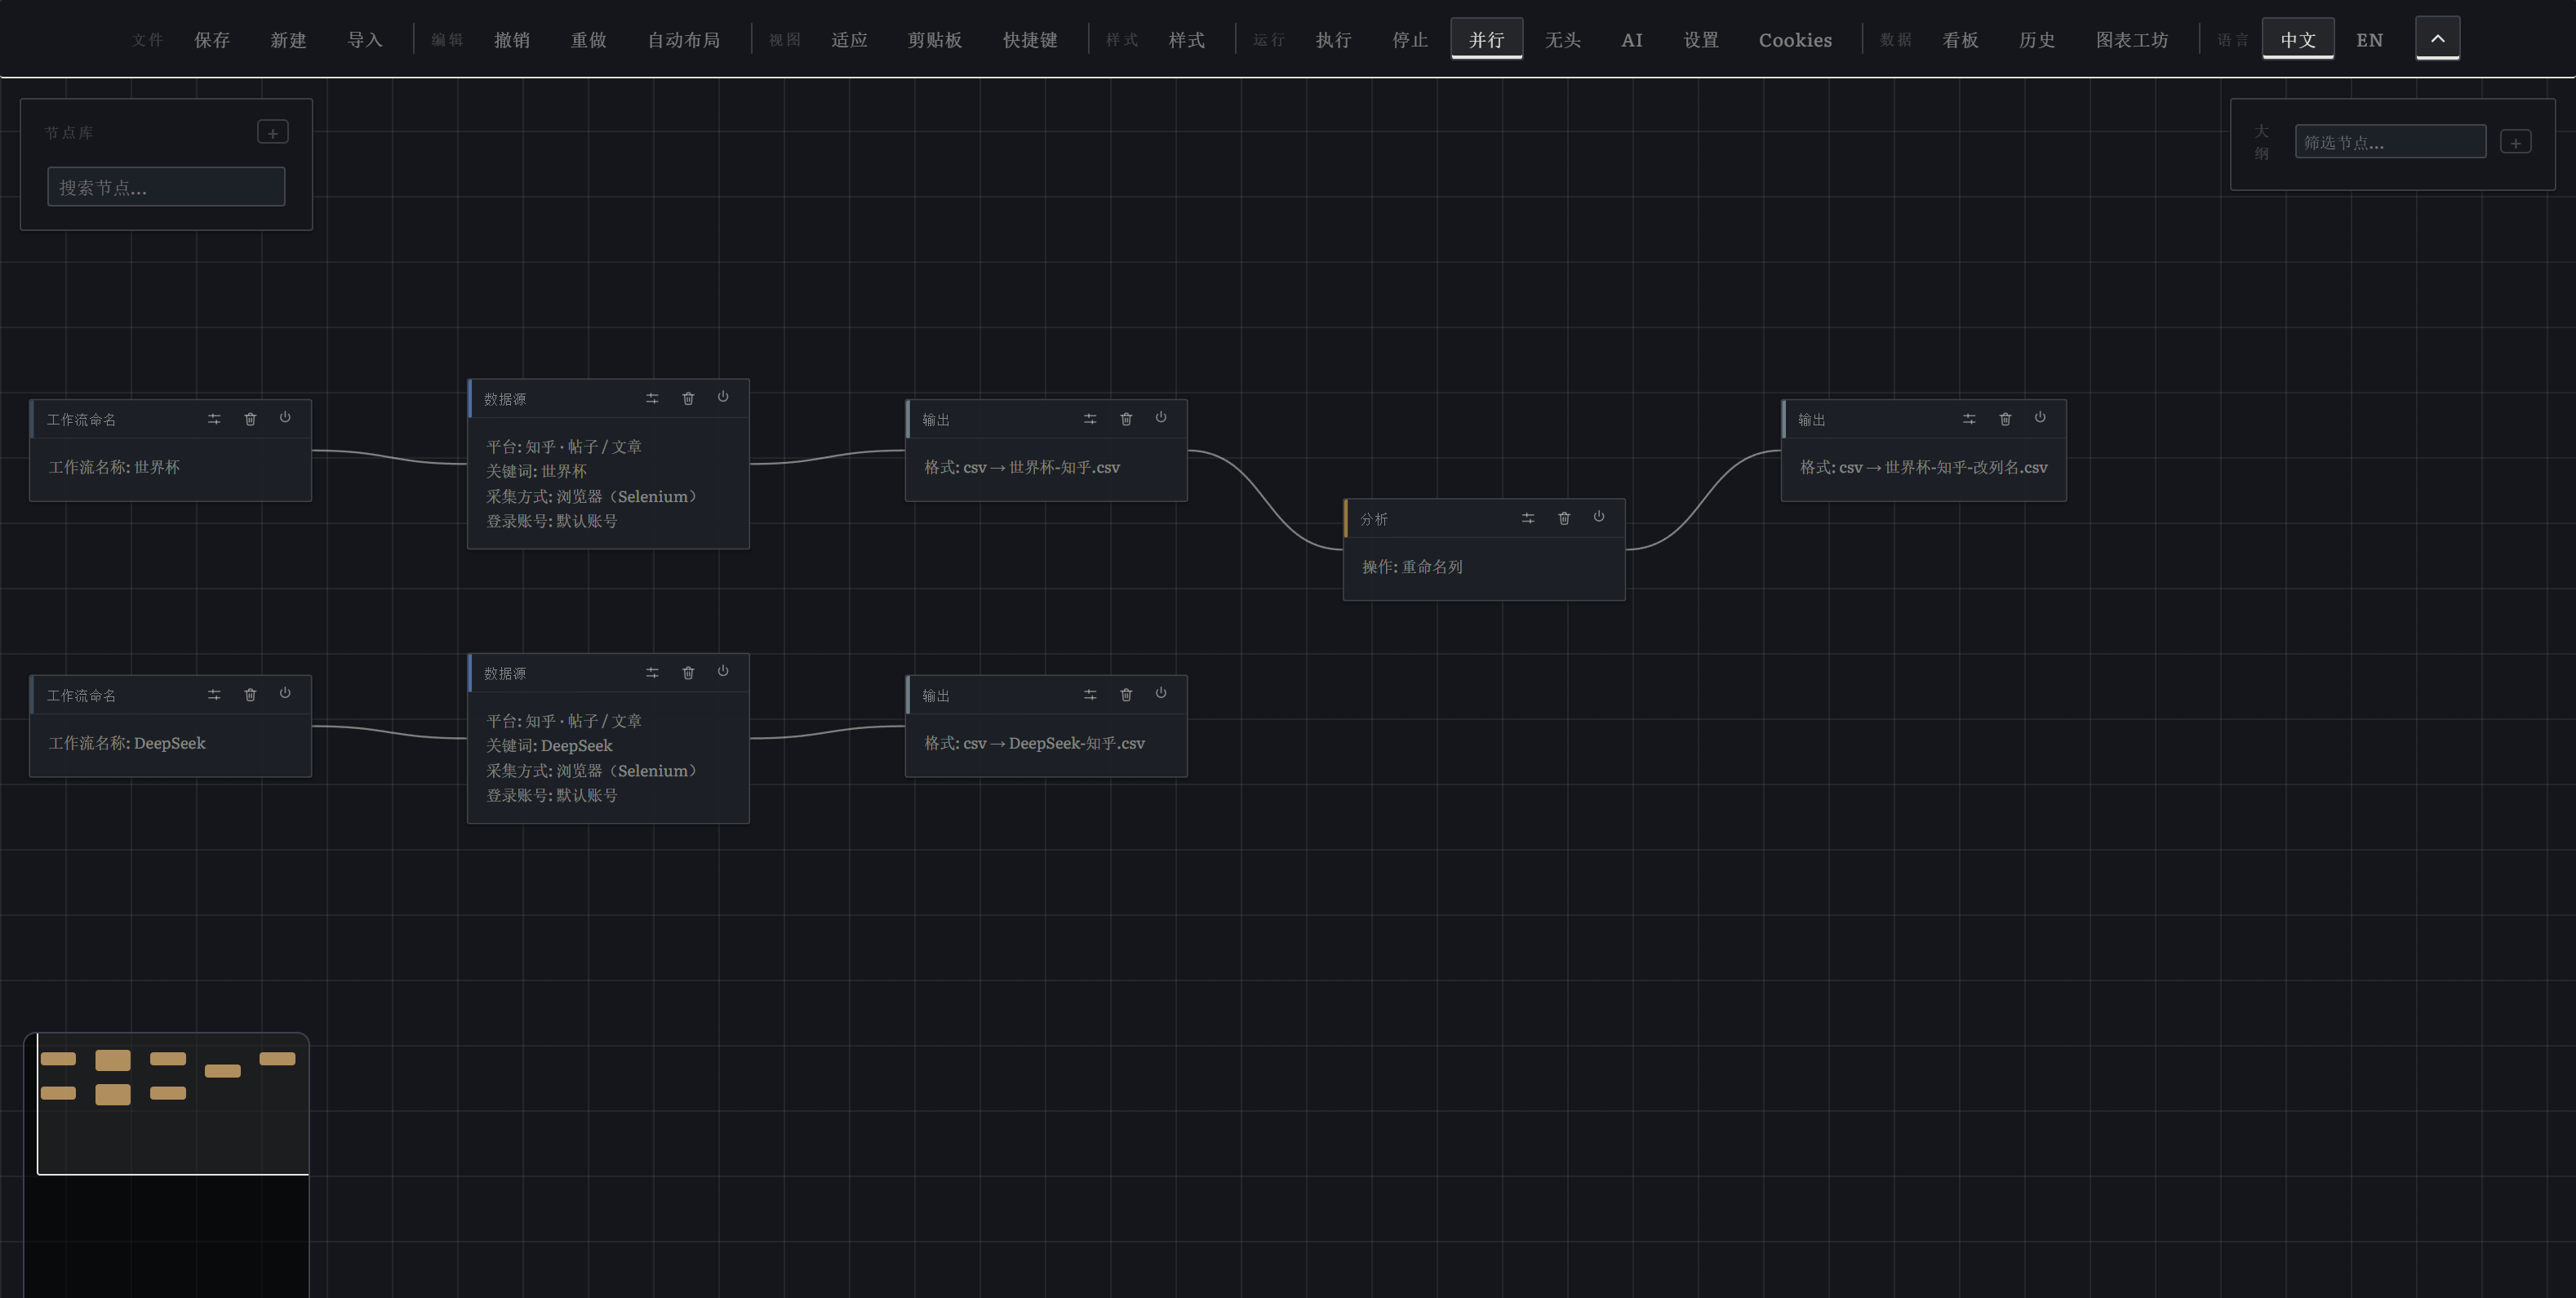
\includegraphics[width=0.96\textwidth]{dark.png}
\caption{深色主题下的画布}
\label{fig:dark}
\end{figure}

\section{打包给别人}

不装 Python 的人用桌面版。它把后端与前端打成一个目录，双击启动本地服务并打开浏览器；数据默认放在用户目录，
exe 旁边放一个空文件就切便携模式，安装包是可选的。微调模型不放应用包里，单独发一个模型包，解压到同级目录自动登记；
不放也能用，相关节点降级并在控制台写明实际用了哪种模式。打包只针对 Windows，Linux 与 macOS 用源码跑，装好 Chrome 与中文字体即可。

\section{被拒绝的时候看哪里}

这个软件遇到不确定的事一律按名字拒绝，不猜。拒绝的话里通常写了原因与下一步。先看控制台那一行，再看节点设置面板顶部的校验提示。

\begin{table}[H]\centering
\caption{常见拒绝与处理}
\label{tab:refuse}
\small
\begin{tabularx}{\textwidth}{p{4.4cm}X}
\toprule
看到的话 & 通常怎么做 \\
\midrule
找不到驱动，或版本不符 & 在设置里填本机 chromedriver 的路径，版本要和 Chrome 一致 \\
登录墙，或账号没有登录状态 & 在 Cookies 面板重新存一份，或换一个已保存的账号 \\
缺模型，或模型跑不动 & 确认 Ollama 在跑、模型名对得上，或换一种分析模式 \\
缺列，或列名不对 & 打开上游节点的设置，看它实际输出哪些列 \\
该组合不可用 & 这个平台没有这个功能，换采集内容或换后端 \\
缺 ctex，或缺 FangSong & TeX 发行版补中文支持，Windows 上装完整版 MiKTeX \\
服务已在运行 & 先停掉旧实例，或给新实例一份自己的数据目录 \\
数据集不在库里 & 换机器时把整个 data 目录一起搬过来 \\
\bottomrule
\end{tabularx}
\end{table}

最后两件小事。数据目录不要随手删，工作流只记数据集编号，换个目录就打不开了；Chrome 驱动不要让工具自己去下载，
本机装好一份、指过去，跑起来最稳。


\end{document}
